%% 
%% Copyright 2019-2020 Elsevier Ltd
%% 
%% This file is part of the 'CAS Bundle'.
%% --------------------------------------
%% 
%% It may be distributed under the conditions of the LaTeX Project Public
%% License, either version 1.2 of this license or (at your option) any
%% later version.  The latest version of this license is in
%%    http://www.latex-project.org/lppl.txt
%% and version 1.2 or later is part of all distributions of LaTeX
%% version 1999/12/01 or later.
%% 
%% The list of all files belonging to the 'CAS Bundle' is
%% given in the file `manifest.txt'.
%% 
%% Template article for cas-sc documentclass for 
%% single column output.

%\documentclass[a4paper,fleqn,longmktitle]{cas-sc}
\documentclass[a4paper,fleqn]{cas-sc}

%\usepackage[numbers]{natbib}
%\usepackage[authoryear]{natbib}
\usepackage[authoryear,longnamesfirst]{natbib}


\usepackage[figuresright]{rotating}

%########################################################################################
%            						PACKAGES
%########################################################################################

\usepackage{pdfpages}
%\usepackage{authblk} % for author affiliations
\usepackage{amsmath,amssymb,bbm,mathrsfs,mathtools,xfrac} %math stuff
\usepackage{amsthm}
%\newtheorem{theorem}{Theorem}
%\newtheorem{lemma}{Lemma}

%\usepackage{cleveref}
%\newcommand{\crefrangeconjunction}{--}
%\usepackage[nomarkers,figuresonly]{endfloat}

%\usepackage[sort]{natbib}   % bibliography omit 'round' option if you prefer square brackets
\usepackage{placeins} % for \FloatBarrier
\usepackage[utf8]{inputenc} % for french accents
\usepackage[T1]{fontenc} % for french accents
\usepackage{ctable} % load after tikz. used for tables
\usepackage{pifont}% http://ctan.org/pkg/pifont
\newcommand{\cmark}{\ding{51}}%
\newcommand{\xmark}{\ding{55}}%
\def\widebar#1{\overline{#1}}
\usepackage{array}
%\newcolumntype{L}{>{\centering\arraybackslash}m{3cm}} % used for text wrapping in ctable
\usepackage{color, colortbl, xcolor, comment}
\usepackage{subfig}
%\usepackage{tcolorbox} % for box around text
%\usepackage[ruled,vlined,linesnumbered,noresetcount]{algorithm2e}
%\usepackage[ruled,vlined,noresetcount]{algorithm2e}
\usepackage{algorithm}
\usepackage{chngcntr} % for figure labels in appendix
%\usepackage[ruled,vlined,noresetcount]{algorithm2e}
\usepackage[noend]{algpseudocode}
\algrenewcommand\textproc{}% Used to be \textsc
\algdef{SE}[SUBALG]{Indent}{EndIndent}{}{\algorithmicend\ }%
\algtext*{Indent}
\algtext*{EndIndent}
%\usepackage[american]{babel}
%\let\tnote\relax

%\usepackage{csquotes}

\usepackage{pdflscape}

%\usepackage[style=apa,sortcites=true,sorting=nyt,backend=biber]{biblatex}
%\usepackage{epstopdf}

%\usepackage{tabulary}
%\usepackage{siunitx}
%\sisetup{output-exponent-marker=\ensuremath{\mathrm{e}}}
%\AtBeginEnvironment{tabulary}{\onehalfspacing}
%\usepackage{multirow}
%\usepackage{ctable} % NEED TO LOAD CTABLE AFTER TIKZ FOR SOME REASON
%\usepackage{array}
%\newcolumntype{L}{>{\centering\arraybackslash}m{3cm}} % used for text wrapping in ctable
%\usepackage{enumitem}
% These packages are all incorporated in the memoir class to one degree or another...


%%%Author macros
\def\tsc#1{\csdef{#1}{\textsc{\lowercase{#1}}\xspace}}
\tsc{WGM}
\tsc{QE}
\tsc{EP}
\tsc{PMS}
\tsc{BEC}
\tsc{DE}
%########################################################################################
%            						CUSTOM COMMANDS
%########################################################################################

\newtheorem{theorem}{Theorem}
\newtheorem{proposition}{Proposition}
\newtheorem{lemma}{Lemma}
\newcommand{\sgn}{\operatorname{sgn}}
\newcommand{\Op}{O_{P}}
\newcommand{\op}{o_{P}}
\newcommand{\ddd}{,\ldots,}
%\global\long\def\ddd{,\ldots,}
\newcommand{\sail}{\texttt{sail}}
\newcommand{\tm}[1]{\textrm{{#1}}}
\newcommand{\bx}{\textbf{\emph{x}}}
\newcommand{\by}{\textbf{\emph{y}}}
\newcommand{\bX}{\textbf{\emph{X}}}
\newcommand{\bW}{\textbf{\emph{W}}}
\newcommand{\bY}{\textbf{\emph{Y}}}
\newcommand{\bD}{\textbf{\text{D}}}
\newcommand{\bXtilde}{\widetilde{\bX}}
\newcommand{\bYtilde}{\widetilde{\bY}}
\newcommand{\bDtilde}{\widetilde{\bD}}
\newcommand{\Xtilde}{\widetilde{X}}
\newcommand{\Ytilde}{\widetilde{Y}}
\newcommand{\Dtilde}{\widetilde{D}}
\newcommand{\bu}{\textbf{u}}
\newcommand{\bU}{\textbf{\emph{U}}}
\newcommand{\bV}{\textbf{\emph{V}}}
\newcommand{\bE}{\textbf{\emph{E}}}
\newcommand{\bb}{\textbf{\emph{b}}}
\newcommand{\bI}{\textbf{\emph{I}}}
\newcommand{\be}{\boldsymbol{\varepsilon}}
\newcommand{\bSigma}{\boldsymbol{\Sigma}}
\newcommand{\bLambda}{\boldsymbol{\Lambda}}
\newcommand{\bTheta}{\boldsymbol{\Theta}}
\newcommand{\balpha}{\boldsymbol{\alpha}}
\newcommand{\btau}{\boldsymbol{\tau}}
\newcommand{\bgamma}{\boldsymbol{\gamma}}
%\newcommand{\ltwonorm}[1]{\lVert #1 \rVert}
\newcommand{\mb}[1]{\mathbf{#1}}
\newcommand{\mc}[2]{\multicolumn{#1}{c}{#2}}
\newcommand{\mcl}[2]{\multicolumn{#1}{l}{#2}}
\definecolor{Gray}{gray}{0.9}
\newcommand {\bs}{\boldsymbol}
%\newcommand{\norm}[1]{\left\Vert #1 \right\Vert}
\newcommand{\xf}{\mathcal{X}}
\newcommand{\pfrac}[2]{\left( \frac{#1}{#2}\right)}
\newcommand{\e}{{\mathsf E}}
\newcommand{\bt}{\boldsymbol{\theta}}
\newcommand{\bmu}{\boldsymbol{\mu}}
\newcommand{\bbeta}{\boldsymbol{\beta}}
\newcommand{\btheta}{\boldsymbol{\theta}}
\newcommand{\bPhi}{\boldsymbol{\Phi}}
\newcommand{\bPsi}{\boldsymbol{\Psi}}
\DeclareMathOperator*{\argmin}{arg\,min}
\DeclareMathOperator*{\argmax}{arg\,max}
\DeclareMathOperator{\diag}{diag} % operator and subscript

\DeclarePairedDelimiter\abs{\lvert}{\rvert}%
\DeclarePairedDelimiter\norm{\lVert}{\rVert}%

\global\long\def\ddd{,\ldots,}


\newcommand{\bthetastar}{\boldsymbol{\theta}^{*}}
\newcommand{\bThetastar}{\boldsymbol{\Theta}^{*}}
\newcommand{\bdelta}{\boldsymbol{\delta}}
\newcommand{\A}{\mathcal{A}}
\newcommand{\mH}{\mathcal{H}}

% Swap the definition of \abs* and \norm*, so that \abs
% and \norm resizes the size of the brackets, and the
% starred version does not.
\makeatletter
\let\oldabs\abs
\def\abs{\@ifstar{\oldabs}{\oldabs*}}
%
\let\oldnorm\norm
\def\norm{\@ifstar{\oldnorm}{\oldnorm*}}
\makeatother

\usepackage{float} % for H in figures and tables

%%%

\begin{document}
\let\WriteBookmarks\relax
\def\floatpagepagefraction{1}
\def\textpagefraction{.001}
\shorttitle{A Sparse Additive Model for High-Dimensional Interactions with an Exposure Variable}
\shortauthors{Sahir R Bhatnagar et~al.}
%\begin{frontmatter}

\title [mode = title]{A Sparse Additive Model for High-Dimensional Interactions with an Exposure Variable}                      
%\tnotemark[1,2]

%\tnotetext[1]{This document is the results of the research
 %  project funded by the National Science Foundation.}

%\tnotetext[2]{The second title footnote which is a longer text matter
 %  to fill through the whole text width and overflow into
  % another line in the footnotes area of the first page.}



\author[1,2]{Sahir R Bhatnagar}[type=editor,
                        auid=000,bioid=1,
                        %prefix=Sir,
                        %role=Researcher,
                        orcid=0000-0001-8956-2509]
\cormark[1]
%\fnmark[1]
\ead{sahir.bhatnagar@mcgill.ca}
\ead[address]{Purvis Hall, 1020 Pine Ave., W., Montreal QC, H3G 1A2}

%\credit{Conceptualization of this study, Methodology, Software}

\author[3,4]{Tianyuan Lu}[orcid=0000-0002-5664-5698]
\author[5]{Amanda Lovato}
\author[6]{David L Olds}
\author[7]{Michael S Kobor}
\author[8]{Michael J Meaney}
\author[9]{Kieran O'Donnell} 
\author[10]{Yi Yang} 
\author[1,3,5]{Celia MT Greenwood}[orcid=0000-0002-2427-5696]

\address[1]{Department of Epidemiology, Biostatistics and Occupational Health, McGill University, Montr\'{e}al, Canada}
\address[2]{Department of Diagnostic Radiology, McGill University, Montr\'{e}al, Canada}
\address[3]{Quantitative Life Sciences, McGill University}
\address[4]{Lady Davis Institute, Jewish General Hospital, Montr\'{e}al, QC} \address[5]{Statistics Canada, Ottawa, ON}
\address[6]{Department of Pediatrics, University of Colorado School of Medicine, Denver} \address[7]{Department of Medical Genetics, University of British Columbia, BC} \address[8]{Singapore Institute for Clinical Sciences, Singapore; McGill University} \address[9]{Department of Psychiatry, McGill University}
\address[10]{Department of Mathematics and Statistics, McGill University} 
\address[11]{Departments of Oncology and Human Genetics, McGill University}

%\author[2,4]{Han Theh Thanh}[style=chinese]

%\author[2,3]{CV Rajagopal}[%
 %  role=Co-ordinator,
  % suffix=Jr,
   %]
%\fnmark[2]
%\ead{cvr3@sayahna.org}
%\ead[URL]{www.sayahna.org}

%\credit{Data curation, Writing - Original draft preparation}

%\address[2]{Sayahna Foundation, Jagathy, Trivandrum 695014, India}

%\author%
%[1,3]
%{Rishi T.}
%\cormark[2]
%\fnmark[1,3]
%\ead{rishi@stmdocs.in}
%\ead[URL]{www.stmdocs.in}

%\address[3]{STM Document Engineering Pvt Ltd., Mepukada,
 %   Malayinkil, Trivandrum 695571, India}

\cortext[cor1]{Corresponding author}
%\cortext[cor2]{Principal corresponding author}
%\fntext[fn1]{This is the first author footnote. but is common to third
 % author as well.}
%\fntext[fn2]{Another author footnote, this is a very long footnote and
 % it should be a really long footnote. But this footnote is not yet
 % sufficiently long enough to make two lines of footnote text.}

%\nonumnote{This note has no numbers. In this work we demonstrate $a_b$
 % the formation Y\_1 of a new type of polariton on the interface
 % between a cuprous oxide slab and a polystyrene micro-sphere placed
 % on the slab.
 % }

\begin{abstract}
	A conceptual paradigm for onset of a new disease is often considered to be the result of changes in entire biological networks whose states are affected by a complex interaction of genetic and environmental factors. 
	However, when modelling a relevant phenotype as a function of high dimensional measurements, power to estimate interactions is low, the number of possible interactions could be enormous and their effects may be non-linear. 
	In this work, we introduce a method called \sail ~for detecting non-linear interactions with a key environmental or exposure variable in high-dimensional settings which respects the strong or weak heredity constraints. We prove that asymptotically, our method possesses the oracle property, i.e., it performs as well as if the true model were known in advance. We develop a computationally efficient fitting algorithm with automatic tuning parameter selection, which scales to high-dimensional datasets. Through an extensive simulation study, we show that \sail ~outperforms existing penalized regression methods in terms of prediction accuracy and support recovery when there are non-linear interactions with an exposure variable. We apply \sail ~to detect non-linear interactions between genes and a prenatal psychosocial intervention program on cognitive performance in children at 4 years of age. 
	Results show that individuals who are genetically predisposed to lower educational attainment are those who stand to benefit the most from the intervention. Our algorithms are implemented in an R package available on CRAN (\url{https://cran.r-project.org/package=sail}).
\end{abstract}

%\begin{graphicalabstract}
%\includegraphics{figs/grabs.pdf}
%\end{graphicalabstract}

%\begin{highlights}
%\item Research highlights item 1
%\item Research highlights item 2
%\item Research highlights item 3
%\end{highlights}

\begin{keywords}
Gene-environment interaction \sep Strong heredity property \sep Blockwise coordinate descent \sep High-dimensional data \sep Variable selection
\end{keywords}


\maketitle

\section{Introduction}

Computational approaches to variable selection have become increasingly important with the advent of high-throughput technologies in genomics and brain imaging studies, where the data has become massive, yet where it is believed that the number of truly important variables is small relative to the total number of variables.
Although many approaches have been developed for main effects, there is an enduring interest in powerful methods for estimating interactions, since interactions may reflect important modulation of a genomic system by an external factor and vice versa~\citep{bhatnagar2018analytic}.
%Accurate capture of interactions may hold the potential to better understanding  biological phenomena and improving prediction accuracy.
%For example, a model that considered interactions between brain imaging data and genetic features had better classification accuracy compared to a model that considered the main effects only~\citep{ning2018classifying}.
%Furthermore, the manifestations of disease are often considered to be the result of changes in entire biological networks whose states are affected by a complex interaction of genetic and environmental factors~\citep{schadt2009molecular}.
%However, there is a general deficit of such replicated interactions in the literature~\citep{timpson2018genetic}.
%Indeed, power to detect interactions is always lower than for  main effects, and in high-dimensional settings ($p >> n$), this lack of power to detect interactions is exacerbated, since the number of possible interactions could be enormous and their effects may be non-linear. 
%Hence, analytic methods that may improve power are essential. Furthermore, methods capable of detecting non-linear interactions are uncommon.

Interactions may occur in numerous types and of varying complexities. 
In this paper, we consider one specific type of interaction model, where one exposure variable $E$ is involved in possibly non-linear interactions with a high-dimensional set of measures $\mb{X}$ leading to effects on a response variable, $Y$. 
We propose a multivariable penalization procedure for detecting non-linear interactions between $\mb{X}$ and $E$. 
Our method is motivated by the Nurse Family Partnership (NFP); a program of prenatal and infancy home visiting by nurses for low-income mothers and their children~\citep{olds1998long}. 
In this intervention, NFP nurses guided pregnant women and parents of young children to improve the outcomes of pregnancy, their children's health and development, and their economic self-sufficiency, with the goal of reducing disparities over the life-course. 
Early intervention in young children has been shown to positively impact intellectual abilities~\citep{campbell1994effects}, and more recent studies have shown that cognitive performance is also strongly influenced by genetic factors~\citep{rietveld2013gwas}. 
Given the important role of both environment and genetics, we are interested in finding interactions between these two components on cognitive function in children. 



%It is well known that environmental exposures can have an important impact on academic achievement.

%More recent studies have shown that cognitive performance, a trait that measures the ability to learn, reason and solve problems, is also strongly influenced by genetic factors. Genome-wide association studies (GWAS) suggest that 20\% of the variance in educational attainment (years of education) may be accounted for by common genetic variation~\citep{rietveld2013gwas,okbay2016genome}. Unsurprisingly, there is significant overlap in the SNPs that predict educational attainment and measures of cognitive function. 
%across the population through the use of a polygenic risk score (PRS) that assigns a number based on the effect multiple genetic loci on the phenotype of interest. To date, the PRS measure can account for over 20\% of the heritability of intelligence~\citep{plomin2018new}. In addition to the pre-determined effect of genes, 

%To address this question, we analyzed data from the Nurse Family Partnership (NFP), a psychosocial intervention program that begins in pregnancy and targets maternal health, parenting and mother-infant interactions~\citep{olds1998long}. 
%The Stanford Binet IQ scores at 4 years of age were collected for 189 subjects born to women randomly assigned to control ($n$ = 100) or nurse-visited intervention groups ($n$ = 89). 
%For each subject, we calculated a polygenic risk score (PRS) for educational attainment at different p-value thresholds using weights from the GWAS conducted in Okbay et al.~\citep{okbay2016genome}. 
%In this context, individuals with a higher PRS have a propensity for higher educational attainment.  
%The goal of this analysis was to determine if there was an interaction between genetic predisposition to educational attainment ($X$) and maternal participation in the NFP program ($E$) on child IQ at 4 years of age ($Y$). 


%Need to add sentences of motivation here for this concept. e.g. When might such situations occur? I would motivate from the Nurses Partnership study that you use below. Or alternatively, talk about something like a chemotherapy treatment having widespread impact on gene expression. lead to lung disease.  



%Our approach improves on existing procedures for detecting such interactions in three ways; 1) it automatically enforces the strong heredity property, i.e., an interaction term can only be included in the model if the corresponding main effects are in the model 2) it reduces the dimensionality of the problem and leverages the high correlations by transforming the input feature space using network connectivity measures and 3) it leads to interpretable models which are biologically meaningful.
%Furthermore, diseases are now thought to be the result of entire biological networks whose states are affected by environmental factors, and these systemic changes can induce or eliminate strong correlations between elements in a network. Therefore, we propose a multivariate penalization procedure for detecting interactions between high dimensional data ($p >> n$) and an environmental factor, where the effect of this environmental factor on the high dimensional data is widespread and plays a role in predicting the response. Our approach improves on existing procedures for detecting such interactions in three ways; 1) it automatically enforces the strong heredity property, i.e., an interaction term can only be included in the model if the corresponding main effects are in the model 2) it reduces the dimensionality of the problem and leverages the high correlations by transforming the input feature space using network connectivity measures and 3) it leads to interpretable models which are biologically meaningful. This thesis is motivated by three studies; one that looks at the impact of maternal care on child development, another that characterizes normal brain development as a function of intelligence scores and one that looks at the long-lasting effects of diet in subsequent generations.
%Diseases are now thought to be the result of changes in entire biological networks whose states are affected by a complex interaction of genetic and environmental factors. In general, power to estimate interactions is low, the number of possible interactions could be enormous and their effects may be non-linear. Existing approaches such as the lasso might keep an interaction but remove a main effect, which is problematic for interpretation. We develop a model for linear and non-linear interactions in penalized regression models that automatically enforces the strong heredity property. A computationally efficient fitting algorithm combined with a non-parametric screening approach scales to high-dimensional datasets and has been implemented in an R package. We apply our method to identify gene-prenatal maternal depression interactions on negative emotionality in mother–infant dyads from the Maternal Adversity, Vulnerability, and Neurodevelopment (MAVAN) cohort.



\subsection{A sparse additive interaction model}
Let $Y \in \mathbb{R}$ be a continuous outcome variable, $E\in \mathbb{R}$ a binary or continous environment/exposure vector of known importance, and $X\in \mathbb{R}^p$ a vector of additional predictors, possibly high-dimensional. Assume that we have $n$ observations of each quantity denoted by $Y=(Y_1, \ldots, Y_n) \in \mathbb{R}^n$, \mbox{$X_E=(E_1, \ldots, E_n) \in \mathbb{R}^n$}, and \mbox{$\bX = (X_{1}^\top, \ldots, X_{p}^\top) \in \mathbb{R}^{n\times p}$}. Furthermore let $f_j: \mathbb{R} \rightarrow \mathbb{R}$ be a smoothing method for variable $X_j$ by a projection on to a set of basis functions:
\begin{equation}
f_j(X_j) = \sum_{\ell = 1}^{m_j} \psi_{j\ell}(X_j) \beta_{j\ell}. \label{eq:smooth}
\end{equation}
Here, the $\left\lbrace \psi_{j\ell} \right\rbrace_1^{m_j}$ are a family of basis functions in $X_j$~\citep{hastie2015statistical}. Let $\bPsi_j$ be the $n \times m_j$ matrix of evaluations of the $\psi_{j\ell}$ and \mbox{$\btheta_j = (\beta_{j1}, \ldots, \beta_{jm_j}) \in \mathbb{R}^{m_j}$} for $j = 1, \ldots, p$ ($\btheta_j$ is a $m_j$-dimensional column vector of basis coefficients for the $j$th main effect). 
%We further assume that the columns of $\bPsi_j$ have been mean centered. 
In this article we consider an additive interaction regression model of the form
\begin{align}
Y = \beta_0 \cdot \boldsymbol{1}_n + \sum_{j=1}^p \bPsi_j \btheta_j + \beta_E X_E + \sum_{j=1}^p (X_E \circ \bPsi_j) \btau_j + \varepsilon , \label{eq:linpred}
\end{align}
%\begin{align}
%	g(\bmu)  & =  \beta_0 \cdot \boldsymbol{1} + \sum_{j=1}^p \bPsi_j \btheta_j + \beta_E X_E + \sum_{j=1}^p (X_E \circ \bPsi_j) \btau_{j}    \label{eq:linpred}
%\end{align}
%where $g(\cdot)$ is a known link function, $\bmu = \e\left[Y|\bPsi, X_E \right]$, $\beta_0$ is the intercept, $\beta_E$ is the coefficient for the environment variable, $\btau_j = (\tau_{j1}, \ldots, \tau_{jm_j})\in \mathbb{R}^{m_j}$ are the basis coefficients for the $j$th interaction term, and $(X_E \circ \bPsi_j)$ is the $n \times m_j$ matrix formed by the component-wise multiplication of the column vector $X_E$ by each column of $\bPsi_j$. For a continuous response, we use the squared-error loss to estimate the parameters:
where $\beta_0 \in \mathbb{R}$ is the intercept, $\beta_E \in \mathbb{R}$ is the coefficient for the environment variable, $\btau_j = (\tau_{j1}, \ldots, \tau_{jm_j})\in \mathbb{R}^{m_j}$ are the basis coefficients for the $j$th interaction term, $(X_E \circ \bPsi_j)$ is the $n \times m_j$ matrix formed by the component-wise multiplication of the column vector $X_E$ by each column of $\bPsi_j$, and $\varepsilon \in \mathbb{R}^n$ is a vector of i.i.d errors with mean zero and finite variance. %For a continuous response, we use the squared-error loss to estimate the parameters:
%\begin{equation}
%	\mathcal{L}(\bTheta| \bD) = \frac{1}{2n}\norm{Y - \beta_0 \cdot \boldsymbol{1} - \sum_{j=1}^p \bPsi_j \btheta_j - \beta_E X_E - \sum_{j=1}^p (X_E \circ \bPsi_j) \btau_j }_2^2
%\end{equation}
%and for binary response $Y_i \in \left\lbrace -1, +1 \right\rbrace$ we use the logistic loss:
%\begin{equation}
%	\mathcal{L}(\bTheta| \bD) = \frac{1}{n} \sum_i \log \left(1 + \exp \left\lbrace - Y_i \left( \beta_0 \cdot \boldsymbol{1} - \sum_{j=1}^p \bPsi_j \btheta_j - \beta_E X_E - \sum_{j=1}^p (X_E \circ \bPsi_j) \btau_j \right) \right\rbrace   \right)
%\end{equation}
Here we assume that $p$ is large relative to $n$, and particularly that $\sum_{j=1}^{p}m_j / n$ is large.
Due to the large number of parameters to estimate with respect to the number of observations, one commonly-used approach in the penalization literature is to shrink the regression coefficients by placing a constraint on the values
of $(\beta_E, \btheta_j, \btau_j)$. Certain constraints have the added benefit of producing a sparse model in the sense that many of the coefficients will be set exactly to 0~\citep{buhlmann2011statistics}. Such a reduced predictor set can lead to a more interpretable model with smaller prediction variance, albeit at the cost of having biased parameter estimates~\citep{fan2014challenges}. In light of these goals, consider the following penalized objective function:
\begin{equation}
Q(\bPhi) =  	-L(\bPhi) + \lambda (1-\alpha)  \left( w_E \abs{\beta_E} + \sum_{j=1}^{p} w_j \norm{\btheta_j}_2 \right) +  \lambda\alpha \sum_{j=1}^{p} w_{jE} \norm{\btau_{j}}_2, \label{eq:lassolikelihood3}
\end{equation} 
where $\bPhi = (\beta_0, \beta_E,\btheta_1, \ldots, \btheta_p, \btau_1, \ldots, \btau_p)$, $L(\bPhi)$ is the log-likelihood function of the observations $\bV_i = (Y_i,\bPsi_i,X_{iE})$ for $i=1\ddd n$, $\norm{\btheta_j}_2 = \sqrt{\sum_{k=1}^{m_j} \beta_{jk}^2}$, $\norm{\btau_j}_2 = \sqrt{\sum_{k=1}^{m_j} \tau_{jk}^2}$, $\lambda >0$ and $\alpha \in (0,1)$ are adjustable tuning parameters, $w_E, w_j, w_{jE}$ are non-negative penalty factors for $j=1, \ldots, p$ which serve as a way of allowing parameters to be penalized differently (see Algorithm~\ref{alg:adaptivesail} for more details on how to estimate these weights). The first term in the penalty penalizes the main effects while the second term penalizes the interactions. The parameter $\alpha$ controls the relative weight on the two penalties. Note that we do not penalize the intercept. 

An issue with~\eqref{eq:lassolikelihood3} is that since no constraint is placed on the structure of the model, it is possible that an estimated interaction term is non-zero while the corresponding main effects are zero. While there may be certain situations where this is plausible, statisticians have generally argued that interactions should only be included if the corresponding main effects are also in the model~\citep{mccullagh1989generalized}. This is known as the strong heredity principle~\citep{chipman1996bayesian}. Indeed, large main effects are more likely to lead to detectable interactions~\citep{cox1984interaction}. In the next section we discuss how a simple reparametrization of the model~\eqref{eq:lassolikelihood3} can lead to this desirable property.
%Furthermore, adaptive weighting~\citep{zou2006adaptive} has been shown to construct oracle procedures~\citep{fan2001variable}, i.e., asymptotically, it performs as well as if the true model were given in advance. These weights are given by
%\begin{equation}
%	w_E = \left|   \frac{1}{\hat{\beta}_E} \right| ,\quad w_j = \frac{1}{\norm{\hat{\btheta}_j}_2} , \quad w_{jE} = \left | \frac{\hat{\beta}_E \norm{\hat{\btheta}_j}_2}{\norm{\hat{\alpha}_{j}}_2} \right| \quad \tm{ for }j=1, \ldots, p   \label{eq:weights}
%\end{equation}
%where $\hat{\beta}_E$, $\hat{\btheta}_j$ and $\hat{\balpha}_{j}$ are the MLEs, from~\eqref{eq:linpred} or the ridge regression estimates when $p > n$.

\subsection{Strong and weak heredity}

The strong heredity principle states that an interaction term can only have a non-zero estimate if its corresponding main effects are estimated to be non-zero, whereas the weak heredity principle allows for a non-zero interaction estimate as long as one of the corresponding main effects is estimated to be non-zero~\citep{chipman1996bayesian}. 
In the context of penalized regression methods, these principles can be formulated as structured sparsity \citep{bach2012structured} problems. 
Several authors have proposed to modify the type of penalty in order to achieve the heredity principle~\citep{radchenko2010variable,bien2013lasso,lim2015learning,haris2016convex}. 
We take an alternative approach. Following Choi et al.~\citep{choi2010variable}, we introduce a new set of parameters $\bgamma = (\gamma_{1E}, \ldots, \gamma_{pE})\in \mathbb{R}^p$ and reparametrize the coefficients for the interaction terms $\btau_j$ in~\eqref{eq:linpred} as a function of $\gamma_{jE}$ and the main effect parameters $\btheta_j$ and $\beta_E$. This reparametrization for both strong and weak heredity is summarized in Table~\ref{tab:reparam}.

%%%%%%%%%%%%%%%%%%%%%%%%%%%%%%%%%%%%%%%%%%%%%%%%%%%%%%%%%%%%%%%%%%%%%%%%%%%%%%%%%%%%%
%
%                                     TABLE 1                             
%
%
%%%%%%%%%%%%%%%%%%%%%%%%%%%%%%%%%%%%%%%%%%%%%%%%%%%%%%%%%%%%%%%%%%%%%%%%%%%%%%%%%%%%%



%\begin{comment}
\begin{table}[h]
	\centering
		\caption{Summary of reparametrization and penalty terms for strong and weak heredity \texttt{sail} model. Note that the penalty terms are identical for both model types, i.e., the reparametrization only affects the likelihood term of the objective function. }
		\label{tab:reparam}
		\begin{tabular}{lll}
			\hline
	Model      &  Reparametrization & Penalty\\
	\hline
\multicolumn{1}{m{3cm}}{Strong heredity}    &    $\btau_{j} = \gamma_{jE} \beta_E \btheta_j $  & \multicolumn{1}{m{8cm}}{$\lambda (1-\alpha)  \left( w_E \abs{\beta_E} + \sum_{j=1}^{p} w_j \norm{\btheta_j}_2 \right) +  \lambda\alpha \sum_{j=1}^{p} w_{jE} \abs{\gamma_{jE}}$}         \\
\multicolumn{1}{m{3cm}}{Weak heredity} &    $\btau_{j} = \gamma_{jE}(\beta_E \cdot \mb{1}_{m_j} +  \btheta_j)$   & \multicolumn{1}{m{8cm}}{$\lambda (1-\alpha)  \left( w_E \abs{\beta_E} + \sum_{j=1}^{p} w_j \norm{\btheta_j}_2 \right) +  \lambda\alpha \sum_{j=1}^{p} w_{jE} \abs{\gamma_{jE}}$} \\
			\hline
		\end{tabular}
\end{table}
%\end{comment}
















To perform variable selection in this new parametrization, we penalize $\bs{\gamma} = \left(\gamma_{1E}, \ldots, \gamma_{pE}\right)$ instead of penalizing $\btau$ as in~\eqref{eq:lassolikelihood3}, leading to the following penalized objective function:
\begin{equation}
Q(\bPhi) = -L(\bPhi) + \lambda (1-\alpha)  \left( w_E \abs{\beta_E} + \sum_{j=1}^{p} w_j \norm{\btheta_j}_2 \right) +  \lambda\alpha \sum_{j=1}^{p} w_{jE} \abs{\gamma_{jE}}. \label{eq:saillikelihood}
\end{equation}
%where
%\begin{equation}
%	\mathcal{L}(\bPhi| \bD) = \frac{1}{2n}\norm{Y - \beta_0 \cdot \boldsymbol{1} - \sum_{j=1}^p \bPsi_j \btheta_j - \beta_E X_E - \sum_{j=1}^p (X_E \circ \bPsi_j) \btau_j }_2^2
%\end{equation}
%for a continuous response, and
%\begin{equation}
%	\mathcal{L}(\bPhi| \bD) = \frac{1}{n} \sum_i \log \left(1 + \exp \left\lbrace - Y_i \left( \beta_0 \cdot \boldsymbol{1} - \sum_{j=1}^p \bPsi_j \btheta_j - \beta_E X_E - \sum_{j=1}^p (X_E \circ \bPsi_j) \btau_j \right) \right\rbrace   \right)
%\end{equation}
%for a binary response. 
An estimate of the regression parameters is given by $\widehat{\bPhi} = \argmin_{\bPhi} Q(\bPhi)$. This penalty allows for the possibility of excluding the interaction term from the model even if the corresponding main effects are non-zero. Furthermore, smaller values for $\alpha$ would lead to more interactions being included in the final model while values approaching 1 would favor main effects. 
Similar to the elastic net~\citep{zou2009adaptive}, we fix $\alpha$ and obtain a solution path over a sequence of $\lambda$ values. 



\subsection{Toy example}

We present here a toy example to better illustrate the methods proposed in this paper. 
With a sample size of $n=100$, we sample $p=20$ covariates $X_1, \ldots X_p$ independently from a $N(0,1)$ distribution truncated to the interval [0,1]. 
Data were generated from a model which follows the strong heredity principle, but where only one covariate, $X_2$, is involved in an interaction with a binary exposure variable ($E$): 
\[Y = f_1(X_1) + f_2(X_2) + 1.75 E + 1.5 E \cdot f_2(X_2) + \varepsilon.\]
For illustration, function $f_1(\cdot)$ is assumed to be linear, whereas function $f_2(\cdot)$ is non-linear: $f_1(x) = -3x$, $f_2(x) = 2(2x-1)^3$. 
The error term $\varepsilon$ is generated from a normal distribution with variance chosen such that the signal-to-noise ratio (SNR) is 2. 
We generated a single simulated dataset and used the strong heredity \sail ~method (described below) with B-splines (df=5) to estimate the functional forms. 
10-fold cross-validation (CV) was used to choose the optimal value of penalization. We used $\alpha=0.5$ and default values for all other arguments. 
We plot the solution path for both main effects and interactions in Figure~\ref{fig:toy-effects} (top panel), coloring lines to correspond to the selected model. We see that our method is able to correctly identify the true model. 
We can also visually see the effect of the penalty and strong heredity principle working in tandem, i.e., the interaction term $E \cdot f_2(X_2)$ (orange lines in the bottom panel) can only be non-zero if the main effects $E$ and $f_2(X_2)$ (black and orange lines respectively in the top panel) are non-zero, while non-zero main effects does not imply a non-zero interaction.



%%%%%%%%%%%%%%%%%%%%%%%%%%%%%%%%%%%%%%%%%%%%%%%%%%%%%%%%%%%%%%%%%%%%%%%%%%%%%%%%%%%%%
%
%                                     FIGURE 1                             
%
%
%%%%%%%%%%%%%%%%%%%%%%%%%%%%%%%%%%%%%%%%%%%%%%%%%%%%%%%%%%%%%%%%%%%%%%%%%%%%%%%%%%%%%


\begin{comment}
\begin{figure}
		{\centering \includegraphics[width=1\linewidth]{figure/toy-solution-path-1} }
		\caption[Toy example solution path for main effects (top) and interactions (bottom)]{Toy example solution path for main effects (top) and interactions (bottom). $\left\lbrace X1_1, X1_2, X1_3 \right\rbrace$ and $\left\lbrace X2_1, X2_2, X2_3 \right\rbrace$ are the three basis coefficients for $X_1$ and $X_2$, respectively. $\lambda_{1SE}$ is the largest value of penalization for which the CV error is within one standard error of the minimizing value $\lambda_{min}$.}\label{fig:toy-solution-path}
	\end{figure}

\begin{figure}
	
	{\centering \includegraphics[width=1\linewidth]{figure/toy-effects-1} }
	
	\caption[Estimated smooth functions for $X_1$ and the $X_2 \cdot E$ interaction by the \texttt{sail} method based on $\lambda_{min}$]{Estimated smooth functions for $X_1$ and the $X_2 \cdot E$ interaction by the \texttt{sail} method based on $\lambda_{min}$.}\label{fig:toy-effects}
\end{figure}
\end{comment}

In Figure~\ref{fig:toy-effects} (bottom panel), we plot the true and estimated component functions $\hat{f}_1(X_1)$ and $E \cdot \hat{f}_2(X_2)$, and their estimates from this analysis with \texttt{sail}. 
We are able to capture the shape of the correct functional form. Lack-of-fit for $f_1(X_1)$ can be partially explained by acknowledging that \sail ~is trying to fit a spline to a linear function. 
Nevertheless, this example demonstrates that \sail ~can still identify trends reasonably well.



%%%%%%%%%%%%%%%%%%%%%%%%%%%%%%%%%%%%%%%%%%%%%%%%%%%%%%%%%%%%%%%%%%%%%%%%%%%%%%%%%%%%%
%
%                                     FIGURE 2                             
%
%
%%%%%%%%%%%%%%%%%%%%%%%%%%%%%%%%%%%%%%%%%%%%%%%%%%%%%%%%%%%%%%%%%%%%%%%%%%%%%%%%%%%%%


	


\begin{figure}[h]
	\centering
	\subfloat{\includegraphics[width=0.80\textwidth]{figure/toy-solution-path-1}}\quad	
	\subfloat{\includegraphics[width=0.80\textwidth]{figure/toy-effects-1}}
	\caption{\textbf{Top}: Toy example solution path for main effects (top) and interactions (bottom). $\left\lbrace X1_1, X1_2, X1_3, X1_4, X1_5 \right\rbrace$ and $\left\lbrace X2_1, X2_2, X2_3, X2_4, X2_5 \right\rbrace$ are the five basis coefficients for $X_1$ and $X_2$, respectively. $\lambda_{1SE}$ is the largest value of penalization for which the CV error is within one standard error of the minimizing value $\lambda_{min}$. \textbf{Bottom}: Estimated smooth functions for $X_1$ and the $X_2 \cdot E$ interaction by the \texttt{sail} method based on $\lambda_{min}$.}
	\label{fig:toy-effects}
\end{figure}

\FloatBarrier

\subsection{Related work}
Methods for variable selection of interactions can be broken down into two categories: linear and non-linear interaction effects.
Many of the linear effect methods consider all pairwise interactions in $\bX$~\citep{zhao2009composite,choi2010variable,bien2013lasso, she2014group} which can be computationally prohibitive when $p$ is large. 
%The computational limitation can be perceived through the relatively small number of variables used in simulations and real data analysis in~\citep{zhao2009composite,choi2010variable,bien2013lasso, she2014group}.
More recent proposals for selection of interactions allow the user to restrict the search space to interaction candidates~\citep{lim2015learning,haris2016convex}. 
This is useful when the researcher wants to impose prior information on the model.
Two-stage procedures, where interaction candidates are considered from an original screen of main effects, have shown good performance when $p$ is large~\citep{hao2018model,shah2016modelling} in the linear setting.
There are many fewer methods available for estimating non-linear interactions. 
For example, Radchenko and James (2010)~\citep{radchenko2010variable} proposed a model of the form $Y = \beta_0 + \sum_{j=1}^{p} f_j(X_j) + \sum_{j>k}f_{jk}(X_j, X_k) + \varepsilon$, where $f(\cdot)$ are smooth component functions. 
This method is more computationally expensive than \sail ~since it considers all pairwise interactions between the basis functions, and its effectiveness in simulations or real-data applications is unknown as there is no software implementation.

\begin{comment}
While working on this paper, we were made aware of the recently proposed pliable lasso~\citep{tibshirani2017pliable} which considers the interactions between $\bX_{n \times p}$ and another matrix $\mathbf{Z}_{n\times K}$ and takes the form
\begin{equation}
Y = \beta_0 + \sum_{j=1}^{p}\beta_j X_j + \sum_{j=1}^{K}\theta_j Z_j + \sum_{j=1}^{p} (X_j \circ \mathbf{Z}) \balpha_j + \varepsilon \label{eq:pliable}
\end{equation}
where $\alpha_j$ is a $K$-dimensional vector.
Our proposal is most closely related to this method with $\mathbf{Z}$ being a single column matrix; the key difference being the non-linearity effects of our predictor variables.
As pointed out by the authors of the pliable lasso, either their method or ours can be seen as a varying coefficient model, i.e., the effect of $X$ varies as a function of the exposure variable $E$ or $\mb{Z}$ in~\eqref{eq:pliable}.
\end{comment}

The main contributions of this paper are five-fold.
First, we develop a model for non-linear interactions with a key exposure variable, following either the weak or strong heredity principle, that is computationally efficient and scales to the high-dimensional setting ($n << p$).
Second, through simulation studies, we show improved performance in terms of prediction accuracy and support recovery over existing methods that only consider linear interactions or additive main effects.
Third, we show that our method possesses the oracle property~\citep{fan2001variable}, i.e., it performs as well as if the true model were known in advance.
Fourth, we demonstrate the performance of our method in two applications: 1) gene-environment interactions in a prenatal psychosocial intervention program~\cite{olds1998long} and 2) a study aimed at identifying which clinical variables influence mortality rates amongst seriously ill hospitalized patients~\citep{connors1995controlled}.
Fifth, we implement our algorithms in the \texttt{sail} R package on CRAN (\url{https://cran.r-project.org/package=sail}), along with extensive documentation. 
In particular, our implementation also allows for linear interaction models, user-defined basis expansions, a cross-validation procedure for selecting the optimal tuning parameter, and differential shrinkage parameters to apply the adaptive lasso idea~\citep{zou2006adaptive}.

The rest of the paper is organized as follows. Section~\ref{sec:sail_algorithm} describes our optimization procedure and some details about the algorithm used to fit the \texttt{sail} model for the least squares case. Theoretical results are given in Section~\ref{sec:theory}. In Section~\ref{sec:sail_simulation}, through simulation studies we compare the performance of our proposed approach and demonstrate the scenarios where it can be advantageous to use \sail ~over existing methods. Section~\ref{sec:sail_rda} contains two real data examples and Section~\ref{sec:sail_discussion} discusses some limitations and future directions.

%\vspace{-0.3in}

\section{Computation} \label{sec:sail_algorithm}

In this section we describe a blockwise coordinate descent algorithm for fitting the least-squares version of the \texttt{sail} model in~\eqref{eq:saillikelihood}. We fix the value for $\alpha$ and minimize the objective function over a decreasing sequence of $\lambda$ values ($\lambda_{max}>\cdots>\lambda_{min}$). We use the subgradient equations to determine the maximal value $\lambda_{max}$ such that all estimates are zero. Due to the heredity principle, this reduces to finding the largest $\lambda$ such that all main effects ($\beta_E, \btheta_1, \ldots, \btheta_p$) are zero. Following Friedman et al.~\citep{friedman2010regularization}, we construct a $\lambda$-sequence of 100 values decreasing from $\lambda_{max}$ to $0.001 \lambda_{max}$ on the log scale, and use the warm start strategy where the solution for $\lambda_{\ell}$ is used as a starting value for $\lambda_{\ell + 1}$.


\begin{comment}
\begin{algorithm}[H]
\SetAlgoLined
%	\KwResult{Write here the result }
Set the iteration counter $k \leftarrow 0$, initial values for the parameter vector $\bTheta^{(0)}$\;
\For{ each pair ($\lambda_\beta, \lambda_\gamma$)}{
\Repeat{convergence criterion is satisfied}{
\begin{align*}
\bgamma^{(k+1)} &\leftarrow \underset{\bgamma }{\mathrm{argmin}} \quad Q_{\lambda_\beta, \lambda_\gamma}\left(\boldsymbol{\gamma},\beta_E^{(k)}, \boldsymbol{\theta}^{(k)}\right) \\
\btheta^{(k+1)} &\leftarrow \underset{\boldsymbol{\btheta} }{\mathrm{argmin}} \quad Q_{\lambda_\beta, \lambda_\gamma} \left(\btheta, \beta_E^{(k)}, \bgamma^{(k+1)}\right)\\
\beta_E^{(k+1)} &\leftarrow \underset{\boldsymbol{\beta_E} }{\mathrm{argmin}} \quad Q_{\lambda_\beta, \lambda_\gamma} \left(\btheta^{(k+1)}, \beta_E, \bgamma^{(k+1)}\right)
\end{align*}

$k \leftarrow k +1$
}
}
\caption{Block Relaxation Algorithm} \label{alg:cgd2}
\end{algorithm}
\end{comment}

\subsection{Blockwise coordinate descent for least-squares loss}

We assume that $Y$, $\bPsi_j$, $X_E$ and $X_E \circ \bPsi_j$ have been centered by their sample means $\widebar{Y}$, $\widebar{\bPsi}_j$, $\widebar{X}_E$, and $\widebar{X_E \circ \bPsi_j}$, respectively. Here, $\widebar{\bPsi}_j \in \mathbb{R}^{m_j}$ and $\widebar{X_E \circ \bPsi_j}\in \mathbb{R}^{m_j}$  represent the column means of $\bPsi_j$ and $X_E \circ \bPsi_j$, respectively. Since the intercept ($\beta_0$) is not penalized and all variables have been centered, we can omit it from the loss function and compute it once the algorithm has converged for all other parameters. The strong heredity \texttt{sail} model with least-squares loss has the form:
\begin{equation}
\hat{Y}   =   \sum_{j=1}^p \bPsi_j \btheta_j + \beta_E X_E + \sum_{j=1}^p \gamma_{jE}  \beta_E (X_E \circ \bPsi_j) \btheta_j\,\,,
\end{equation}
and the objective function is given by
\begin{equation}
Q(\bPhi) = \frac{1}{2n} \norm{Y - \hat{Y}}_2^2 + \lambda (1-\alpha)  \left( w_E \abs{\beta_E} + \sum_{j=1}^{p} w_j \norm{\btheta_j}_2 \right) +  \lambda\alpha \sum_{j=1}^{p} w_{jE} \abs{\gamma_{jE}}. \label{eq:objective_least-squares1}
\end{equation}

Solving~\eqref{eq:objective_least-squares1} in a blockwise manner allows us to leverage computationally fast algorithms for $\ell_1$ and $\ell_2$ norm penalized regression.
Indeed, by careful construction of pseudo responses and pseudo design matrices, existing efficient algorithms can be used to estimate the parameters.
The objective function simplifies to a modified lasso problem when holding all $\theta_j$ fixed, and a modified group lasso problem when holding $\beta_E$ and all $\gamma_{jE}$ fixed.
The main computations are provided in Algorithm~\ref{alg:lssail1}. A more detailed version of the derivations are given in Supplemental Section~\ref{ap:subsec:lssail}.

\begin{algorithm}
	\caption{Blockwise Coordinate Descent for Least-Squares \texttt{sail} with Strong Heredity}\label{alg:lssail1}
	\begin{algorithmic}[1]
		%\algsetup{linenosize=\tiny}
		\small
		\Function{\texttt{sail}}{$\boldsymbol{X},Y, X_E,\texttt{basis},\lambda, \alpha,w_j, w_E, w_{jE}, \epsilon$}\Comment{Algorithm for solving~\eqref{eq:objective_least-squares1}}
		%\State $\Psi_j \gets $ \texttt{splines::bs}($X_j$, \texttt{df}, \texttt{degree}) for $j=1, \ldots, p$
		%\State $\widetilde\Psi_j \gets X_E \circ \Psi_j$ for $j=1, \ldots, p$
		\State $\bPsi_j \gets $ \texttt{basis}($X_j$), $\widetilde{\bPsi}_j \gets X_E \circ \bPsi_j$ for $j=1, \ldots, p$
		%\item[]
		\State Center all variables by their sample means
		\State Initialize: $\beta_E^{(0)}=\btheta_j^{(0)}=\gamma_j^{(0)} \gets 0$ for $j=1, \ldots, p$.
		%\State Initialize: $R^\ast \gets Y $ %\Comment{Initial partial residual used for $\btheta$ update}
		\State Set iteration counter $k \gets 0$
		\State $R^\ast \gets Y - \beta_E^{(k)} X_E - \sum_{j}  (\bPsi_{j} + \gamma_{j}^{(k)} \beta_E^{(k)}  \widetilde{\bPsi}_{j}) \btheta_{j}^{(k)}$
		\Repeat
		\State $\bullet$ To update $\boldsymbol{\gamma}=(\gamma_1, \ldots, \gamma_p)$
		\Indent
		\State $\widetilde{X}_j \gets \beta_E^{(k)} \widetilde{\bPsi}_j \btheta_j^{(k)} \qquad$ for $j = 1, \ldots, p$
		\State $R \gets R^\ast + \sum_{j=1}^p  \gamma_{j}^{(k)} \widetilde{X}_j$
		%\State $R_1 \gets Y - \beta_0^{(k)} - \beta_E^{(k)} X_E - \sum_{j} \bPsi_j \btheta_j^{(k)}$
		\State \[\boldsymbol{\gamma}^{(k)(new)} \gets \argmin_{\boldsymbol{\gamma}} \frac{1}{2n} \norm{R - \sum_{j} \gamma_j \widetilde{X}_j}_2^2 + \lambda \alpha \sum_{j} w_{jE} \abs{\gamma_{j}}\]
		\State $\Delta = \sum_j (\gamma_j^{(k)} - \gamma_j^{(k)(new)}) \widetilde{X}_j $
		\State $R^\ast \gets R^\ast + \Delta$
		\EndIndent
		\State $\bullet$ To update $\btheta = (\btheta_1, \ldots, \btheta_p)$
		\Indent
		\State %$\beta_0^{(k)} \gets \beta_0^{(k-1)}$, $\btheta_j^{(k)} \gets \btheta_j^{(k-1)}$,
		$\widetilde{X}_j \gets \bPsi_j + \gamma_{j}^{(k)} \beta_E^{(k)} \widetilde{\bPsi}_{j}$ for $j=1, \ldots, p$
		\For{$j=1, \ldots, p$}
		\State $R \gets R^\ast + \widetilde{X}_j\btheta_j^{(k)}$
		%\State $R_2 \gets Y - \beta_0^{(k)} - \beta_E^{(k)} X_E - \sum_{j=1}^p  (\bPsi_{j} + \gamma_{j}^{(k)} \beta_E^{(k)}  \widetilde{\bPsi}_{j}) \btheta_{j}^{(k)} + (\bPsi_j + \gamma_j^{(k)}\beta_E^{(k)} \widetilde{\bPsi}_j)\btheta_j^{(k)}$
		%\If{$j=1$} \State $\Delta \gets 0$ \Else \State $\Delta \gets \widetilde{X}_{j}  \btheta_{j}^{(k)} - \widetilde{X}_{j-1} \btheta_{j-1}^{(k)}$ \Comment{see~\eqref{subsec:Delta} for details}
		%\EndIf
		%\State $R_2 \gets R_2 + \Delta$
		\State \[\btheta_j^{(k)(new)} \gets \argmin_{\btheta_j} \frac{1}{2n} \norm{R -  \widetilde{X}_j \btheta_j}_2^2 + \lambda (1-\alpha) w_j \norm{\theta_j}_2\]
		%\State $R_2^{\prime\prime} \gets Y - \beta_0^{(k)} - \beta_E^{(k)} X_E - \sum_{\ell \neq j}  \bPsi_{\ell} \btheta_{\ell}^{(k)} - \sum_{\ell \neq j} \gamma_{\ell}^{(k)} \beta_E^{(k)}  \widetilde{\bPsi}_{\ell} \btheta_{\ell}^{(k)} $
		\State $\Delta = \widetilde{X}_j(\btheta_j^{(k)} - \btheta_j^{(k)(new)})$
		\State $R^\ast \gets R^\ast + \Delta$
		\EndFor
		\EndIndent
		%\item[]
		\State $\bullet$ To update $\beta_E$
		\Indent
		\State $\widetilde{X}_E \gets X_E + \sum_{j} \gamma_j^{(k)} \widetilde{\bPsi}_j \btheta_j^{(k)}$
		%\State $R \gets R^\ast + \beta_E^{(k)} X_E + \sum_{j}  ( \gamma_{j}^{(k)} \beta_E^{(k)}  \widetilde{\bPsi}_{j}) \btheta_{j}^{(k)} = R^\ast + \beta_E^{(k)} \widetilde{X}_E$
		\State $R \gets R^\ast + \beta_E^{(k)} \widetilde{X}_E$
		%\State $R_3 \gets Y - \beta_0^{(k)} - \sum_j \bPsi_j \btheta_j^{(k)} - \sum_{j} \gamma_j^{(k)}  \bPsi_j \btheta_j^{(k)}$
		\State \[\beta_E^{(k)(new)} \gets \frac{1}{ \widetilde{X}_E^\top\widetilde{X}_E}S\left(\frac{1}{n \cdot w_E} \widetilde{X}_E^\top R, \lambda(1-\alpha)\right)\] \Comment{$S(x,t) = \textrm{sign}(x) (\abs{x} - t)_+$}
		%\State $\beta_E^{(k)} \gets \argmin_{\beta_E} \frac{1}{2n} \norm{R_3 - \beta_E \widetilde{X}_E}_2^2 + \lambda(1-\alpha) w_E \abs{\beta_E}$
		\State $\Delta = (\beta_E^{(k)} - \beta_E^{(k)(new)})\widetilde{X}_E$
		\State $R^\ast \gets R^\ast + \Delta$
		\EndIndent
		%\State $\bullet$ To update $\beta_0$
		%\Indent
		%\State $R \gets R^* + \beta_0^{(k)}$
		%\State $R_4 \gets Y - \beta_E^{(k)} X_E - \sum_{j}  \bPsi_{j} \btheta_{j}^{(k)} - \sum_{j} \gamma_{j}^{(k)} \beta_E^{(k)}  \widetilde{\bPsi}_{j} \btheta_{j}^{(k)}$
		%\State \[\beta_0^{(k)(new)} \gets \frac{1}{n} R \cdot \boldsymbol{1}\]
		%\State $\Delta = \beta_0^{(k)} - \beta_0^{(k)(new)}$
		%\State $R^\ast \gets R^\ast + \Delta$
		%\EndIndent
		\State $k \gets k + 1$
		%\State \Until{convergence criterion is satisfied: $\norm{\bPhi^{(k)} - \bPhi^{(k-1)}}_2^2 < \epsilon$}
		\State \Until{convergence criterion is satisfied: $\abs{Q(\bPhi^{(k-1)}) - Q(\bPhi^{(k)})} /Q(\bPhi^{(k-1)})  < \epsilon$}
		\State Compute the intercept $\beta_0$
		\Indent
		\State $\beta_0 \gets \widebar{Y} - \sum_{j=1}^p \widebar{\bPsi}_j \hat\btheta_j - \hat\beta_E \widebar{X}_E - \sum_{j=1}^p \hat\gamma_{j}  \hat\beta_E (\widebar{X_E \circ \bPsi_j}) \hat\btheta_j$
		\EndIndent
		\EndFunction
	\end{algorithmic}
\end{algorithm}

\newpage


\subsection{Details on Update for $\btheta$} \label{subsec:Delta}

Here we discuss a computational speedup in the updates for the $\btheta$ parameter. The partial residual ($R_{s}$) used for updating $\btheta_s$ ($s \in {1,\ldots, p}$) at the $k$th iteration is given by
\begin{align}
R_{s} & = Y - \widetilde{Y}_{(-s)}^{(k)}, \label{eq:r21}
\end{align}
where $\widetilde{Y}_{(-s)}^{(k)}$ is the fitted value at the $k$th iteration excluding the contribution from $\bPsi_s$:
\begin{align}
\widetilde{Y}_{(-s)}^{(k)} & = \beta_E^{(k)} X_E + \sum_{\ell \neq s}  \bPsi_{\ell} \btheta_{\ell}^{(k)} + \sum_{\ell \neq s} \gamma_{\ell}^{(k)} \beta_E^{(k)}  \widetilde{\bPsi}_{\ell} \btheta_{\ell}^{(k)}. \label{eq:r2_21}
\end{align}
Using~\eqref{eq:r2_21},~\eqref{eq:r21} can be re-written as
\begin{align}
% R_2 & = Y - \beta_0^{(k)} - \beta_E^{(k)} X_E - \sum_{j=1}^p  \bPsi_{j} \btheta_{j}^{(k)} - \sum_{j=1}^p \gamma_{j}^{(k)} \beta_E^{(k)}  \widetilde{\bPsi}_{j} \btheta_{j}^{(k)} + (\bPsi_s + \gamma_s^{(k)}\beta_E^{(k)} \widetilde{\bPsi}_s)\btheta_s^{(k)}  \\
R_{s} & = Y -  \beta_E^{(k)} X_E - \sum_{j=1}^p  (\bPsi_{j} + \gamma_{j}^{(k)} \beta_E^{(k)}  \widetilde{\bPsi}_{j}) \btheta_{j}^{(k)} + (\bPsi_s + \gamma_s^{(k)}\beta_E^{(k)} \widetilde{\bPsi}_s)\btheta_s^{(k)} \nonumber \\
& = R^\ast + (\bPsi_s + \gamma_s^{(k)}\beta_E^{(k)} \widetilde{\bPsi}_s)\btheta_s^{(k)}, \label{eq:r2_31}
\end{align}
where
\begin{equation}
R^\ast = Y - \beta_E^{(k)} X_E - \sum_{j=1}^p  (\bPsi_{j} + \gamma_{j}^{(k)} \beta_E^{(k)}  \widetilde{\bPsi}_{j}) \btheta_{j}^{(k)}. \label{eq:rast1}
\end{equation}
Denote $\btheta_{s}^{(k)(\tm{new})}$ the solution for predictor $s$ at the $k$th iteration, given by:
\begin{align}
\btheta_s^{(k)(new)} = \argmin_{\btheta_j} \frac{1}{2n} \norm{R_s - (\bPsi_s + \gamma_{s}^{(k)} \beta_E^{(k)}\widetilde{\bPsi}_{s})\btheta_j }_2^2 + \lambda (1-\alpha) w_s \norm{\theta_j}_2. \label{eq:r2_41}
\end{align}
Now we want to update the parameters for the next predictor $\btheta_{s+1}$ ($s+1 \in {1,\ldots, p}$) at the $k$th iteration. The partial residual used to update $\btheta_{s+1}$ is given by
\begin{align}
R_{s+1} & = R^\ast + (\bPsi_{s+1} + \gamma_{s+1}^{(k)}\beta_E^{(k)} \widetilde{\bPsi}_{s+1})\btheta_{s+1}^{(k)} + (\bPsi_s + \gamma_s^{(k)}\beta_E^{(k)} \widetilde{\bPsi}_s)(\btheta_s^{(k)} - \btheta_s^{(k)(new)}), \label{eq:r2_51}
\end{align}
where $R^\ast$ is given by~\eqref{eq:rast1}, $\btheta_s^{(k)}$ is the parameter value prior to the update, and $\btheta_s^{(k)(new)}$ is the updated value given by~\eqref{eq:r2_41}. Taking the difference between~\eqref{eq:r2_31} and~\eqref{eq:r2_51} gives
\begin{align}
\Delta & = R_t - R_s \nonumber\\
& = (\bPsi_t + \gamma_t^{(k)}\beta_E^{(k)} \widetilde{\bPsi}_t)\btheta_t^{(k)} + (\bPsi_s + \gamma_s^{(k)}\beta_E^{(k)} \widetilde{\bPsi}_s)(\btheta_s^{(k)} - \btheta_s^{(k)(new)}) - (\bPsi_s + \gamma_s^{(k)}\beta_E^{(k)} \widetilde{\bPsi}_s)\btheta_s^{(k)} \nonumber\\
& = (\bPsi_t + \gamma_t^{(k)}\beta_E^{(k)} \widetilde{\bPsi}_t)\btheta_t^{(k)} - (\bPsi_s + \gamma_s^{(k)}\beta_E^{(k)} \widetilde{\bPsi}_s)\btheta_s^{(k)(new)}. \label{eq:Delta1}
\end{align}
Therefore $R_t = R_s + \Delta$, and the partial residual for updating the next predictor can be computed by updating the previous partial residual by $\Delta$, given by~\eqref{eq:Delta1}. This formulation can lead to computational speedups especially when $\Delta = 0$, meaning the partial residual does not need to be re-calculated.


\begin{comment}
\begin{algorithm}[htbp]
	For a decreasing sequence $\lambda = \lambda_{max}, \ldots,\lambda_{min}$ and fixed $\alpha$. Initialize $\beta_E^{(0)}, \btheta_j^{(0)},\gamma_{jE}^{(0)}$ for $j=1, \ldots, p$ and set iteration counter $k \gets 0$. Repeat the following until convergence:
	%\begin{enumerate}
		%\item Initialize $\beta_0^{(0)}, \beta_E^{(0)}, \btheta_j^{(0)},\gamma_{jE}^{(0)}$ for $j=1, \ldots, p$ and set iteration counter $k \gets 0$.

		\begin{enumerate}
			\item update $\boldsymbol{\gamma}=(\gamma_{1E}, \ldots, \gamma_{pE})$
			\begin{enumerate}
				\item Compute the pseudo design: $\widetilde{X}_j \gets \beta_E^{(k)} (X_E \circ \bPsi_j) \btheta_j^{(k)} \qquad$ for $j = 1, \ldots, p$
				%\item Compute the pseudo response $\widetilde{Y}$ by removing the contribution of the main effects from the response: $\widetilde{Y} \gets Y - \beta_0^{(k)} - \beta_E^{(k)} X_E - \sum_{j} \bPsi_{j}\btheta_{j}^{(k)}$
				\item Compute the pseudo response $\widetilde{Y}$ by removing the contribution of every term not involving $\boldsymbol{\gamma}$ from $Y$
				\item Solve:
				\begin{equation}
				\boldsymbol{\gamma}^{(k)(new)} \gets \argmin_{\boldsymbol{\gamma}} \frac{1}{2n} \norm{\widetilde{Y} - \sum_{j} \gamma_{jE} \widetilde{X}_j}_2^2 + \lambda \alpha \sum_{j} w_{jE} \abs{\gamma_{jE}} \label{eq:gammaupdate}
				\end{equation}
				\item Set $\boldsymbol{\gamma}^{(k)}=\boldsymbol{\gamma}^{(k)(new)}$
			\end{enumerate}
			\item update $\btheta = (\btheta_1, \ldots, \btheta_p)$
			\begin{enumerate}
				\item[---] for $j=1, \ldots, p$
				\item Compute the pseudo design: $\widetilde{X}_j \gets \bPsi_j + \gamma_{jE}^{(k)} \beta_E^{(k)} (X_E \circ \bPsi_j)$
				\item Compute the pseudo response ($\widetilde{Y}$) by removing the contribution of every term not involving $\btheta_j$ from $Y$
				\item Solve: \begin{equation}
				\btheta_j^{(k)(new)} \gets \argmin_{\btheta_j} \frac{1}{2n} \norm{\widetilde{Y} -  \widetilde{X}_j \btheta_j}_2^2 + \lambda (1-\alpha) w_j \norm{\theta_j}_2 \label{eq:thetaupdate}
				\end{equation}
				\item Set $\btheta_j^{(k)} \gets \btheta_j^{(k)(new)}$
			\end{enumerate}
			\item update $\beta_E$
			\begin{enumerate}
				\item Compute the pseudo design: $\widetilde{X}_E \gets X_E + \sum_{j} \gamma_{jE}^{(k)} (X_E \circ \bPsi_j) \btheta_j^{(k)}$
				\item Compute the pseudo response ($\widetilde{Y}$) by removing the contribution of every term not involving $\beta_E$ from $Y$
				\item Soft-threshold update ($S(x,t) = \textrm{sign}(x) (\abs{x} - t)_+$):
				\begin{equation}
				\beta_E^{(k)(new)} \gets \frac{1}{\widetilde{X}_E^\top \widetilde{X}_E} S\left(\frac{1}{n \cdot w_E} \widetilde{X}_E^\top \widetilde{Y}, \lambda(1-\alpha)\right) \label{eq:betaeupdate}
				\end{equation}
				\item Set $\beta_E^{(k+1)} \gets \beta_E^{(k)(new)}$, $k \gets k + 1$
			\end{enumerate}
		\end{enumerate}
	%\end{enumerate}
	\caption{Blockwise Coordinate Descent for Least-Squares \texttt{sail} with Strong Heredity. \label{alg:psudeolssail}}
\end{algorithm}
\end{comment}

%\newpage

%\FloatBarrier






\subsection{Weak Heredity}
Our method can be easily adapted to enforce the weak heredity property. 
%\begin{equation}
%	\hat{\alpha}_{jE} \neq 0 \qquad \Rightarrow \qquad \hat{\beta}_j \neq 0 \qquad \tm{or} \qquad \hat{\beta}_E \neq 0   \label{eq:heredity2} \nonumber
%\end{equation}
That is, an interaction term can only be present if at least one of its corresponding main effects is non-zero. To do so, we reparametrize the coefficients for the interaction terms in~\eqref{eq:linpred} as $\btau_{j} = \gamma_{jE}  (\beta_E \cdot \mb{1}_{m_j} + \btheta_j)$, where $\mb{1}_{m_j}$ is a vector of ones with dimension $m_j$ (i.e. the length of $\btheta_j$). We defer the algorithm details for fitting the \sail ~model with weak heredity in Supplemental Section~\ref{ap:subsec:lssailweak}, as it is very similar to Algorithm~\ref{alg:lssail1} for the strong heredity \sail ~model.


\subsection{Adaptive \sail}

The weights for the environment variable, main effects and interactions are given by $w_E, w_j$ and $w_{jE}$ respectively. These weights serve as a means of allowing a different penalty to be applied to each variable. In particular, any variable with a weight of zero is not penalized at all. This feature is usually selected for one of two reasons:

\begin{enumerate}
	\item Prior knowledge about the importance of certain variables is known. Larger weights will penalize the variable more, while smaller weights will penalize the variable less
	\item Allows users to apply the adaptive \sail, similar to the adaptive lasso~\citep{zou2006adaptive}
\end{enumerate}

We describe the adaptive \sail ~in Algorithm~\ref{alg:adaptivesail}. This is a general procedure that can be applied to the weak and strong heredity settings. We provide this capability in the \sail ~package using the \texttt{penalty.factor} argument.

\begin{algorithm}
	\begin{enumerate}
		\item For a decreasing sequence $\lambda = \lambda_{max}, \ldots,\lambda_{min}$ and fixed $\alpha$ run the \sail ~algorithm
		\item Use cross-validation or a data splitting procedure to determine the optimal value for the tuning parameter: $\lambda^{[opt]} \in \left\lbrace \lambda_{max},\ldots, \lambda_{min} \right\rbrace$
		\item Let $\widehat{\beta_E}^{[opt]}, \widehat{\btheta}_{j}^{[opt]}$ and $\widehat{\btau}_j^{[opt]}$ for $j=1, \ldots,p$ be the coefficient estimates corresponding to the model at $\lambda^{[opt]}$
		\item Set the weights to be
		\begin{enumerate}
			\item[] $w_E = \left(\abs{\widehat{\beta_E}^{[opt]}}+1/n\right)^{-1}$, $w_j = \left(\Vert \widehat{\btheta}_{j}^{[opt]} \Vert_2 +1/n \right)^{-1}$,
			$w_{jE} = \left(\Vert\widehat{\btau_j}^{[opt]}\Vert_2 +1/n \right)^{-1}$ for $j=1, \ldots, p$
		\end{enumerate}
		\item Run the \sail ~algorithm with the weights defined in step 4), and use cross-validation or a data splitting procedure to choose the optimal value of $\lambda$
	\end{enumerate}
	\caption{Adaptive \sail  ~algorithm \label{alg:adaptivesail}}
\end{algorithm}



\subsection{Flexible design matrix} \label{sec:linearsail}

The definition of the basis expansion functions in~\eqref{eq:smooth} is very flexible, in the sense that our algorithms are independent of this choice. 
As a result, the user can apply any basis expansion they desire. 
In the extreme case, one could apply the identity map, i.e., $f_j(X_j) = X_j$ which leads to a linear interaction model (referred to as \texttt{linear} \sail). 
When little information is known a priori about the relationship between the predictors and the response, by default, we choose to apply the same basis expansion to all columns of $\bX$. 
This is a reasonable approach when all the variables are continuous. 
However, there are often situations when the data contains a combination of categorical and continuous variables. 
In these cases it may be sub-optimal to apply a basis expansion to the categorical variables.
Owing to the flexible nature of our algorithm, we can handle this scenario in our implementation by allowing a user-defined design matrix. 
The only extra information needed is the group membership of each column in the design matrix. We illustrate such an example in a vignette of the \sail ~\texttt{R} package.



\begin{comment}

\newpage
\begin{enumerate}
%\item (Standardization) Center $Y$. Center and normalize each term $X_E, X_j$ and $X_E \bPsi_j$ for $j= 1, \ldots, p$.
\item (Initialization) Initialize $\beta_0^{(0)}$, $\beta_E^{(0)}$, $\btheta_j^{(0)}$, $\gamma_j^{(0)}$ for $j=1, \ldots, p$. Set iteration counter $k = 1$
\item (Update $\gamma_j$). Define the partial residual
\begin{align*}
R_1 &= Y - \beta_0^{(k-1)} - \beta_E^{(k-1)} X_E - \sum_{j=1}^p \bPsi_j \btheta_j^{(k-1)}
\end{align*}
and pseudo design matrix
\begin{align*}
\widetilde{X}_j = \beta_E^{(k-1)} \left(X_E \circ \bPsi_j\right) \btheta_j^{(k-1)}, \quad j = 1, \ldots, p
\end{align*}
Let $\boldsymbol{\gamma} = (\gamma_1, \ldots, \gamma_p)$. Solve
\begin{align*}
\boldsymbol{\gamma}^{(k)} = \argmin_{\boldsymbol{\gamma}} \frac{1}{2n} \norm{R_1 - \sum_j \gamma_j \widetilde{X}_j}_2^2 + \lambda \alpha \sum_{j=1}^{p} w_{jE} \abs{\gamma_{j}}
\end{align*}
\item \begin{itemize}
\item Set $\btheta_j^{(k)} = \btheta_j^{(k-1)}, \beta_0^{(k)} = \beta_0^{(k-1)}, \beta_E^{(k)} = \beta_E^{(k-1)}$
\item For each $j=1, \ldots, p$, let
\begin{align*}
R_2 = Y - \beta_0^{(k)} - \beta_E^{(k)} X_E - \sum_{\ell \neq j}  \bPsi_{\ell} \btheta_{\ell}^{(k)} - \sum_{\ell \neq j} \gamma_{\ell}^{(k)} \beta_E^{(k)}  (X_E \circ \bPsi_{\ell}) \btheta_{\ell}^{(k)}
\end{align*}
and
\begin{align*}
\widetilde{X}_j = \bPsi_j + \gamma_{j}^{(k)} \beta_E^{(k)} (X_E \circ \bPsi_{j})
\end{align*}
then
\begin{align*}
\btheta_j^{(k)} = \argmin_{\btheta_j} \frac{1}{2n} \norm{R_2 - \btheta_j \widetilde{X}_j}_2^2 + \lambda (1-\alpha) w_j \norm{\theta_j}_2
\end{align*}
\item Update $\beta_E$. Let
\begin{align*}
R_3 = Y - \beta_0^{(k)} - \sum_{j=1}^p \bPsi_j \btheta_j^{(k)} - \sum_{j=1}^p \gamma_j^{(k)}  \bPsi_j \btheta_j^{(k)}
\end{align*}
and
\begin{align*}
\widetilde{X}_E = X_E + \sum_{j = 1}^p \gamma_j^{(k)} (X_E \circ  \bPsi_j) \btheta_j^{(k)}
\end{align*}
then
\begin{align*}
\beta_E^{(k)} = \argmin_{\beta_E} \frac{1}{2n} \norm{R_3 - \beta_E \widetilde{X}_E}_2^2 + \lambda(1-\alpha) w_E \abs{\beta_E}
\end{align*}
\item Update $\beta_0$. Let
\begin{align*}
R_4 = Y - \beta_E^{(k)} X_E - \sum_{j=1}^p  \bPsi_{j} \btheta_{j}^{(k)} - \sum_{j=1}^p \gamma_{j}^{(k)} \beta_E^{(k)}  (X_E \circ \bPsi_{j}) \btheta_{j}^{(k)}
\end{align*}
\begin{align*}
\beta_0^{(k)} = \frac{1}{n} R_4^\top \cdot \boldsymbol{1}
\end{align*}
\end{itemize}
\item Set $k=k+1$. Return to step 2 until convergence.
\end{enumerate}
\end{comment}


\section{Theory} \label{sec:theory}


In this section we study the asymptotic behaviour of the \sail ~estimator $\widehat{\bPhi}$, defined as the minimizer of~\eqref{eq:saillikelihood}, as well as the model selection properties. We show that $\texttt{{sail}}$ possesses the oracle property when the sample size approaches infinity and the number of predictors is fixed. That is, under certain regularity conditions, it performs as well as if the true model were known in advance and has the optimal estimation rate~\citep{zou2006adaptive}. The regularity conditions and proofs are given in Supplemental Section~1. 

%\subsection{Problem Setup}

{\normalsize{}Let $\boldsymbol{\Phi}^{*}=(\beta_{E}^{*},\btheta_{1}^{*\top},\ldots,\btheta_{p}^{*\top},\gamma_{1E}^{*},\ldots,\gamma_{pE}^{*})^{\top}$
	denote the unknown vector of true coefficients in \eqref{eq:saillikelihood}.
	To simplify the notation, we use the representation $\boldsymbol{\Phi}^{*}=(\boldsymbol{\phi}_{1}^{*\top},\boldsymbol{\phi}_{2}^{*\top},\ldots,\boldsymbol{\phi}_{p+1}^{*\top},\boldsymbol{\phi}_{p+2}^{*\top},\ldots,\boldsymbol{\phi}_{2p+1}^{*\top})^{\top}$,
	where $\boldsymbol{\phi}_{1}^{*}=\beta_{E}^{*}$, $\boldsymbol{\phi}_{2}^{*}=\boldsymbol{\theta}_{1}^{*}\ddd\boldsymbol{\phi}_{p+1}^{*}=\boldsymbol{\theta}_{p}^{*}$,
	and $\boldsymbol{\phi}_{p+2}^{*}=\gamma_{1E}^{*}\ddd\boldsymbol{\phi}_{2p+1}^{*}=\gamma_{pE}^{*}$.
	Denote by $\A=\left\lbrace m:\boldsymbol{\phi}_{m}^{*}\neq\mathbf{0}\right\rbrace $
	the unknown sparsity pattern of $\boldsymbol{\Phi}^{*}$, and $\widehat{\A}=\left\lbrace m:\widehat{\boldsymbol{\phi}}_{m}\neq\mathbf{0}\right\rbrace $
	the estimated \sail ~model selector. We can rewrite the penalty terms
	in \eqref{eq:saillikelihood}, and consider the \sail ~estimates $\widehat{\boldsymbol{\Phi}}_{n}$
	given b
	\begin{equation}
	\widehat{\boldsymbol{\Phi}}_{n}=\argmin_{\boldsymbol{\Phi}}Q_{n}(\boldsymbol{\Phi})=-L_{n}(\boldsymbol{\Phi})+n\lambda_{m}\sum_{m=1}^{2p+1}\left\Vert \boldsymbol{\phi}_{m}\right\Vert _{2},
	\end{equation}
	where $\lambda_{1}=\lambda(1-\alpha)w_{E}$, $\lambda_{m}=\lambda(1-\alpha)w_{m}$
	for $m=2,\ldots,p+1$, and $\lambda_{m}=\lambda\alpha w_{mE}$ for
	$m=p+2,\ldots,2p+1$. Define 
	\[
	\A_{1}=\{m:\boldsymbol{\phi}_{m}^{*}\neq\mathbf{0}\ (1\leq m\leq p+1)\},\quad\A_{2}=\{m:\boldsymbol{\phi}_{m}^{*}\neq\mathbf{0}\ (p+2\leq m\leq2p+1)\},\quad\A=\A_{1}\cup\A_{2}
	\]
	that is, $\A_{1}$ contains the indices for main effects whose true
	coefficients are non-zero, and $\A_{2}$ contains the indices for interaction
	terms whose true coefficients are non-zero. Let 
	\[
	a_{n}=\max\left\lbrace \lambda_{m},\lambda_{m'}:m\in\A_{1},m'\in\A_{2}\right\rbrace 
	\]
	\[
	b_{n}=\min\left\lbrace \lambda_{m},\lambda_{m'}:m\in\A_{1}^{c},\ m'\in\A_{2}^{c}\text{ s.t. }\text{\ensuremath{\boldsymbol{\phi}_{m'}^{*}}}=\gamma_{jE}^{*}=0\text{ but }\beta_{E}\neq0\text{ and }\btheta_{j}^{*}\neq\mathbf{0}\quad(1\leq j\leq p)\right\rbrace 
	\]
	Note that our asymptotic results are stated for the main effects and
	interaction terms only, even though our formulation includes an unpenalized
	intercept. Consistency results immediately follow for $\beta_{0}$
	since we assume the data has been centered, leading to a closed form
	solution for the intercept in the least-squares setting.}{\normalsize\par}

%\subsection{Lemma1}

{\normalsize{}\begin{lemma}{[}Existence of a local minimizer{]}\label{th:lemma1}
		If $a_{n}=o(\text{\ensuremath{\frac{1}{\sqrt{n}}}})$ as $n\rightarrow\infty$,
		i.e. $\sqrt{n}a_{n}\to0$, then $\|\widehat{\boldsymbol{\Phi}}_{n}-\boldsymbol{\Phi}^{*}\|_{2}=O_{p}(\frac{1}{\sqrt{n}})$
\end{lemma}}{\normalsize\par}

{\normalsize{}Lemma \eqref{th:lemma1}
	states that if the tuning parameters corresponding to the non-zero
	coefficients converge to 0 at a speed faster than $\frac{1}{\sqrt{n}}$,
	then there exists a local minimizer of $Q_{n}(\boldsymbol{\Phi})$
	which is $\sqrt{n}$-consistent~\citep{wang2007regression,choi2010variable}.
}{\normalsize\par}



%\subsection{Theorem 1}
%The following Theorem shows that this estimator is model selection consistent.
{\normalsize{}\begin{theorem}[Model selection consistency] \label{th:theorem1}
		If $\sqrt{n}a_{n}\to0$ and $\sqrt{n}b_{n}\to\infty$, then 
		\begin{equation}
		P\left(\widehat{\boldsymbol{\Phi}}_{\mathcal{\A}_{1}^{c}}=\mathbf{0}\right)\rightarrow1\quad\text{and\ensuremath{\quad}}P\left(\widehat{\boldsymbol{\Phi}}_{\mathcal{\A}_{2}^{c}}=\mathbf{0}\right)\rightarrow1\label{eq:modelselectionconsistency}
		\end{equation}
\end{theorem}}{\normalsize\par}

{\normalsize{}Theorem~\eqref{th:theorem1}
	shows that \sail ~can consistently remove the main effects and interaction
	terms which are not associated with the response with high probability.
	Together with Lemma~\eqref{th:lemma1}, we see that the asymptotic
	behaviour of the penalty terms for the zero and non-zero predictors
	must be different to satisfy the model selection consistency property~\eqref{eq:modelselectionconsistency}~\citep{nardi2008asymptotic}.
	Specifically, when the tuning parameters for the non-zero coefficients
	converge to 0 faster than $1/\sqrt{n}$ (i.e. $\sqrt{n}a_{n}\rightarrow0$)
	and those for zero coefficients are large enough (i.e. $\sqrt{n}b_{n}\rightarrow\infty$),
	the Lemma \eqref{th:lemma1} and Theorem \eqref{th:theorem1} imply
	that the $\sqrt{n}$-consistent estimator $\widehat{\boldsymbol{\Phi}}_{n}$
	satisfies $P\left(\widehat{\boldsymbol{\Phi}}_{\mathcal{\A}_{2}^{c}}=\mathbf{0}\right)\rightarrow1$. }{\normalsize\par}





{\normalsize{}Next, we obtain the asymptotic distribution of the
	\sail ~estimator.}{\normalsize\par}




{\normalsize{}\begin{theorem}[Asymptotic normality] \label{th:theorem2}
		Denote $\mathcal{A}=\A_{1}\cup\A_{2}$. Assume that $\sqrt{n}a_{n}\rightarrow0$
		and $\sqrt{n}b_{n}\to\infty$. Under the regularity conditions, the
		subvector $\widehat{\boldsymbol{\Phi}}_{\A}$ of the local minimizer
		$\widehat{\boldsymbol{\Phi}}_{n}$ given in Lemma \eqref{th:lemma1}
		satisfies 
		\begin{equation}
		\sqrt{n}\left(\widehat{\boldsymbol{\Phi}}_{\A}-\boldsymbol{\Phi}_{\A}^{*}\right)\stackrel{d}{\rightarrow}\mathrm{N}\left(\mathbf{0},\mathbf{I}^{-1}\left(\boldsymbol{\Phi}_{\A}^{*}\right)\right),
		\end{equation}
		where $\mathbf{\mathbf{I}}\left(\boldsymbol{\Phi}_{\A}^{*}\right)$
		is the Fisher information matrix for $\boldsymbol{\Phi}_{\A}$ at
		$\boldsymbol{\Phi}_{\A}=\boldsymbol{\Phi}_{\A}^{*}$, assuming $\A_{c}$
		is known in advance. \end{theorem} }{\normalsize\par}

{\normalsize{}Together, Theorems~\eqref{th:theorem1}
	and~\eqref{th:theorem2} establish that if the tuning parameters
	satisfy the conditions $\sqrt{n}a_{n}\rightarrow0$ and $\sqrt{n}b_{n}\to\infty$,
	then as the sample size grows large, \sail ~has the oracle property~\citep{fan2001variable}.
	In order for the conditions on the tuning parameters to be satisfied,
	we follow the strategies outlined for the adaptive Lasso~\citep{zou2006adaptive},
	the adaptive group Lasso~\citep{nardi2008asymptotic} and the adaptive
	elastic-net~\citep{zou2009adaptive}. That is, we define the adaptive
	weights as $w_{m}=\|\widehat{\boldsymbol{\phi}}_{m}^{\text{init}}+1/n\|_{2}^{-\xi}$
	for $m=1,\ldots,2p+1$, where $\xi$ is a positive constant and $\widehat{\boldsymbol{\phi}}_{m}^{\text{init}}$
	is an initial $\sqrt{n}$-consistent estimate of $\boldsymbol{\phi}_{m}^{*}$.
	Here, the $1/n$ is to avoid division by zero. }{\normalsize\par}






\begin{comment}
\begin{proposition}
\begin{itemize}
\item 	proposition 3.1 of rinaldi paper says that model selection consistency property, i.e.,  
\[\mathbb{P}\left\{\widehat{\mathcal{H}}=\mathcal{H}_{0}\right\} \rightarrow 1, \quad \text { as } n \rightarrow \infty\]
holds only if \[\sqrt{n} \lambda \lambda_{h} \rightarrow \infty, \quad \forall h \notin \mathcal{H}_{0}\]. the issue is that you need knowledge of the true active set. So in theorem 3.2 they propose the adaptive group lasso
\item Theorem 3.2 of rinaldi shows the model selection consistency property and asymptotic normality using adaptive group lasso weights. 
\item Theorem 3.3 of rinaldi follows fan and li 2001 and shows existence of a local minimizer inside a ball around the truth. This is Lemma 1 of Choi and Theorem 1 of Fan and Li. It also shows that the penalty terms for the zero and non-zero blocks need to have a different asymptotic behavior. This is what Choi does in Lemma1+Theorem 1. 
\end{itemize}
\end{proposition}
\end{comment}


\section{Simulation Study} \label{sec:sail_simulation}
In this section, we use simulated data to understand the performance of  \texttt{sail} in different scenarios.

\subsection{Comparator Methods}

Since there are no other packages that directly address our chosen problem, we selected comparator methods based on the following criteria: 1) penalized regression methods that can handle high-dimensional data ($n<p$), 2) allowing at least one of linear effects, non-linear effects or interaction effects, and 3) having a software implementation in \texttt{R}. The selected methods can be grouped into three categories:
\begin{enumerate}
	\item Linear main effects: \texttt{lasso}~\citep{tibshirani1996regression}, \texttt{adaptive lasso}~\citep{zou2006adaptive}
	\item Linear interactions: \texttt{lassoBT}~\citep{shah2016modelling}, \texttt{GLinternet}~\citep{lim2015learning}
	\item Non-linear main effects: \texttt{HierBasis}~\citep{haris2016nonparametric}, \texttt{SPAM}~\citep{ravikumar2009sparse}, \texttt{gamsel}~\citep{chouldechova2015generalized}
\end{enumerate}

For \texttt{GLinternet} we specified the \texttt{interactionCandidates} argument so as to only consider interactions between the environment and all other $X$ variables. For all other methods we supplied ($\bX, X_E$) as the data matrix, 100 for the number of tuning parameters to fit, and used the default values otherwise (\texttt{R} code for each method available at \url{https://github.com/sahirbhatnagar/sail/blob/master/my_sims/method_functions.R}). \texttt{lassoBT} considers all pairwise interactions as there is no way for the user to restrict the search space. \texttt{SPAM} applies the same basis expansion to every column of the data matrix; we chose 5 basis spline functions. \texttt{HierBasis} and \texttt{gamsel} selects whether a term in an additive model is non-zero, linear, or a non-linear spline up to a specified max degrees of freedom per variable.

We compare the above listed methods with our main proposal method \texttt{sail}, as well as with \texttt{adaptive sail} (Algorithm~\ref{alg:adaptivesail}) and \texttt{sail weak} which has the weak heredity property. 
For each function $f_j$, we use a B-spline basis matrix with \texttt{degree=5} implemented in the \texttt{bs} function in \texttt{R}~\citep{cran}. 
We center the environment variable and the basis functions before running the \sail ~method.


\subsection{Simulation Design}
To make the comparisons with other methods as fair as possible, we followed a simulation framework that has been previously used for variable selection methods in additive models~\citep{lin2006component,huang2010variable}.
We extend this framework to include interaction effects as well.
The covariates are simulated as follows. 
First, we generate $x_1,\ldots, x_{1000}$ independently from a standard normal distribution truncated to the interval [0,1] for $i=1,\ldots,n$. 
%Then we set $x_j = (z_j + t\cdot u)/(1 + t)$ for $j = 1,\ldots, 4$ and $x_j = (z_j + t\cdot v)/(1 + t)$ for $j = 5,\ldots, p$, where the parameter $t$ controls the amount of correlation among predictors. 
The first four variables are non-zero (i.e. active in the response), while the rest of the variables are zero (i.e. are noise variables). The exposure variable ($X_E$) is generated from a standard normal distribution truncated to the interval [-1,1]. 
%This leads to a compound symmetry correlation structure where $Corr(x_j,x_k) = t^2/(1+t^2)$, for $1 \leq j \leq 4, 1 \leq k \leq 4$, and $Corr(x_j,x_k) = t^2/(1+t^2)$, for $5 \leq j \leq p, 5 \leq k \leq p$, but the covariates of the non-zero and zero components are independent. 
%We consider the case when $p=1000$ and $t=0$. 
The outcome $Y$ is then generated following one of the models and assumptions described below. We evaluate the performance of our method on three of its defining characteristics: 1) the strong heredity property, 2) non-linearity of predictor effects and 3) interactions. 
Simulation scenarios are designed specifically to test the performance of these characteristics.


\begin{enumerate}
	\item \textbf{Heredity simulation}
	\begin{enumerate}
		\item[] Scenario (a) \underline{Truth obeys strong heredity}. In this situation, the true model for $Y$ contains main effect terms for all covariates involved in interactions. \[Y = \sum_{j=1}^{4} f_j(X_{j}) + \beta_E \cdot X_{E} +  X_{E} \cdot f_3(X_{3}) + X_{E} \cdot f_4(X_{4}) + \varepsilon\]
		\item[] Scenario (b) \underline{Truth obeys weak heredity}. Here, in addition to the interaction, the $E$ variable has its own main effect but the covariates $X_3$ and $X_4$ do not.
		\[Y = f_1(X_{1}) + f_2(X_{2}) + \beta_E \cdot X_{E} +  X_{E} \cdot f_3(X_{3}) + X_{E} \cdot f_4(X_{4}) + \varepsilon\]
		\item[] Scenario (c) \underline{Truth only has interactions}. In this simulation, the covariates involved in interactions do not have main effects as well.  \[Y =  X_{E} \cdot f_3(X_{3}) + X_{E} \cdot f_4(X_{4}) + \varepsilon\]
	\end{enumerate}
	
	\item \textbf{Non-linearity simulation scenario}
	\begin{enumerate}
		% wording taken from Lim and Hastie
		\item[] \underline{Truth is linear}. \texttt{sail} is designed to model non-linearity; here we assess its performance if the true model is completely linear. \[Y = 5X_1 + 3(X_2 + 1) + 4X_3 + 6(X_4-2) + \beta_E \cdot X_{E} +  X_{E} \cdot 4X_3 + X_{E} \cdot 6(X_4-2) + \varepsilon\]
	\end{enumerate}
	
	\item \textbf{Interactions simulation scenario}
	\begin{enumerate}
		
		\item[] \underline{Truth only has main effects}. \texttt{sail} is designed to capture interactions; here we assess its performance when there are none in the true model. \[Y = \sum_{j=1}^{4} f_j(X_{j}) + \beta_E \cdot X_{E} + \varepsilon\]
	\end{enumerate}
	
	
\end{enumerate}

The true component functions are the same as in~\citep{lin2006component,huang2010variable} and are given by $f_1(t) = 5t$, $f_2(t) = 3(2t-1)^2$, $f_3(t) = 4\sin(2\pi t) / (2-\sin(2\pi t))$, $f_4(t) = 6(0.1\sin(2\pi t) + 0.2 \cos(2\pi t)  + 0.3 \sin(2\pi t)^2 + 0.4\cos(2\pi t)^3+0.5\sin(2\pi t)^3)$. We set $\beta_E = 2$ and draw $\varepsilon$ from a normal distribution with variance chosen such that the signal-to-noise ratio is 2. Using this setup, we generated 200 replications consisting of a training set of $n=200$, a validation set of $n=200$ and a test set of $n=800$. The training set was used to fit the model and the validation set was used to select the optimal tuning parameter corresponding to the minimum prediction mean squared error (MSE). Variable selection results including true positive rate, false positive rate and number of active variables (the number of variables with a non-zero coefficient estimate) were assessed on the training set, and MSE was assessed on the test set. %In the case of the non-linear methods, one variable may have several non-zero estimated coefficients

\subsection{Results}

%%%%%%%%%%%%%%%%%%%%%%%%%%%%%%%%%%%%%%%%%%%%%%%%%%%%%%%%%%%%%%%%%%%%%%%%%%%%%%%%%%%%%
%
%                                     FIGURE 3                             
%
%
%%%%%%%%%%%%%%%%%%%%%%%%%%%%%%%%%%%%%%%%%%%%%%%%%%%%%%%%%%%%%%%%%%%%%%%%%%%%%%%%%%%%%


The prediction accuracy and variable selection results for each of the five simulation scenarios are shown in Figure~\ref{fig:plot-mse-sim} and Table~\ref{tab:resultmultinom}, respectively. We see that \sail, \texttt{adaptive sail} and \texttt{sail weak} have the best performance in terms of both MSE and yielding correct sparse models when the truth follows a strong heredity (scenario 1a), as we would expect, since this is exactly the scenario that our method is trying to target. Our method is also competitive when only main effects are present (scenario 3) and performs just as well as methods that only consider linear and non-linear main effects (\texttt{HierBasis}, \texttt{SPAM}), owing to the penalization applied to the interaction parameter. Due to the heredity property being violated in scenario 1c), no method can identify the correct model with the exception of \texttt{GLinternet}. When only linear effects and interactions are present (scenario 2), we see that \texttt{adaptive sail} has similar MSE compared to the other linear interaction methods (\texttt{lassoBT} and \texttt{GLinternet}) with a better TPR and FPR. It is important to note that the variable selection performance of \sail ~is highly dependent on being able to correctly select the exposure variable ($X_E$). In Supplemental Section~\ref{ap:sims}, we show the selection rates of $X_E$. We see that \sail ~is able to consistently identify the exposure variable across all simulation scenarios and replications. Overall, our simulation study results suggests that \sail ~outperforms existing methods when the true model contains non-linear interactions, and is competitive even when the truth only has either linear or additive main effects. 
%The \texttt{lasso} and \texttt{adaptive lasso} have good test set MSE performance but poor sensitivity. %Additional results are available in Supplemental Section~\ref{ap:simulation}. %Specifically, in Figure~\ref{fig:plot-mse-nactive-sim} we plot the mean MSE against the mean number of active variables $\pm 1$ standard deviation (SD). Figures~\ref{fig:plot-tpr-sim} and~\ref{fig:plot-fpr-sim} show the true positive and false positive rates, respectively. Figure~\ref{fig:plot-nactive-sim} shows the number of active variables.



\begin{figure}
	
	{\centering \includegraphics[width=1\linewidth]{figure/plot-mse-sim-1} 
		
	}
	
	\caption[Boxplots of the test set mean squared error from 200 replications for each of the five simulation scenarios]{Boxplots of the test set mean squared error from 200 replications for each of the five simulation scenarios.}\label{fig:plot-mse-sim}
\end{figure}




%%%%%%%%%%%%%%%%%%%%%%%%%%%%%%%%%%%%%%%%%%%%%%%%%%%%%%%%%%%%%%%%%%%%%%%%%%%%%%%%%%%%%
%
%                                     TABLE 1
%
%
%%%%%%%%%%%%%%%%%%%%%%%%%%%%%%%%%%%%%%%%%%%%%%%%%%%%%%%%%%%%%%%%%%%%%%%%%%%%%%%%%%%%%

% latex table generated in R 4.0.3 by xtable 1.8-4 package
% Sun Sep  5 22:14:11 2021
%\multicolumn{#1}{c}{#2}
% see simulation.R pasted the xtable output here

%\begin{landscape}
\begin{sidewaystable}
%\begin{table}
\small
	\centering
	\caption{Mean (standard deviation) of the number of selected variables ($|\widehat{\mathcal{J}}|$), true positive rate (TPR) and false positive rate (FPR) as a percentage from 200 replications for each of the five scenarios. $|\mathcal{J}|$ is the number of truly associated variables.}
	\label{tab:resultmultinom}
	\begin{tabular}{lcccccccccccccc}
		\hline
		&  \mc{2}{Linear}       &  &  \mc{2}{Linear}        & &  \mc{3}{Non-linear}   & & \mc{3}{Non-linear}  \\
&  \mc{2}{Main Effects}  &  &  \mc{2}{Interactions} & &  \mc{3}{Main Effects} & & \mc{3}{Interactions}  \\
\cmidrule{2-3}\cmidrule{5-6}\cmidrule{8-10}\cmidrule{12-14} % Important: no space before \cmidrule
& lasso &  adaptive  & & lassoBT   & GLinternet & & HierBasis  & SPAM  & gamsel & & sail &  adaptive  & sail  \\
&      &  lasso     & &    &  & &   &   &  & &  &  sail  & weak \\
\hline
\mcl{3}{1a) Strong heredity ($|\mathcal{J}|=7$)}   \\
$|\widehat{\mathcal{J}}|$ & 28 (15) & 8 (4) & & 35 (18) & 40 (20)  & & 133 (48) & 42 (19) & 46 (21) & &  37 (15) & 8 (3) & 21 (3) \\
TPR                        & 53.9 (8.4) & 49.3 (10.1) &  & 61.7 (11.5) & 66.4 (14.0)  & & 65.2 (8.1) & 60.9 (8.5) & 56.9 (7.7)  & & 89.5 (8.2) & 81.4 (13.0) & 82.1 (10.9) \\
FPR                        & 1.2 (0.7) & 0.2 (0.2)  & & 1.5 (0.9) & 1.8 (1.0)  & & 6.5 (2.4) & 1.9 (0.9) & 2.1 (1.1)  & & 1.5 (0.7) & 0.1 (0.1) & 0.8 (0.1) \ML
\mcl{3}{1b) Weak heredity ($|\mathcal{J}|=5$)} \\
$|\widehat{\mathcal{J}}|$ & 19 (12) & 4 (2)  & & 20 (13) & 38 (23) &  & 24 (23) & 28 (16) & 21 (15)  & & 24 (19) & 5 (3) & 14 (10) \\
TPR & 40.7 (3.6) & 40.1 (1.4)  & & 40.8 (3.8) & 64.1 (14.9)  & & 42.2 (6.3) & 53.9 (9.4) & 42.7 (6.8) & &  52.4 (11.4) & 46.4 (10.1) & 55.0 (13.7) \\
FPR & 0.9 (0.6) & 0.1 (0.1)  & & 0.9 (0.7) & 1.7 (1.1)  & & 1.1 (1.1) & 1.2 (0.8) & 1.0 (0.7)  & & 1.0 (0.9) & 0.2 (0.1) & 0.6 (0.5) \\
\hline
\mcl{3}{1c) Interactions Only ($|\mathcal{J}|=2$)}\\
$|\widehat{\mathcal{J}}|$ & 12 (12) & 3 (2)  & & 14 (13) & 38 (21)  & & 12 (13) & 13 (12) & 12 (12)  & & 10 (18) & 2 (2) & 26 (30) \\
TPR & 0.0 (0.0) & 0.0 (0.0)  & & 0.0 (0.0) & 81.4 (27.0)  & & 0.0 (0.0) & 0.0 (0.0) & 0.0 (0.0)  & & 1.0 (6.9) & 0.0 (0.0) & 22.9 (36.9) \\
FPR & 0.6 (0.6) & 0.6 (6.9)  & & 0.7 (0.7) & 1.8 (1.0)  & & 0.6 (0.7) & 0.7 (0.6) & 0.6 (0.6)  & & 0.5 (0.9) & 0.1 (0.1) & 1.3 (1.5) \\
\hline
\mcl{3}{2) Linear Effects ($|\mathcal{J}|=7$)}\\
$|\widehat{\mathcal{J}}|$ & 37 (17) & 8 (3)  & & 48 (19) & 51 (23)  & & 37 (19) & 42 (19) & 37 (16)  & & 34 (18) & 11 (4) & 20 (4) \\
TPR & 70.4 (3.7) & 67.2 (6.7)  & & 72.3 (6.3) & 93.4 (8.5) &  & 70.3 (3.8) & 65.0 (8.1) & 70.4 (3.7)  & & 93.9 (9.9) & 86.0 (18.5) & 68.1 (14.9) \\
FPR & 1.6 (0.8) & 0.2 (0.2)  & & 2.2 (1.0) & 2.2 (1.2)  & & 1.6 (0.9) & 1.9 (0.9) & 1.6 (0.8)  & & 1.4 (0.9) & 0.2 (0.2) & 0.7 (0.2) \\
\hline
\mcl{3}{3) Main Effects Only ($|\mathcal{J}|=5$)}\\
$|\widehat{\mathcal{J}}|$ & 29 (14) & 7 (4)  & & 31 (15) & 34 (18)  & & 154 (17) & 46 (21) & 56 (20) & &  44 (19) & 9 (2) & 22 (2) \\
TPR & 75.9 (10.9) & 66.5 (15.3) & &  76.0 (10.9) & 77.0 (9.5)  & & 97.5 (6.6) & 93.1 (10.7) & 81.3 (9.5) & &  91.5 (10.3) & 84.1 (9.2) & 85.2 (12.1) \\
FPR & 1.3 (0.7) & 0.2 (0.2) & &  1.3 (0.8) & 1.5 (0.9)  & & 7.5 (0.9) & 2.1 (1.0) & 2.6 (1.0)  & & 2.0 (0.9) & 0.2 (0.1) & 0.9 (0.1) \\
\hline
	\end{tabular}
%\end{table}
\end{sidewaystable}
%\end{landscape}

\FloatBarrier

We also plotted the true and predicted curves for scenario 1a) in Supplemental Section~\ref{ap:sims}, to visually inspect whether our method could correctly capture the shape of the association between the predictors and the response for both main and interaction effects. In general, we see the non-linear effects are clearly being captured by \sail. 

%The first Figure shows each of the four main effects with the estimated curves from each of the 200 simulations along with the true curve. We can see the effect of the penalty on the parameters, i.e., decreasing prediction variance at the cost of increased bias. This is particularly well illustrated in the bottom right panel where \sail ~smooths out the very wiggly component function $f_4(x)$. Nevertheless, the primary shapes are clearly being captured.

%To visualize the estimated interaction effects, we ordered the 200 simulation runs by the Euclidean distance between the estimated and true regression functions. Following Radchenko et al.~\citep{radchenko2010variable}, we then identified the 25th, 50th, and 75th best simulations and plotted the interaction effects of $X_E$ with $f_3(X_3)$ and $f_4(X_4)$, respectively (Supplemental Section~3). We see that \sail ~does a good job at capturing the true interaction surface for $X_E \cdot f_3(X_3)$. Again, the smoothing and shrinkage effect is apparent when looking at the interaction surfaces for $X_E \cdot f_4(X_4)$.


%%%%%%%%%%%%%%%%%%%%%%%%%%%%%%%%%%%%%%%%%%%%%%%%%%%%%%%%%%%%%%%%%%%%%%%%%%%%%%%%%%%%%
%
%                                    FIGURES 4,5,6                             
%
%
%%%%%%%%%%%%%%%%%%%%%%%%%%%%%%%%%%%%%%%%%%%%%%%%%%%%%%%%%%%%%%%%%%%%%%%%%%%%%%%%%%%%%


\section{Real data applications} \label{sec:sail_rda}
%In this section we illustrate \sail ~on several real data examples.

\subsection{Gene-environment interactions in the Nurse Family Partnership program}

%Hi Sahir,I’m sorry for making it impossible to meet your ‘Celia deadline’ by not sending these papers until now!O’Donnell et al.: gives you the information on the biosampling in the Nurse Family Partnership (it is the same biosamples that we generated the genetic data on)Olds et al., 1997, 1998 details on perhaps the most well known publications from the intervention Okbay et al., the GWAS used for the educational attainment PRS that shows the interaction Lee et al., the more recent GWAS for education attainment (just sending for your reference). Hope these help and happy to discuss more over the phone.



%Intelligence is a highly heritable polygenic trait that measures the ability to learn, reason and solve problems. 

It is well known that environmental exposures can have an important impact on academic achievement.
Indeed, early intervention in young children has been shown to positively impact intellectual abilities~\citep{campbell1994effects}. 
More recent studies have shown that cognitive performance, a trait that measures the ability to learn, reason and solve problems, is also strongly influenced by genetic factors. Genome-wide association studies (GWAS) suggest that 20\% of the variance in educational attainment (years of education) may be accounted for by common genetic variation~\citep{rietveld2013gwas,okbay2016genome}. Unsurprisingly, there is significant overlap in the SNPs that predict educational attainment and measures of cognitive function. 
%across the population through the use of a polygenic risk score (PRS) that assigns a number based on the effect multiple genetic loci on the phenotype of interest. To date, the PRS measure can account for over 20\% of the heritability of intelligence~\citep{plomin2018new}. In addition to the pre-determined effect of genes, 
An interesting query that arises is how the environment interacts with these genetics variants to predict measures of cognitive function. 
To address this question, we analyzed data from the Nurse Family Partnership (NFP), a psychosocial intervention program that begins in pregnancy and targets maternal health, parenting and mother-infant interactions~\citep{olds1998long}. 
The Stanford Binet IQ scores at 4 years of age were collected for 189 subjects (including 19 imputed using \texttt{mice}~\citep{buuren2010mice}) born to women randomly assigned to control ($n$ = 100) or nurse-visited intervention groups ($n$ = 89). 
For each subject, we calculated a polygenic risk score (PRS) for educational attainment at different p-value thresholds using weights from the GWAS conducted in Okbay et al.~\citep{okbay2016genome}. 
In this context, individuals with a higher PRS have a propensity for higher educational attainment.  
The goal of this analysis was to determine if there was an interaction between genetic predisposition to educational attainment ($X$) and maternal participation in the NFP program ($E$) on child IQ at 4 years of age ($Y$). 
%have a dataset of PRS for educational attainment for a collection of individuals, separated by genes according to different p-value cutoffs. For each subject, we also have the Stanford Binet IQ score at 4 years of age and information on whether the children received early intervention or not. 
We applied the weak heredity \sail ~with cubic B-splines and $\alpha=0.1$ to encourage interactions, and selected the optimal tuning parameter using 10-fold cross-validation. 
Our method identified an interaction between the intervention and PRS which included genetic variants at the 0.0001 level of significance. 
This interaction is shown in Figure~\ref{fig:PRS-intervention-interaction}. 
We see that the intervention has a much larger effect on IQ for lower PRS compared to a higher PRS. 
In other words, perinatal home visitation by nurses can impact IQ scores in children who are genetically predisposed to lower educational attainment. Similar results were obtained for the other imputed datasets (Supplemental Section~\ref{ap:prseduc}). 
We also compared \sail ~with two other interaction selection methods, \texttt{lassoBT} and \texttt{GLinternet} with default settings, on 200 bootstrap samples of the data. The average and standard deviation of the MSE and size of the active set ($|\widehat{\mathcal{J}}$|) across the 200 bootstrap samples are given in Table~\ref{tab:rda}. We see that sail tends to select sparser models while maintaining similar prediction performance compared to \texttt{lassoBT}. The \texttt{GLinternet} statistics are omitted here since the algorithm did not converge for many of the 200 simulations.





%%%%%%%%%%%%%%%%%%%%%%%%%%%%%%%%%%%%%%%%%%%%%%%%%%%%%%%%%%%%%%%%%%%%%%%%%%%%%%%%%%%%%
%
%                                    FIGURE 7                           
%
%
%%%%%%%%%%%%%%%%%%%%%%%%%%%%%%%%%%%%%%%%%%%%%%%%%%%%%%%%%%%%%%%%%%%%%%%%%%%%%%%%%%%%%

\begin{figure}
	
	{\centering \includegraphics[width=1\linewidth]{figure/PRS-intervention-interaction-1} 
		
	}
	
	\caption[Estimated interaction effect identified by the weak heredity \texttt{sail} using cubic B-splines and $\alpha=0.1$ for the Nurse Family Partnership data]{Estimated interaction effect identified by the weak heredity \texttt{sail} using cubic B-splines and $\alpha=0.1$ for the Nurse Family Partnership data. The selected model, chosen via 10-fold cross-validation, contained three variables: the main effects for the intervention and the PRS for educational attainment using genetic variants significant at the 0.0001 level, as well as their interaction.}\label{fig:PRS-intervention-interaction}
\end{figure}




\subsection{Study to Understand Prognoses Preferences Outcomes and Risks of Treatment}

The Study to Understand Prognoses Preferences Outcomes and Risks of Treatment (SUPPORT) aimed at identifying which clinical variables influence medium-term (half-year) mortality rate amongst seriously ill hospitalized patients and improving clinical decision making~\citep{connors1995controlled}. 
With a relatively large sample size of 9,105 and detailed documentation of clinical variables, the SUPPORT dataset allows detection of potential interactions using the strategy implemented in \sail. 
We applied \sail ~to test for non-linear interactions between acute renal failure or multiple organ system failure (ARF/MOSF), an important predictor for survival rate, and 13 other variables that were deemed clinically relevant. 
These variables included the number of comorbidities (excluding ARF/MOSF), age, sex, as well as multiple physiological and blood biochemical indices. 
The response was whether a patient survived after six months since hospitalization.

A total of 8,873 samples had complete data on all variables of interest. 
We randomly divided these samples into equal sized training/validation/test splits and ran \texttt{lassoBT}, \texttt{GLinternet}, and the weak heredity \sail ~with cubic B-splines and $\alpha=0.1$ (as was done in the Nurse Family Partnership program case study). 
A binomial distribution family was specified for \texttt{GLinternet}, whereas \texttt{lassoBT} had the same default settings as the simulation study since it did not support a specialized implementation for binary outcomes. 
We again ran each method on the training data, determined the optimal tuning parameter on the validation data based on the area under the receiver operating characteristic curve (AUC), and assessed AUC on the test data. 
We repeated this process 200 times and report the results in Table~\ref{tab:rda}.
We found that \sail ~achieved similar prediction accuracy to \texttt{lassoBT} and \texttt{GLinternet}. 
However, the predictive performance of \texttt{lassoBT} and \texttt{GLinternet} relied on models which included many more variables. 
In Figure~\ref{fig:dzclass-interaction}, we visualize the two strongest interaction effects associated with the number of comorbidities and age, respectively. 
For those having undergone ARF/MOSF, an increased number of comorbidities decreases their chance of survival, while there seems to be no such relationship for non-ARF/MOSF patients. 
The interaction between ARF/MOSF and age shows the risk incurred by ARF/MOSF is most distinguishing among patients between the ages of 70 and 80.



%%%%%%%%%%%%%%%%%%%%%%%%%%%%%%%%%%%%%%%%%%%%%%%%%%%%%%%%%%%%%%%%%%%%%%%%%%%%%%%%%%%%%
%
%                                    TABLE 3                           
%
%
%%%%%%%%%%%%%%%%%%%%%%%%%%%%%%%%%%%%%%%%%%%%%%%%%%%%%%%%%%%%%%%%%%%%%%%%%%%%%%%%%%%%%





\begin{table}
	\centering
	\caption{Comparison of analytic methods for selecting interactions using the Nurse Family Partnership program and the SUPPORT datasets. Averages (standard deviations in parentheses) are based on 200 bootstrap samples. $|\widehat{\mathcal{J}}|$ is the number of variables selected by the method. \texttt{GLinternet} results not reported for NFP data since the algorithm did not converge in many of the bootstrap samples.}
	\label{tab:rda}
	\begin{tabular}{lccccc}
		\hline
	& \multicolumn{2}{c}{Nurse Family Partnership} &  &\multicolumn{2}{c}{SUPPORT} \\
\cmidrule(r){2-3} \cmidrule(l){5-6}	            
Method          &  Mean Squared Error                                                                 & $|\widehat{\mathcal{J}}|$                                                       & & AUC                                                                            & $|\widehat{\mathcal{H}}|$ \\
\hline
\texttt{sail}  &  3.5 (0.6)     &  4 (3) & & 0.66 (0.01)     &  25 (3)  \\
\texttt{lassoBT}    &  3.53 (0.477)     &  11 (6)   & &  0.65 (0.009)     &  49 (14)  \\
\texttt{GLinternet} &  	--                                                                               & --                                                                               & &  0.65 (0.009)     &  58 (7)   \\
		\hline
	\end{tabular}
\end{table}




%%%%%%%%%%%%%%%%%%%%%%%%%%%%%%%%%%%%%%%%%%%%%%%%%%%%%%%%%%%%%%%%%%%%%%%%%%%%%%%%%%%%%
%
%                                    FIGURE 8                           
%
%
%%%%%%%%%%%%%%%%%%%%%%%%%%%%%%%%%%%%%%%%%%%%%%%%%%%%%%%%%%%%%%%%%%%%%%%%%%%%%%%%%%%%%


\begin{figure}
	
	{\centering 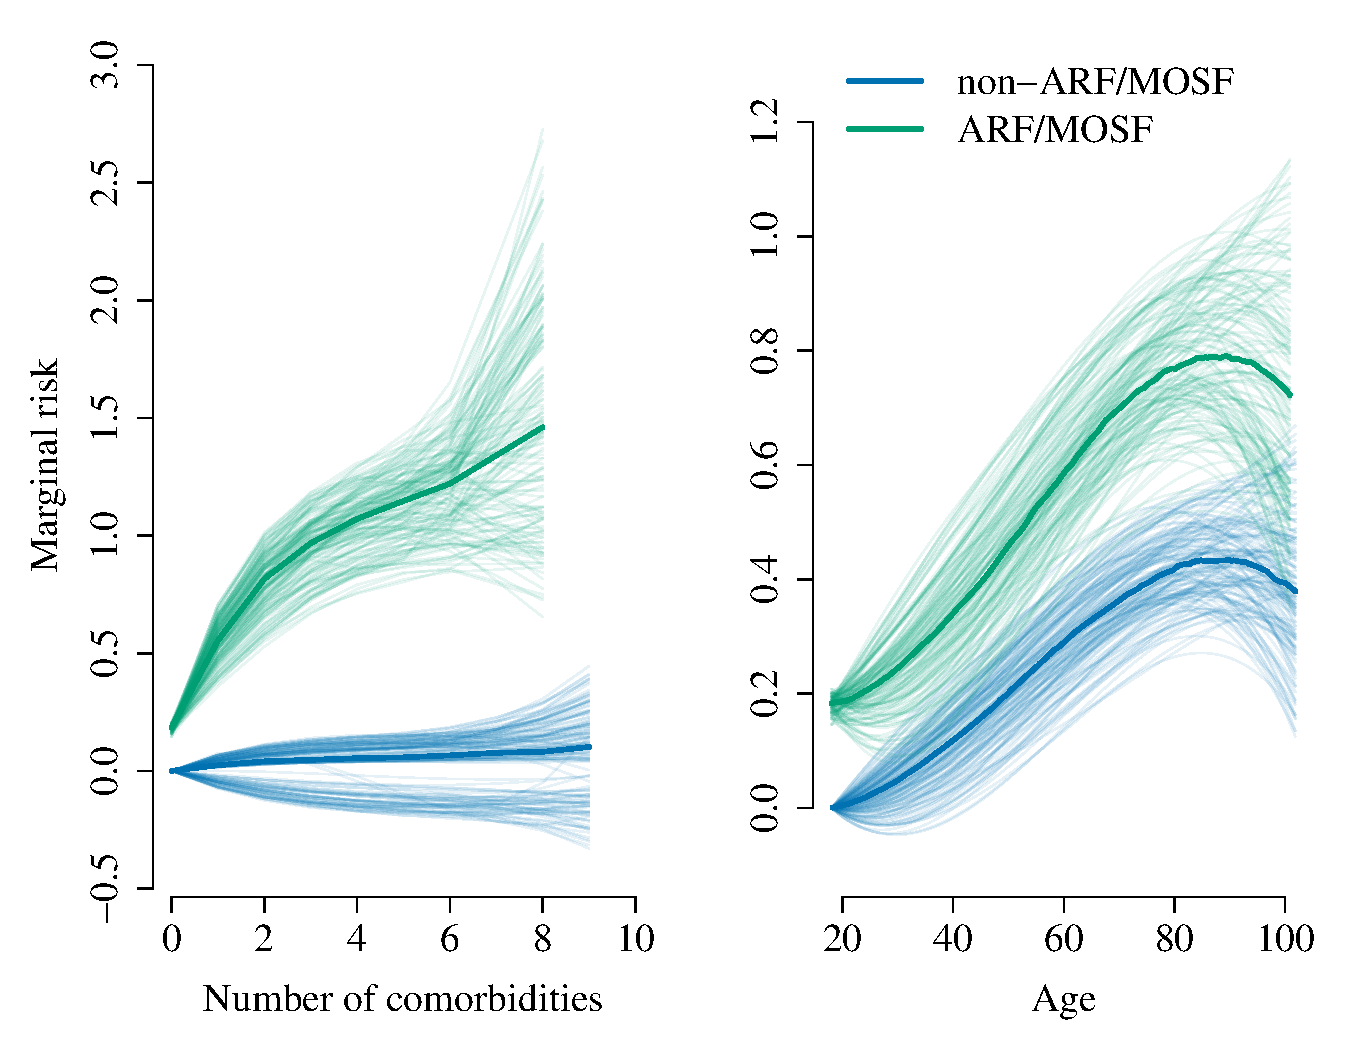
\includegraphics[width=1\linewidth]{figure/dzclass-interaction-1} 
		
	}
	
	\caption[Illustration of estimated interaction effects identified by \texttt{sail} for the SUPPORT data]{Illustration of estimated interaction effects identified by \texttt{sail} for the SUPPORT data. Median prediction curves in dark colors based on 200 train/validate/test splits represent the estimated marginal interaction effects. Coefficients estimated in each of the 200 train/validate/test splits were used to generate prediction curves representing a 90\% confidence interval colored in corresponding light colors.}\label{fig:dzclass-interaction}
\end{figure}


%\FloatBarrier



\section{Discussion} \label{sec:sail_discussion}

In this article we have introduced the sparse additive interaction learning model \sail ~for detecting non-linear interactions with a key environmental or exposure variable in high-dimensional settings.
Using a simple reparametrization, we are able to achieve either the weak or strong heredity property without using a complex penalty function. 
We developed a blockwise coordinate descent algorithm to solve the \sail ~objective function  for the least-squares loss.
We further studied the asymptotic properties of our method and showed that under certain conditions, it possesses the oracle property.
All our algorithms have been implemented in a computationally efficient, well-documented and freely available \texttt{R} package on CRAN.
Furthermore, our method is flexible enough to handle any type of basis expansion including the identity map, which allows for linear interactions.
Our implementation allows the user to selectively apply the basis expansions to the predictors, allowing for example, a combination of continuous and categorical predictors.
An extensive simulation study shows that \sail, \texttt{adaptive sail} and \texttt{sail weak} outperform existing penalized regression methods in terms of prediction accuracy, sensitivity and specificity when there are non-linear main effects only, as well as interactions with an exposure variable.
We then demonstrated the utility of our method to identify non-linear interactions in both biological and epidemiological data. 
In the NFP program, we showed that individuals who are genetically predisposed to lower educational attainment are those who stand to benefit the most from the intervention. 
Analysis of the SUPPORT data revealed that those having undergone ARF/MOSF, an increased number of comorbidities decreased their chances of survival, while there seemed to be no such relationship for non-ARF/MOSF patients. 
In a bootstrap analysis of both datasets, we observed that \sail tended to select sparser models while maintaining similar prediction performance compared to other interaction selection methods. 
%In general, we observed that \sail ~achieved similar prediction performance to other interaction selection methods, while producing much more parsimonious models. 

Our method however does have its limitations. \sail ~can currently only handle $X_E \cdot f(X)$ or $f(X_E) \cdot X$ and does not allow for $f(X, X_E)$, i.e., only one of the variables in the interaction can have a non-linear effect and we do not consider the tensor product. 
The reparametrization leads to a non-convex optimization problem which makes convergence rates difficult to assess, though we did not experience any major convergence issues in our simulations and real data analysis. 
The memory footprint can also be an issue depending on the degree of the basis expansion and the number of variables. 
Furthermore, the functional form of the covariate effects is treated as known in our method. 
Being able to automatically select for example, linear vs. nonlinear components, is currently an active area of research in main effects models~\citep{haris2016nonparametric}.
To our knowledge, our proposal is the first to allow for non-linear interactions with a key exposure variable following the weak or strong heredity property in high-dimensional settings. 
We also provide a first software implementation for these models.


\section*{Acknowledgments}

SRB and CMTG were supported by the Ludmer Centre for Neuroinformatics and Mental Health and the Canadian Institutes for Health Research PJT 148620. SRB acknowledges the support of the Natural Sciences and Engineering Research Council of Canada (NSERC), RGPIN-2020-05133.
This research was enabled in part by support provided by Calcul Québec (www.calculquebec.ca) and Compute Canada
(www.computecanada.ca). The funders had no role in study design, data collection and analysis, decision to publish, or preparation of the manuscript.


%\printcredits

%% Loading bibliography style file
%\bibliographystyle{model1-num-names}
\bibliographystyle{cas-model2-names}

% Loading bibliography database
\bibliography{sail-refs}

\newpage

\appendix

\section{Proofs} \label{ap:proofs}

As shown in the main text, we simplified the notation to make the proofs easier to follow. We summarize the original notation and the corresponding simplified notation in Table~\ref{tab:proofs}. This notation then allows us to write down the \texttt{sail} estimates as
	\begin{equation}
	\widehat{\boldsymbol{\Phi}}_{n}=\argmin_{\boldsymbol{\Phi}}Q_{n}(\boldsymbol{\Phi})=-L_{n}(\boldsymbol{\Phi})+n\lambda_{m}\sum_{m=1}^{2p+1}\left\Vert \boldsymbol{\phi}_{m}\right\Vert _{2},
	\end{equation}	
	
	\begin{table}[h]
	    \centering
	    \begin{tabular}{|c|c|c|c|c|c|c|c|c|}
	    \hline
	       $\beta_{E}^{*}$ & $\btheta_{1}^{*\top}$ & $\btheta_{2}^{*\top}$ & $\ldots$ & $\btheta_{p}^{*\top}$ & $\gamma_{1E}^{*}$ & $\gamma_{2E}^{*}$ & $\ldots$ & $\gamma_{pE}^{*}$ \\
	       \rule{0pt}{4ex}    
	       $\boldsymbol{\phi}_{1}^{*\top}$ & $\boldsymbol{\phi}_{2}^{*\top}$ & $\boldsymbol{\phi}_{3}^{*\top}$ & $\ldots$ & $\boldsymbol{\phi}_{p+1}^{*\top}$ & $\boldsymbol{\phi}_{p+2}^{*\top}$ &
	       $\boldsymbol{\phi}_{p+3}^{*\top}$ & $\ldots$ & $\boldsymbol{\phi}_{2p+1}^{*\top}$ \\
	       \midrule
	       	       \rule{0pt}{4ex}    
$\lambda(1-\alpha)w_{E}$ & $\lambda(1-\alpha)w_{2}$ & $\lambda(1-\alpha)w_{3}$ & $\ldots$ &  $\lambda(1-\alpha)w_{p+1}$ & $\lambda\alpha w_{p+2,E}$ & $\lambda\alpha w_{p+3,E}$ & $\ldots$ &  $\lambda\alpha w_{2p+1,E}$\\
	       	       \rule{0pt}{4ex}    
$\lambda_1$ & $\lambda_2$ & $\lambda_3$ & $\ldots$ & $\lambda_{p+1}$ & $\lambda_{p+2}$ & $\lambda_{p+3}$ & $\ldots$ & $\lambda_{2p+1}$ \\
	       \hline
	    \end{tabular}
	    \caption{Correspondence between parameters used to simplify the notation in the proofs. The first row shows the actual parameters used in the loss function. The second row shows the corresponding parameters in the simplified notation. The third row shows the actual tuning parameters used in the penalty function. The fourth row shows the corresponding tuning parameters in the simplified notation. This correspondence greatly simplifies the notation used in the proofs. }
	    \label{tab:proofs}
	\end{table}

\FloatBarrier
\subsection{Regularity Conditions}

\begin{description}
	\item [{(C1)}] The observation $\{\mathbf{V}_{i}:i=1\ddd n\}$ are independent
	and identically distributed with a probability density $f(\mathbf{V},\boldsymbol{\Phi})$,
	which has a common support. We assume the density $f$ satisfies the
	following equations:
	\[
	E_{\boldsymbol{\Phi}}\left[\nabla_{\boldsymbol{\phi}_{j}}\log f\left(\boldsymbol{V},\boldsymbol{\Phi}\right)\right]=\mathbf{0}\quad\text{for }j=1\ddd2p+1.
	\]
	and 
	\begin{align*}
	\mathbf{I}_{j_{1}k_{1}j_{2}k_{2}}(\boldsymbol{\Phi}) & =E_{\boldsymbol{\Phi}}\left[\frac{\partial}{\partial\phi_{j_{1}k_{1}}}\log f(V,\boldsymbol{\Phi})\cdot\frac{\partial}{\partial\phi_{j_{2}k_{2}}}\log f(V,\boldsymbol{\Phi})\right]\\
	& =E_{\boldsymbol{\Phi}}\left[-\frac{\partial^{2}}{\partial\phi_{j_{1}k_{1}}\phi_{j_{2}k_{2}}}\log f(V,\boldsymbol{\Phi})\right],
	\end{align*}
	for any $j_{1},j_{2}=1\ddd2p+1$, and $k_{1}=1\ddd p_{j1}$, $k_{2}=1\ddd p_{j2}$,
	where $j_{1},j_{2}$ are the index of group, $k_{1},k_{2}$ be the
	index of elements within the corresponding group, $p_{j_{1}},p_{j_{2}}$
	are the group size of $j_{1},j_{2}$ respectively.
	\item [{(C2)}] The Fisher information matrix 
	\[
	\mathbf{I}\left(\boldsymbol{\Phi}\right)=E\left[\left(\frac{\partial}{\partial\boldsymbol{\Phi}}\log f(V,\boldsymbol{\Phi})\right)\left(\frac{\partial}{\partial\boldsymbol{\Phi}}\log f(V,\boldsymbol{\Phi})\right)^{\top}\right]
	\]
	is finite and positive definite at $\boldsymbol{\Phi}=\boldsymbol{\Phi}^{*}$.
	\item [{(C3)}] There exists an open set $\omega$ of $\Omega$ that contains
	the true parameter point $\boldsymbol{\Phi}^{*}$ such that for almost
	all $\mathbf{V}$ the density $f(\mathbf{V},\boldsymbol{\Phi})$ admits
	all third derivatives $\frac{\partial^{3}f(\mathbf{V},\boldsymbol{\Phi})}{\partial\phi_{j_{1}k_{1}}\partial\phi_{j_{2}k_{2}}\partial\phi_{j_{3}k_{3}}}$
	for all $\boldsymbol{\Phi}$ in $\omega$ and any $j_{1},j_{2},j_{3}=1\ddd2p+1$,
	and $k_{1}=1\ddd p_{j1}$, $k_{2}=1\ddd p_{j2}$ and $k_{3}=1\ddd p_{j3}$.
	Furthermore, there exist functions $M_{j_{1}k_{1}j_{2}k_{2}j_{3}k_{3}}$
	such that
	\[
	\left|\frac{\partial^{3}}{\partial\phi_{j_{1}k_{1}}\partial\phi_{j_{2}k_{2}}\partial\phi_{j_{3}k_{3}}}\log f(\mathbf{V},\boldsymbol{\Phi})\right|\leq M_{j_{1}k_{1}j_{2}k_{2}j_{3}k_{3}}(\mathbf{V})\quad\text{for all }\boldsymbol{\Phi}\in\omega,
	\]
	and $m_{j_{1}k_{1}j_{2}k_{2}j_{3}k_{3}}=E_{\boldsymbol{\Phi}^{*}}[M_{j_{1}k_{1}j_{2}k_{2}j_{3}k_{3}}(\mathbf{V})]<\infty$.
\end{description}

\subsection{Lemma 1 proof}

{\normalsize{}Let $\eta_{n}=\frac{1}{\sqrt{n}}+a_{n}$ and $\{\boldsymbol{\Phi}^{*}+\eta_{n}\boldsymbol{\delta}:\|\boldsymbol{\delta}\|_{2}\leq C\}$
	be the ball around $\boldsymbol{\Phi}^{*}$ for $\boldsymbol{\delta}\in\mathbb{R}^{d}$,
	where $d$ is the dimension of the design matrix and $C$ is some
	constant. Under the regularity assumptions, we show that there exists
	a local minimizer $\widehat{\boldsymbol{\Phi}}_{n}$ of $Q_{n}(\boldsymbol{\Phi})$
	such that $\|\widehat{\boldsymbol{\Phi}}_{n}-\boldsymbol{\Phi}^{*}\|_{2}=O_{p}(\frac{1}{\sqrt{n}})$.
	For this proof, we adopt the approaches outlined in~\citep{fan2001variable,choi2010variable,nardi2008asymptotic,wang2007regression}
	and extend it to our situation. Let $\eta_{n}=\frac{1}{\sqrt{n}}+a_{n}$
	and $\{\boldsymbol{\Phi}^{*}+\eta_{n}\boldsymbol{\delta}:\|\boldsymbol{\delta}\|_{2}\leq C\}$
	be the ball around $\boldsymbol{\Phi}^{*}$ for $\boldsymbol{\delta}=(\mathbf{u}_{1}^{\top},\mathbf{u}_{2}^{\top},\ddd\mathbf{u}_{p+1}^{\top},\mathbf{u}_{p+2}^{\top},\ldots,\mathbf{u}_{2p+1}^{\top})^{\top}\in\mathbb{R}^{d}$,
	where $d$ is the dimension of the design matrix and $C$ is some
	constant. The objective function is given by 
	\[
	Q_{n}(\boldsymbol{\Phi})=-L_{n}(\boldsymbol{\Phi})+n\lambda_{m}\sum_{m=1}^{2p+1}\left\Vert \boldsymbol{\phi}_{m}\right\Vert _{2},
	\]
	Define
	\[
	D_{n}(\boldsymbol{\delta})\equiv Q_{n}(\boldsymbol{\Phi}^{*}+\eta_{n}\bdelta)-Q_{n}(\boldsymbol{\Phi}^{*}).
	\]
	Then for $\bdelta$ that satisfies $\|\bdelta\|_{2}=C$, we have
	\begin{align}
	D_{n}(\bdelta) & =-L_{n}(\boldsymbol{\Phi}^{*}+\eta_{n}\bdelta)+L_{n}(\boldsymbol{\Phi}^{*})+n\sum_{m=1}^{2p+1}\lambda_{m}(\|\btheta_{m}^{*}+\eta_{n}\mathbf{u}_{m}\|_{2}-\|\btheta_{m}^{*}\|_{2})\nonumber \\
	& \overset{(a)}{\geq}-L_{n}(\boldsymbol{\Phi}^{*}+\eta_{n}\bdelta)+L_{n}(\boldsymbol{\Phi}^{*})+n\sum_{m\in\mathcal{A}_{1}}\lambda_{m}(\|\btheta_{m}^{*}+\eta_{n}\mathbf{u}_{m}\|_{2}-\|\btheta_{m}^{*}\|_{2})\nonumber \\
	& \quad+n\sum_{m\in\mathcal{A}_{2}}\lambda_{m}(\|\btheta_{m}^{*}+\eta_{n}\mathbf{u}_{m}\|_{2}-\|\btheta_{m}^{*}\|_{2})\nonumber \\
	& \overset{(b)}{\geq}-L_{n}(\boldsymbol{\Phi}^{*}+\eta_{n}\bdelta)+L_{n}(\boldsymbol{\Phi}^{*})-n\eta_{n}\sum_{m\in\mathcal{A}_{1}}\lambda_{m}\|\mathbf{u}_{m}\|_{2}-n\eta_{n}\sum_{m\in\mathcal{A}_{2}}\lambda_{m}\|\mathbf{u}_{m}\|_{2}\nonumber \\
	& \overset{(c)}{\geq}-L_{n}(\boldsymbol{\Phi}^{*}+\eta_{n}\bdelta)+L_{n}(\boldsymbol{\Phi}^{*})-n\eta_{n}^{2}\sum_{m\in\mathcal{A}_{1}}\|\mathbf{u}_{m}\|_{2}-n\eta_{n}^{2}\sum_{m\in\mathcal{A}_{2}}\|\mathbf{u}_{m}\|_{2}\nonumber \\
	& \overset{}{\geq}-L_{n}(\boldsymbol{\Phi}^{*}+\eta_{n}\bdelta)+L_{n}(\boldsymbol{\Phi}^{*})-n\eta_{n}^{2}(|\A_{1}|+|\A_{2}|)C\nonumber \\
	%
	& \overset{(d)}{=}-[\nabla L_{n}(\boldsymbol{\Phi}^{*})]^{\top}(\eta_{n}\bdelta)-\frac{1}{2}(\eta_{n}\bdelta)^{\top}[\nabla^{2}L_{n}(\boldsymbol{\Phi}^{*})](\eta_{n}\bdelta)(1+o(1))\nonumber \\
	& \quad-n\eta_{n}^{2}(|\A_{1}|+|\A_{2}|)C\label{eq:lemma1}
	\end{align}
	Inequality (a) is by the fact that $\sum_{m\notin\mathcal{A}_{1}}\|\boldsymbol{\phi}_{m}^{*}\|_{2}=0$
	and $\sum_{m\notin\mathcal{A}_{2}}\|\boldsymbol{\phi}_{m}^{*}\|_{2}=0$.
	Inequality (b) is due to the reverse triangle inequality $\|a\|_{2}-\|b\|_{2}\geq-\|a-b\|_{2}$.
	Inequality (c) is by $\lambda_{m}\leq a_{n}\leq\eta_{n}$ for $m\in\A_{1}$
	and $m\in\A_{2}$ . Equality (d) is by the standard argument on the
	Taylor expansion of the loss function: 
	\begin{align*}
	L_{n}(\boldsymbol{\Phi}^{*}+\eta_{n}\bdelta) & =L_{n}(\boldsymbol{\Phi}^{*}+\eta_{n}\cdot\mathbf{0})+\eta_{n}\nabla L_{n}(\boldsymbol{\Phi}^{*}+\eta_{n}\cdot\mathbf{0})^{\top}(\bdelta-\mathbf{0})\\
	& \qquad+\frac{1}{2}(\bdelta-\mathbf{0})^{\top}\nabla^{2}L_{n}(\boldsymbol{\Phi}^{*}+\eta_{n}\cdot\mathbf{0})(\bdelta-\mathbf{0})\{1+o(1)\}\\
	& =L_{n}(\boldsymbol{\Phi}^{*})+\eta_{n}\nabla L_{n}(\boldsymbol{\Phi}^{*})^{\top}\bdelta+\frac{1}{2}\bdelta^{\top}\nabla^{2}L_{n}(\boldsymbol{\Phi}^{*})\bdelta\eta_{n}^{2}\{1+o(1)\}
	\end{align*}
	We split~\eqref{eq:lemma1} into three parts: 
	\[
	\begin{aligned}D_{1} & =-\left[\nabla L_{n}\left(\boldsymbol{\Phi}^{*}\right)\right]^{\mathrm{T}}\left(\eta_{n}\boldsymbol{\delta}\right)\\
	D_{2} & =-\frac{1}{2}\left(\eta_{n}\boldsymbol{\delta}\right)^{\top}\left[\nabla^{2}L_{n}\left(\boldsymbol{\Phi}^{*}\right)\right]\left(\eta_{n}\boldsymbol{\delta}\right)\left(1+o(1)\right)\\
	D_{3} & =-n\eta_{n}^{2}(|\A_{1}|+|\A_{2}|)C
	\end{aligned}
	\]
	Then
	\begin{align}
	D_{1} & =-\eta_{n}\left[\nabla L_{n}\left(\boldsymbol{\Phi}^{*}\right)\right]^{\top}\boldsymbol{\delta}\nonumber \\
	& =-\sqrt{n}\eta_{n}\left(\frac{1}{\sqrt{n}}\nabla L_{n}\left(\boldsymbol{\Phi}^{*}\right)\right)^{\top}\boldsymbol{\delta}\nonumber \\
	& =-\sqrt{n}\eta_{n}\left(\sqrt{n}\frac{1}{n}\sum_{i=1}^{n}\nabla\log f\left.\left(\boldsymbol{V}_{i},\boldsymbol{\Phi}\right)\right|_{\boldsymbol{\Phi}=\boldsymbol{\Phi}^{*}}\right)^{\top}\boldsymbol{\delta}\nonumber \\
	& =-\sqrt{n}\eta_{n}\left(\sqrt{n}\left[\frac{1}{n}\sum_{i=1}^{n}\nabla\log f\left.\left(\boldsymbol{V}_{i},\boldsymbol{\Phi}\right)\right|_{\boldsymbol{\Phi}=\boldsymbol{\Phi}^{*}}-\mathbf{0}\right]\right)^{\top}\boldsymbol{\delta}\nonumber \\
	& =-\sqrt{n}\eta_{n}\left(\sqrt{n}\left[\frac{1}{n}\sum_{i=1}^{n}\nabla\log f\left.\left(\boldsymbol{V}_{i},\boldsymbol{\Phi}\right)\right|_{\boldsymbol{\Phi}=\boldsymbol{\Phi}^{*}}-E_{\boldsymbol{\Phi}^{*}}\nabla L\left(\boldsymbol{\Phi}^{*}\right)\right]\right)^{\top}\boldsymbol{\delta}\nonumber \\
	& =-\sqrt{n}\eta_{n}\Op\left(1\right)\boldsymbol{\delta}\nonumber \\
	& =-\Op\left(n\eta_{n}^{2}\right)\boldsymbol{\delta}\label{eq:lemma1A1}
	\end{align}
	The last equation is by $a_{n}=o(\frac{1}{\sqrt{n}})$ and
	\begin{align*}
	\Op(n\eta_{n}^{2}) & =\Op(n(n^{-1/2}+a_{n})^{2})=\Op(1+2n^{1/2}a_{n}+na_{n}^{2}))\\
	& =\Op(1+n^{1/2}a_{n}+(n^{1/2}a_{n})^{2})=\Op(1+n^{1/2}a_{n}+o(1))\\
	& =O_{p}(n^{1/2}(n^{-1/2}+a_{n}))=O_{p}(n^{1/2}\eta_{n})
	\end{align*}
	\begin{align}
	D_{2} & =\frac{1}{2}n\eta_{n}^{2}\left\{ \boldsymbol{\delta}^{\top}\left[-\frac{1}{n}\nabla^{2}L_{n}\left(\boldsymbol{\Phi}^{*}\right)\right]\boldsymbol{\delta}\right\} \left(1+o_{p}(1)\right)\nonumber \\
	& =\frac{1}{2}n\eta_{n}^{2}\left\{ \boldsymbol{\delta}^{\top}\left[\mathbf{I}\left(\boldsymbol{\Phi}^{*}\right)\right]\boldsymbol{\delta}\right\} \left(1+o_{p}(1)\right)\text{ by the weak law of large numbers. }\nonumber \\
	& =O_{p}(n\eta_{n}^{2}\|\bdelta\|_{2}^{2})\label{eq:lemma1A2}
	\end{align}
	Combining \eqref{eq:lemma1A1} and \eqref{eq:lemma1A2} with \eqref{eq:lemma1}
	gives: 
	\[
	\begin{aligned}D_{n}(\boldsymbol{\delta}) & \geq D_{1}+D_{2}+D_{3}\\
	& =-\Op\left(n\eta_{n}^{2}\right)\boldsymbol{\delta}+O_{p}(n\eta_{n}^{2}\|\bdelta\|_{2}^{2})-n\eta_{n}^{2}(|\A_{1}|+|\A_{2}|)C
	\end{aligned}
	\]
	We can see that the first term $D_{1}$ is linear in $\bdelta$ and
	the second term $D_{2}$ is quadratic in $\bdelta$. We can conclude
	that for a large enough constant $C=\|\bdelta\|_{2}$, $D_{2}$ dominates
	$D_{1}$ and $D_{3}$. Note that this is a positive term since $I(\boldsymbol{\Phi})$
	is positive definite at $\boldsymbol{\Phi}=\boldsymbol{\Phi}^{*}$
	by regularity condition (C2). Therefore, for each $\varepsilon>0$,
	there exists a large enough constant $C$ such that, for large enough
	$n$ 
	\[
	P\left\{ \underset{\|\bdelta\|_{2}=C}{\inf}D_{n}\left(\boldsymbol{\delta}\right)>0\right\} \geq1-\varepsilon
	\]
	This implies with probability at least $1-\varepsilon$ that the empirical
	likelihood $Q_{n}$ has a local minimizer in the ball $\{\boldsymbol{\Phi}^{*}+\eta_{n}\mathbf{\bdelta}:\|\mathbf{\bdelta}\|_{2}\leq C\}$
	(since $Q_{n}$ is bounded and $\{\boldsymbol{\Phi}^{*}+\alpha_{n}\bdelta:\|\bdelta\|_{2}\leq C\}$
	is closed). In other words, there exists a local solution $\widehat{\boldsymbol{\Phi}}_{n}$
	such that $\|\widehat{\boldsymbol{\Phi}}_{n}-\boldsymbol{\Phi}^{*}\|\leq\eta_{n}\|\bdelta\|_{2}\leq\eta_{n}C=\Op(\eta_{n})=\Op(\frac{1}{\sqrt{n}}+a_{n})=O_{p}(\frac{1}{\sqrt{n}})$,
	since $a_{n}=o(\text{\ensuremath{\frac{1}{\sqrt{n}}}})$. Hence, $\left\Vert \widehat{\boldsymbol{\Phi}}_{n}-\boldsymbol{\Phi}^{*}\right\Vert _{2}=\Op\left(\frac{1}{\sqrt{n}}\right).$
	$\square$}{\normalsize\par}


\subsection{Theorem 1 proof}

{\normalsize{}We first consider consistency for the main effects
	$P\left(\widehat{\boldsymbol{\Phi}}_{\mathcal{\A}_{1}^{c}}=\mathbf{0}\right)\rightarrow1$.
	Following \citep{fan2001variable,choi2010variable}, it is sufficient
	to show that for all $m\in\A_{1}^{c}$, $P\left(\widehat{\boldsymbol{\phi}}_{m}=\mathbf{0}\right)\rightarrow1$,
	which implies that $P\left(\widehat{\boldsymbol{\Phi}}_{\mathcal{\A}_{1}^{c}}=\mathbf{0}\right)\rightarrow1$,
	i.e., the $\sqrt{n}$-consistent estimate $\widehat{\boldsymbol{\Phi}}$
	has oracle property $\widehat{\boldsymbol{\phi}}_{m}=\mathbf{0}$
	if $\boldsymbol{\phi}_{m}^{*}=\mathbf{0}$. Denote 
	\[
	\widehat{\boldsymbol{\phi}}_{m}=(\hat{\phi}_{m1}\ddd\hat{\phi}_{mp_{m}}),
	\]
	where $p_{m}$ is the group size of $\widehat{\boldsymbol{\phi}}_{m}$.
	Let $\hat{\phi}_{mk}$ be the $k$-th entry of $\widehat{\boldsymbol{\phi}}_{m}$.
	Note that if $\widehat{\boldsymbol{\phi}}_{m}\neq\mathbf{0}$, then
	$\hat{\phi}_{mk}\neq0$ for $k=1\ddd p_{m}$, then penalty function
	$\|\widehat{\boldsymbol{\phi}}_{m}\|_{2}$ becomes differentiable.
	Therefore $\phi_{mk}$ for $k=1\ddd p_{m}$ must satisfy the following
	normal equation
	\begin{align*}
	\frac{\partial Q_{n}\left(\widehat{\boldsymbol{\Phi}}_{n}\right)}{\partial\phi_{mk}}= & -\frac{\partial L_{n}\left(\widehat{\boldsymbol{\Phi}}_{n}\right)}{\partial\phi_{mk}}+n\lambda_{m}\frac{\hat{\phi}_{mk}}{\|\widehat{\boldsymbol{\phi}}_{m}\|_{2}}\\
	= & -\frac{\partial L_{n}\left(\boldsymbol{\Phi}^{*}\right)}{\partial\phi_{mk}}-\sum_{j_{1}=1}^{2p+1}\sum_{k_{1}=1}^{p_{j_{1}}}\frac{\partial^{2}L_{n}\left(\boldsymbol{\Phi}^{*}\right)}{\partial\phi_{mk}\partial\phi_{j_{1}k_{1}}}\left(\hat{\phi}_{j_{1}k_{1}}-\phi_{j_{1}k_{1}}^{*}\right)\\
	& -\frac{1}{2}\sum_{j_{1}=1}^{2p+1}\sum_{k_{1}=1}^{p_{j_{1}}}\sum_{j_{2}=1}^{2p+1}\sum_{k_{2}=1}^{p_{j_{2}}}\frac{\partial^{3}L_{n}(\widetilde{\boldsymbol{\Phi}})}{\partial\phi_{mk}\partial\phi_{j_{1}k_{1}}\partial\phi_{j_{2}k_{2}}}\left(\hat{\phi}_{j_{1}k_{1}}-\phi_{j_{1}k_{1}}^{*}\right)\left(\hat{\phi}_{j_{2}k_{2}}-\phi_{j_{2}k_{2}}^{*}\right)\\
	& +n\lambda_{m}\frac{\hat{\phi}_{mk}}{\|\widehat{\boldsymbol{\phi}}_{m}\|_{2}}\triangleq I_{1}+I_{2}+I_{3}+I_{4}=0
	\end{align*}
	where $\widetilde{\boldsymbol{\Phi}}$ lies between $\widehat{\boldsymbol{\Phi}}_{n}$
	and $\boldsymbol{\Phi}^{*}$. By the regularity conditions and Lemma
	\eqref{th:lemma1} that $\left\Vert \widehat{\boldsymbol{\Phi}}_{n}-\boldsymbol{\Phi}^{*}\right\Vert _{2}=\Op\left(\frac{1}{\sqrt{n}}\right)$,
	the first term is of the order $O_{p}(\sqrt{n})$
	\[
	I_{1}=-\frac{\partial L_{n}\left(\widehat{\boldsymbol{\Phi}}_{n}\right)}{\partial\phi_{mk}}=-\sqrt{n}\sqrt{n}\frac{1}{n}\frac{\partial L_{n}\left(\widehat{\boldsymbol{\Phi}}_{n}\right)}{\partial\phi_{mk}}=\sqrt{n}O_{p}(1)=O_{p}(\sqrt{n}).
	\]
	Then the second is of the order $\Op\left(\frac{1}{\sqrt{n}}\right)$
	and the third term is of the order $\Op\left(\frac{1}{n}\right)$.
	Hence
	\begin{align}
	\frac{\partial Q_{n}\left(\widehat{\boldsymbol{\Phi}}_{n}\right)}{\partial\boldsymbol{\Phi}_{m}}=\sqrt{n}\left\{ O_{p}(1)+\sqrt{n}\lambda_{m}\frac{\hat{\phi}_{mk}}{\|\widehat{\boldsymbol{\phi}}_{m}\|_{2}}\right\} .\label{eq:theorem1h1}
	\end{align}
	As $\sqrt{n}\lambda_{m}\geq\sqrt{n}b_{n}\to\infty$ for $m\in\mathcal{A}_{1}^{c}$
	from the assumption, therefore we know that $I_{4}$ dominates $I_{1}$,
	$I_{2}$ and $I_{3}$ in \eqref{eq:theorem1h1} with probability tending
	to one. This means that \eqref{eq:theorem1h1} cannot be true as long
	as the sample size is sufficiently large. As a result, we can conclude
	that with probability tending to one, the estimate $\widehat{\boldsymbol{\phi}}_{m}=(\hat{\phi}_{m1}\ddd\hat{\phi}_{mp_{m}})$
	must be in a position where $\widehat{\boldsymbol{\phi}}_{m}$ is
	not differentiable. Hence $\widehat{\boldsymbol{\phi}}_{m}=\mathbf{0}$
	for all $m\in\A_{1}^{c}$. Hence $P\left(\widehat{\boldsymbol{\Phi}}_{\mathcal{\A}_{1}^{c}}=\mathbf{0}\right)\rightarrow1$.
	This completes the proof. }{\normalsize\par}

{\normalsize{}Next, we prove that for the interactions $P\left(\widehat{\boldsymbol{\Phi}}_{\mathcal{\A}_{2}^{c}}=\mathbf{0}\right)\rightarrow1$.
	For $m\in\A_{2}^{c}\text{ s.t. }\text{\ensuremath{\boldsymbol{\phi}_{m}^{*}}}=\gamma_{jE}^{*}=0\text{ but }\beta_{E}\neq0\text{ and }\btheta_{j}^{*}\neq\mathbf{0}\quad(1\leq j\leq p)$,
	we can prove $P\left(\widehat{\boldsymbol{\Phi}}_{\mathcal{\A}_{2}^{c}}=\mathbf{0}\right)\rightarrow1$
	by a similar reasoning, which further implies that $P(\hat{\gamma}_{jE}=0)\rightarrow0$.
	For $m\in\A_{2}^{c}$ such that $\boldsymbol{\phi}_{m}^{*}=\gamma_{jE}^{*}=0$
	and either $\beta_{E}=0$ or $\btheta_{j}^{*}=\mathbf{0}\quad(1\leq j\leq p)$:
	without loss of generality, assume that $\btheta_{j}^{*}=\mathbf{0}$.
	Notice that $\hat{\btheta}_{j}=\mathbf{0}$ implies $\hat{\gamma}_{jE}=0$,
	since if $\hat{\gamma}_{jE}\neq0$, the value of the loss function
	does not change but the value of the penalty function will increase.
	Because we already prove $P\left(\widehat{\boldsymbol{\Phi}}_{\mathcal{\A}_{1}^{c}}=\mathbf{0}\right)\rightarrow1$,
	therefore we get $P\left(\widehat{\boldsymbol{\Phi}}_{\mathcal{\A}_{2}^{c}}=\mathbf{0}\right)\rightarrow1$
	as well for this case.}{\normalsize\par}

{\normalsize{}$\square$}{\normalsize\par}


\subsection{Theorem 2 proof}

{\normalsize{}By Lemma 1 and Theorem 1,
	there exists a $\widehat{\boldsymbol{\Phi}}_{\A}$ that is a $\sqrt{n}$-consistent
	local minimizer of $Q(\boldsymbol{\Phi}_{\A})$, therefore $\left\Vert \widehat{\boldsymbol{\Phi}}_{\A}-\boldsymbol{\Phi}_{\A}^{*}\right\Vert _{2}=\Op\left(\frac{1}{\sqrt{n}}\right)$
	and $P\left(\widehat{\boldsymbol{\Phi}}_{\mathcal{\A}^{c}}=\mathbf{0}\right)\rightarrow1$.
	Thus satisfies (with probability tending to 1): 
	\begin{equation}
	\left.\frac{\partial Q_{n}\left(\boldsymbol{\Phi}_{\A}\right)}{\partial\boldsymbol{\Phi}_{m}}\right|_{\boldsymbol{\Phi}=\left(\begin{array}{c}
		\widehat{\boldsymbol{\Phi}}_{\A}\\
		0
		\end{array}\right)}=0,\quad\forall m\in\A,\label{eq:eq_14-1}
	\end{equation}
	that is
	\begin{equation}
	\left.\frac{\partial Q_{n}\left(\boldsymbol{\Phi}_{\A}\right)}{\partial\boldsymbol{\Phi}_{m}}\right|_{\boldsymbol{\Phi}_{\A}=\widehat{\boldsymbol{\Phi}}_{\A}}=0,\quad\forall m\in\A,\label{eq:eq_14}
	\end{equation}
	where 
	\begin{align}
	Q_{n}(\boldsymbol{\Phi}_{\A}) & =-L_{n}(\boldsymbol{\Phi}_{\A})+\underbrace{n\sum_{m\in\A_{1}}\lambda_{m}\left\Vert \boldsymbol{\phi}_{m}\right\Vert _{2}+n\sum_{m\in\A_{2}}\lambda_{m}\left\Vert \boldsymbol{\phi}_{m}\right\Vert _{2}}_{\triangleq nP(\boldsymbol{\Phi}_{\A})}\nonumber \\
	& =-L_{n}(\boldsymbol{\Phi}_{\A})+nP(\boldsymbol{\Phi}_{\A}).\label{eq:eq_14.5}
	\end{align}
	From \eqref{eq:eq_14} and~\eqref{eq:eq_14.5} we have 
	\begin{equation}
	\nabla_{\A}Q_{n}\left(\widehat{\boldsymbol{\Phi}}_{\A}\right)=-\nabla_{\A}L_{n}\left(\widehat{\boldsymbol{\Phi}}_{\A}\right)+n\nabla_{\A}P\left(\widehat{\boldsymbol{\Phi}}_{\A}\right)=\mathbf{0},\label{eq:eq_15}
	\end{equation}
	with probability tending to 1.}{\normalsize\par}

{\normalsize{}Denote $\boldsymbol{\Sigma}=\diag\{o_{p}(1)\ddd o_{p}(1)\}.$
	We then expand $-\nabla_{\A}L_{n}\left(\boldsymbol{\Phi}_{\A}\right)\text{ at }\boldsymbol{\Phi}_{\A}=\boldsymbol{\Phi}_{\A}^{*}$
	in \eqref{eq:eq_15}: 
	\[
	\begin{aligned}-\nabla_{\A}L_{n}\left(\widehat{\boldsymbol{\Phi}}_{\A}\right) & =-\nabla_{\A}L_{n}\left(\boldsymbol{\Phi}_{\A}^{*}\right)-\left[\nabla_{\A}^{2}L_{n}\left(\boldsymbol{\Phi}_{\A}^{*}\right)+\boldsymbol{\Sigma}\right]\left(\widehat{\boldsymbol{\Phi}}_{\A}-\boldsymbol{\Phi}_{\A}^{*}\right)\\
	& =\sqrt{n}\left[-\frac{1}{\sqrt{n}}\nabla_{\A}L_{n}\left(\boldsymbol{\Phi}_{\A}^{*}\right)+\left(-\frac{1}{n}\nabla_{\A}^{2}L_{n}\left(\boldsymbol{\Phi}_{\A}^{*}\right)-\boldsymbol{\Sigma}\right)\sqrt{n}\left(\widehat{\boldsymbol{\Phi}}_{\A}-\boldsymbol{\Phi}_{\A}^{*}\right)\right]\\
	& =\sqrt{n}\left[-\frac{1}{\sqrt{n}}\nabla_{\A}L_{n}\left(\boldsymbol{\Phi}_{\A}^{*}\right)+\left(\mathbf{I}\left(\boldsymbol{\Phi}_{\A}^{*}\right)-\boldsymbol{\Sigma}\right)\sqrt{n}\left(\widehat{\boldsymbol{\Phi}}_{\A}-\boldsymbol{\Phi}_{\A}^{*}\right)\right].
	\end{aligned}
	\]
	The third line follows by 
	\[
	\frac{1}{n}\nabla_{\A}^{2}L_{n}\left(\boldsymbol{\boldsymbol{\Phi}}_{\A}^{*}\right)=E\left\{ \nabla_{\A}^{2}L\left(\boldsymbol{\boldsymbol{\Phi}}_{\A}^{*}\right)\right\} +\boldsymbol{\Sigma}=-\mathbf{I}\left(\boldsymbol{\boldsymbol{\Phi}}_{\A}^{*}\right)+\boldsymbol{\Sigma}.
	\]
	Denote 
	\[
	\mathbf{b}=(\lambda_{m}\textrm{sgn}\left(\beta_{m}^{*}\right),\lambda_{m}\frac{\boldsymbol{\theta}_{m}^{*}}{\|\boldsymbol{\theta}_{m}^{*}\|_{2}}^{\top},\lambda_{m}\sgn(\gamma_{mE}^{*}))^{\top},\qquad m\in\A,
	\]
	We also expand $n\nabla_{\A}P\left(\boldsymbol{\Phi}_{\A}\right)\text{ at }\boldsymbol{\Phi}_{\A}=\boldsymbol{\Phi}_{\A}^{*}$
	in \eqref{eq:eq_15}:
	\begin{align*}
	n\nabla_{\A}P\left(\widehat{\boldsymbol{\Phi}}_{\A}\right) & =n\left[\mathbf{b}+\boldsymbol{\Sigma}\left(\widehat{\boldsymbol{\Phi}}_{\A}-\boldsymbol{\Phi}_{\A}^{*}\right)\right].
	\end{align*}
	And due to the fact that $\sqrt{n}\lambda_{m}\leq\sqrt{n}a_{n}\rightarrow0$
	for $m\in\mathcal{A}$ and $\frac{\theta_{mk}^{*}}{\|\boldsymbol{\theta}_{m}^{*}\|_{2}}\leq1$
	for any $1\leq k\leq p_{m}$, we know that $\sqrt{n}\mathbf{b}=(o_{p}(1)\ddd o_{p}(1))^{\top}$
	Thus, 
	\begin{align*}
	\nabla_{\A}Q_{n}\left(\widehat{\boldsymbol{\Phi}}_{\A}\right) & =\sqrt{n}\left[-\frac{1}{\sqrt{n}}\nabla_{\A}L_{n}\left(\boldsymbol{\Phi}_{\A}^{*}\right)+\left(\mathbf{I}\left(\boldsymbol{\Phi}_{\A}^{*}\right)+\boldsymbol{\Sigma}\right)\sqrt{n}\left(\widehat{\boldsymbol{\Phi}}_{\A}-\boldsymbol{\Phi}_{\A}^{*}\right)\right]\\
	& \quad+\sqrt{n}\left[\sqrt{n}\mathbf{b}+\boldsymbol{\Sigma}\sqrt{n}\left(\widehat{\boldsymbol{\Phi}}_{\A}-\boldsymbol{\Phi}_{\A}^{*}\right)\right]\\
	& =\sqrt{n}\left[-\frac{1}{\sqrt{n}}\nabla_{\A}L_{n}\left(\boldsymbol{\Phi}_{\A}^{*}\right)+\sqrt{n}\mathbf{b}+\left(\mathbf{I}\left(\boldsymbol{\Phi}_{\A}^{*}\right)+\boldsymbol{\Sigma}\right)\sqrt{n}\left(\widehat{\boldsymbol{\Phi}}_{\A}-\boldsymbol{\Phi}_{\A}^{*}\right)\right]\\
	& =\mathbf{0}.
	\end{align*}
	\[
	\left(\mathbf{I}\left(\boldsymbol{\Phi}_{\A}^{*}\right)+\boldsymbol{\Sigma}\right)\sqrt{n}(\widehat{\boldsymbol{\Phi}}_{\A}-\boldsymbol{\Phi}_{\A}^{*})=\sqrt{n}\frac{1}{n}\sum_{i=1}^{n}\nabla_{\A}\log f\left(\boldsymbol{V}_{i},\boldsymbol{\Phi}_{\A}^{*}\right)+o_{p}(1).
	\]
	Therefore, by the central limit theorem, we know that 
	\[
	\sqrt{n}\left[\frac{1}{n}\sum_{i=1}^{n}\nabla_{\A}\log f(V_{i},\boldsymbol{\Phi}_{\A}^{*})\right]\rightarrow N(\mathbf{0},\mathbf{I}(\boldsymbol{\Phi}_{\A}^{*})).
	\]
	Hence, 
	\[
	\sqrt{n}\left(\widehat{\boldsymbol{\Phi}}_{\A}-\boldsymbol{\Phi}_{\A}^{*}\right)\overset{d}{\rightarrow}N\left(\mathbf{0},\boldsymbol{\mathbf{I}}^{-1}\left(\boldsymbol{\Phi}_{\A}^{*}\right)\right).
	\]
	}{\normalsize{}$\square$}{\footnotesize\par}


\section{Algorithm Details} \label{ap:sail_algorithm}

In this section we provide more specific details about the algorithms used to solve the \sail ~objective function. We assume that $Y$, $\bPsi_j$, $X_E$ and $X_E \circ \bPsi_j$ have been centered by their sample means $\widebar{Y}$, $\widebar{\bPsi}_j$, $\widebar{X}_E$, and $\widebar{X_E \circ \bPsi_j}$, respectively. Here, $\widebar{\bPsi}_j \in \mathbb{R}^{m_j}$ and $\widebar{X_E \circ \bPsi_j}\in \mathbb{R}^{m_j}$  represent the column means of $\bPsi_j$ and $X_E \circ \bPsi_j$, respectively. Since the intercept ($\beta_0$) is not penalized and all variables have been centered, we can omit it from the loss function and  compute it once the algorithm has converged for all other parameters. The strong heredity \texttt{sail} model with least-squares loss has the form
\begin{equation}
\hat{Y}   =   \sum_{j=1}^p \bPsi_j \btheta_j + \beta_E X_E + \sum_{j=1}^p \gamma_{j}  \beta_E (X_E \circ \bPsi_j) \btheta_j
\end{equation}
and the objective function is given by
\begin{equation}
Q(\bPhi) = \frac{1}{2n} \norm{Y - \hat{Y}}_2^2 + \lambda (1-\alpha)  \left( w_E \abs{\beta_E} + \sum_{j=1}^{p} w_j \norm{\btheta_j}_2 \right) +  \lambda\alpha \sum_{j=1}^{p} w_{jE} \abs{\gamma_{j}} \label{eq:objective_least-squares}
\end{equation}

Solving~\eqref{eq:objective_least-squares} in a blockwise manner allows us to leverage computationally fast algorithms for $\ell_1$ and $\ell_2$ norm penalized regression.
Denote the $n$-dimensional residual column vector $R = Y-\hat{Y}$. The subgradient equations are given by
\begin{align}
%\frac{\partial Q}{\partial \beta_0} & = \frac{1}{n} \left( Y - \beta_0 \cdot \boldsymbol{1} - \sum_{j=1}^p \bPsi_j \btheta_j - \beta_E X_E - \sum_{j=1}^p \gamma_{j}  \beta_E (X_E \circ \bPsi_j) \btheta_j\right)^\top \boldsymbol{1}  = 0 \label{eq:sub_b0} \\
\frac{\partial Q}{\partial \beta_E} & = -\frac{1}{n} \left(X_E + \sum_{j=1}^{p}\gamma_j (X_E \circ \bPsi_j)\btheta_j\right)^\top R  + \lambda (1-\alpha) w_E s_1 = 0 \label{eq:sub_bE}\\
\frac{\partial Q}{\partial \btheta_j} & = -\frac{1}{n} \left(\bPsi_j + \gamma_j \beta_E (X_E \circ \bPsi_j)\right)^\top R  + \lambda (1-\alpha) w_j s_2 = \boldsymbol{0} \label{eq:sub_thetaj}\\
\frac{\partial Q}{\partial \gamma_j} & = -\frac{1}{n} \left(\beta_E (X_E \circ \bPsi_j)\btheta_j\right)^\top R  + \lambda \alpha w_{jE} s_3 = 0 \label{eq:sub_gammaj}
\end{align}
where $s_1$ is in the subgradient of the $\ell_1$ norm:
$$
s_1 \in \begin{cases}
\textrm{sign}\left(\beta_E\right) & \tm{if  } \beta_E \neq 0\\
[-1, 1] &  \tm{if  } \beta_E = 0,\\
\end{cases}
$$
$s_2$ is in the subgradient of the $\ell_2$ norm:
$$
s_2 \in \begin{cases}
\dfrac{\btheta_j}{\norm{\btheta_j}_2} &  \tm{if  } \btheta_j \neq \boldsymbol{0}\\
u \in \mathbb{R}^{m_j}: \norm{u}_2 \leq 1 & \tm{if  } \btheta_j = \boldsymbol{0},\\
\end{cases}
$$
and $s_3$ is in the subgradient of the $\ell_1$ norm:
$$
s_3 \in \begin{cases}
\textrm{sign}\left(\gamma_j\right) & \tm{if  } \gamma_j \neq 0\\
[-1, 1] &  \tm{if  } \gamma_j = 0.\\
\end{cases}
$$
Define the partial residuals, without the $j$th predictor for $j=1, \ldots, p$, as
\[R_{(-j)} = Y -  \sum_{\ell \neq j} \bPsi_\ell \btheta_\ell - \beta_E X_E - \sum_{\ell\neq j} \gamma_{\ell}  \beta_E (X_E \circ \bPsi_\ell) \btheta_\ell \]
the partial residual without $X_E$ as
\[R_{(-E)} = Y  - \sum_{j=1}^p \bPsi_j \btheta_j\]
and the partial residual without the $j$th interaction for $j=1, \ldots, p$, as
\[R_{(-jE)} = Y  - \sum_{j=1}^p \bPsi_j \btheta_j - \beta_E X_E - \sum_{\ell\neq j} \gamma_{\ell}  \beta_E (X_E \circ \bPsi_\ell) \btheta_\ell \]
From the subgradient equations~\eqref{eq:sub_bE}--\eqref{eq:sub_gammaj} we see that
\begin{align}
&\hat{\beta}_E  = \frac{S\left(\frac{1}{n \cdot w_E}\left(X_E + \sum_{j=1}^{p}\hat\gamma_j (X_E \circ \bPsi_j)\hat\btheta_j\right)^\top R_{(-E)} , \lambda(1-\alpha)\right)}{\left(X_E + \sum_{j=1}^{p}\hat\gamma_j (X_E \circ \bPsi_j)\hat\btheta_j\right)^\top\left(X_E + \sum_{j=1}^{p}\hat\gamma_j (X_E \circ \bPsi_j)\hat\btheta_j\right)} \label{eq:betaE} \\
&\lambda (1-\alpha) w_j \dfrac{\btheta_j}{\norm{\btheta_j}_2}  =  \frac{1}{n} \left(\bPsi_j + \gamma_j \beta_E (X_E \circ \bPsi_j)\right)^\top R_{(-j)} \label{eq:thetaj} \\
&\hat\gamma_j  = \frac{S \left(\frac{1}{n \cdot w_{jE}}\left(\beta_E (X_E \circ \bPsi_j)\btheta_j\right)^\top R_{(-jE)}, \lambda \alpha\right)}{\left(\beta_E (X_E \circ \bPsi_j)\btheta_j\right)^\top\left(\beta_E (X_E \circ \bPsi_j)\btheta_j\right)} \label{eq:gammaj}
\end{align}
where $S(x,t) = \textrm{sign}(x) (\abs{x} - t)$ is the soft-thresholding operator. Given these estimates, the intercept can be computed using the following equation:
\begin{equation}
\hat{\beta}_0 =   \widebar{Y} - \sum_{j=1}^p \widebar{\bPsi}_j \hat\btheta_j - \hat\beta_E \widebar{X}_E - \sum_{j=1}^p \hat\gamma_{j}  \hat\beta_E (\widebar{X_E \circ \bPsi_j}) \hat\btheta_j. \label{eq:beta0} \\
\end{equation}
We see from~\eqref{eq:betaE} that there is a closed form solution for $\beta_E$. From~\eqref{eq:gammaj}, each $\gamma_j$ also has a closed form solution and can be solved efficiently for $j=1, \ldots, p$ using a coordinate descent procedure~\citep{friedman2010regularization}.
Since there is no closed form solution for $\beta_j$, we use a quadratic majorization technique~\citep{yang2015fast} to solve~\eqref{eq:thetaj}. Furthermore, we update each $\btheta_{j}$ in a coordinate wise fashion and leverage this to implement further computational speedups which are detailed in Supplemental Section~\ref{ap:subsec:Delta}.
From these estimates, we compute the interaction effects using the reparametrizations presented in Table~\ref{tab:reparam}, e.g.,  $\hat{\btau}_j = \hat{\gamma}_j \hat{\beta}_E \hat{\btheta}_j$, $j=1, \ldots, p$ for the strong heredity \sail ~model.


\subsection{Least-Squares \sail ~with Strong Heredity} \label{ap:subsec:lssail}
A more detailed algorithm for fitting the least-squares \texttt{sail} model with strong heredity is given in Algorithm~\ref{alg:lssail}.
\begin{algorithm}
	\caption{Blockwise Coordinate Descent for Least-Squares \texttt{sail} with Strong Heredity}\label{alg:lssail}
	\begin{algorithmic}[1]
		%\algsetup{linenosize=\tiny}
		\small
		\Function{\texttt{sail}}{$\boldsymbol{X},Y, X_E,\texttt{basis},\lambda, \alpha,w_j, w_E, w_{jE}, \epsilon$}\Comment{Algorithm for solving~\eqref{eq:objective_least-squares}}
		%\State $\Psi_j \gets $ \texttt{splines::bs}($X_j$, \texttt{df}, \texttt{degree}) for $j=1, \ldots, p$
		%\State $\widetilde\Psi_j \gets X_E \circ \Psi_j$ for $j=1, \ldots, p$
		\State $\bPsi_j \gets $ \texttt{basis}($X_j$), $\widetilde{\bPsi}_j \gets X_E \circ \bPsi_j$ for $j=1, \ldots, p$
		%\item[]
		\State Center all variables by their sample means
		\State Initialize: $\beta_E^{(0)}=\btheta_j^{(0)}=\gamma_j^{(0)} \gets 0$ for $j=1, \ldots, p$.
		%\State Initialize: $R^\ast \gets Y $ %\Comment{Initial partial residual used for $\btheta$ update}
		\State Set iteration counter $k \gets 0$
		\State $R^\ast \gets Y - \beta_E^{(k)} X_E - \sum_{j}  (\bPsi_{j} + \gamma_{j}^{(k)} \beta_E^{(k)}  \widetilde{\bPsi}_{j}) \btheta_{j}^{(k)}$
		\Repeat
		\State $\bullet$ To update $\boldsymbol{\gamma}=(\gamma_1, \ldots, \gamma_p)$
		\Indent
		\State $\widetilde{X}_j \gets \beta_E^{(k)} \widetilde{\bPsi}_j \btheta_j^{(k)} \qquad$ for $j = 1, \ldots, p$
		\State $R \gets R^\ast + \sum_{j=1}^p  \gamma_{j}^{(k)} \widetilde{X}_j$
		%\State $R_1 \gets Y - \beta_0^{(k)} - \beta_E^{(k)} X_E - \sum_{j} \bPsi_j \btheta_j^{(k)}$
		\State \[\boldsymbol{\gamma}^{(k)(new)} \gets \argmin_{\boldsymbol{\gamma}} \frac{1}{2n} \norm{R - \sum_{j} \gamma_j \widetilde{X}_j}_2^2 + \lambda \alpha \sum_{j} w_{jE} \abs{\gamma_{j}}\]
		\State $\Delta = \sum_j (\gamma_j^{(k)} - \gamma_j^{(k)(new)}) \widetilde{X}_j $
		\State $R^\ast \gets R^\ast + \Delta$
		\EndIndent
		\State $\bullet$ To update $\btheta = (\btheta_1, \ldots, \btheta_p)$
		\Indent
		\State %$\beta_0^{(k)} \gets \beta_0^{(k-1)}$, $\btheta_j^{(k)} \gets \btheta_j^{(k-1)}$,
		$\widetilde{X}_j \gets \bPsi_j + \gamma_{j}^{(k)} \beta_E^{(k)} \widetilde{\bPsi}_{j}$ for $j=1, \ldots, p$
		\For{$j=1, \ldots, p$}
		\State $R \gets R^\ast + \widetilde{X}_j\btheta_j^{(k)}$
		%\State $R_2 \gets Y - \beta_0^{(k)} - \beta_E^{(k)} X_E - \sum_{j=1}^p  (\bPsi_{j} + \gamma_{j}^{(k)} \beta_E^{(k)}  \widetilde{\bPsi}_{j}) \btheta_{j}^{(k)} + (\bPsi_j + \gamma_j^{(k)}\beta_E^{(k)} \widetilde{\bPsi}_j)\btheta_j^{(k)}$
		%\If{$j=1$} \State $\Delta \gets 0$ \Else \State $\Delta \gets \widetilde{X}_{j}  \btheta_{j}^{(k)} - \widetilde{X}_{j-1} \btheta_{j-1}^{(k)}$ \Comment{see~\eqref{subsec:Delta} for details}
		%\EndIf
		%\State $R_2 \gets R_2 + \Delta$
		\State \[\btheta_j^{(k)(new)} \gets \argmin_{\btheta_j} \frac{1}{2n} \norm{R -  \widetilde{X}_j \btheta_j}_2^2 + \lambda (1-\alpha) w_j \norm{\theta_j}_2\]
		%\State $R_2^{\prime\prime} \gets Y - \beta_0^{(k)} - \beta_E^{(k)} X_E - \sum_{\ell \neq j}  \bPsi_{\ell} \btheta_{\ell}^{(k)} - \sum_{\ell \neq j} \gamma_{\ell}^{(k)} \beta_E^{(k)}  \widetilde{\bPsi}_{\ell} \btheta_{\ell}^{(k)} $
		\State $\Delta = \widetilde{X}_j(\btheta_j^{(k)} - \btheta_j^{(k)(new)})$
		\State $R^\ast \gets R^\ast + \Delta$
		\EndFor
		\EndIndent
		%\item[]
		\State $\bullet$ To update $\beta_E$
		\Indent
		\State $\widetilde{X}_E \gets X_E + \sum_{j} \gamma_j^{(k)} \widetilde{\bPsi}_j \btheta_j^{(k)}$
		%\State $R \gets R^\ast + \beta_E^{(k)} X_E + \sum_{j}  ( \gamma_{j}^{(k)} \beta_E^{(k)}  \widetilde{\bPsi}_{j}) \btheta_{j}^{(k)} = R^\ast + \beta_E^{(k)} \widetilde{X}_E$
		\State $R \gets R^\ast + \beta_E^{(k)} \widetilde{X}_E$
		%\State $R_3 \gets Y - \beta_0^{(k)} - \sum_j \bPsi_j \btheta_j^{(k)} - \sum_{j} \gamma_j^{(k)}  \bPsi_j \btheta_j^{(k)}$
		\State \[\beta_E^{(k)(new)} \gets \frac{1}{ \widetilde{X}_E^\top\widetilde{X}_E}S\left(\frac{1}{n \cdot w_E} \widetilde{X}_E^\top R, \lambda(1-\alpha)\right)\] \Comment{$S(x,t) = \textrm{sign}(x) (\abs{x} - t)_+$}
		%\State $\beta_E^{(k)} \gets \argmin_{\beta_E} \frac{1}{2n} \norm{R_3 - \beta_E \widetilde{X}_E}_2^2 + \lambda(1-\alpha) w_E \abs{\beta_E}$
		\State $\Delta = (\beta_E^{(k)} - \beta_E^{(k)(new)})\widetilde{X}_E$
		\State $R^\ast \gets R^\ast + \Delta$
		\EndIndent
		%\State $\bullet$ To update $\beta_0$
		%\Indent
		%\State $R \gets R^* + \beta_0^{(k)}$
		%\State $R_4 \gets Y - \beta_E^{(k)} X_E - \sum_{j}  \bPsi_{j} \btheta_{j}^{(k)} - \sum_{j} \gamma_{j}^{(k)} \beta_E^{(k)}  \widetilde{\bPsi}_{j} \btheta_{j}^{(k)}$
		%\State \[\beta_0^{(k)(new)} \gets \frac{1}{n} R \cdot \boldsymbol{1}\]
		%\State $\Delta = \beta_0^{(k)} - \beta_0^{(k)(new)}$
		%\State $R^\ast \gets R^\ast + \Delta$
		%\EndIndent
		\State $k \gets k + 1$
		%\State \Until{convergence criterion is satisfied: $\norm{\bPhi^{(k)} - \bPhi^{(k-1)}}_2^2 < \epsilon$}
		\State \Until{convergence criterion is satisfied: $\abs{Q(\bPhi^{(k-1)}) - Q(\bPhi^{(k)})} /Q(\bPhi^{(k-1)})  < \epsilon$}
		\State Compute the intercept $\beta_0$
		\Indent
		\State $\beta_0 \gets \widebar{Y} - \sum_{j=1}^p \widebar{\bPsi}_j \hat\btheta_j - \hat\beta_E \widebar{X}_E - \sum_{j=1}^p \hat\gamma_{j}  \hat\beta_E (\widebar{X_E \circ \bPsi_j}) \hat\btheta_j$
		\EndIndent
		\EndFunction
	\end{algorithmic}
\end{algorithm}

\newpage


\subsection{Details on Update for $\btheta$} \label{ap:subsec:Delta}

Here we discuss a computational speedup in the updates for the $\btheta$ parameter. The partial residual ($R_{s}$) used for updating $\btheta_s$ ($s \in {1,\ldots, p}$) at the $k$th iteration is given by
\begin{align}
R_{s} & = Y - \widetilde{Y}_{(-s)}^{(k)} \label{eq:r2}
\end{align}
where $\widetilde{Y}_{(-s)}^{(k)}$ is the fitted value at the $k$th iteration excluding the contribution from $\bPsi_s$:
\begin{align}
\widetilde{Y}_{(-s)}^{(k)} & = \beta_E^{(k)} X_E + \sum_{\ell \neq s}  \bPsi_{\ell} \btheta_{\ell}^{(k)} + \sum_{\ell \neq s} \gamma_{\ell}^{(k)} \beta_E^{(k)}  \widetilde{\bPsi}_{\ell} \btheta_{\ell}^{(k)} \label{eq:r2_2}
\end{align}
Using~\eqref{eq:r2_2},~\eqref{eq:r2} can be re-written as
\begin{align}
% R_2 & = Y - \beta_0^{(k)} - \beta_E^{(k)} X_E - \sum_{j=1}^p  \bPsi_{j} \btheta_{j}^{(k)} - \sum_{j=1}^p \gamma_{j}^{(k)} \beta_E^{(k)}  \widetilde{\bPsi}_{j} \btheta_{j}^{(k)} + (\bPsi_s + \gamma_s^{(k)}\beta_E^{(k)} \widetilde{\bPsi}_s)\btheta_s^{(k)}  \\
R_{s} & = Y -  \beta_E^{(k)} X_E - \sum_{j=1}^p  (\bPsi_{j} + \gamma_{j}^{(k)} \beta_E^{(k)}  \widetilde{\bPsi}_{j}) \btheta_{j}^{(k)} + (\bPsi_s + \gamma_s^{(k)}\beta_E^{(k)} \widetilde{\bPsi}_s)\btheta_s^{(k)} \nonumber \\
& = R^\ast + (\bPsi_s + \gamma_s^{(k)}\beta_E^{(k)} \widetilde{\bPsi}_s)\btheta_s^{(k)} \label{eq:r2_3}
\end{align}
where
\begin{equation}
R^\ast = Y - \beta_E^{(k)} X_E - \sum_{j=1}^p  (\bPsi_{j} + \gamma_{j}^{(k)} \beta_E^{(k)}  \widetilde{\bPsi}_{j}) \btheta_{j}^{(k)} \label{eq:rast}
\end{equation}
Denote $\btheta_{s}^{(k)(\tm{new})}$ the solution for predictor $s$ at the $k$th iteration, given by:
\begin{align}
\btheta_s^{(k)(new)} = \argmin_{\btheta_j} \frac{1}{2n} \norm{R_s - (\bPsi_s + \gamma_{s}^{(k)} \beta_E^{(k)}\widetilde{\bPsi}_{s})\btheta_j }_2^2 + \lambda (1-\alpha) w_s \norm{\theta_j}_2 \label{eq:r2_4}
\end{align}
Now we want to update the parameters for the next predictor $\btheta_{s+1}$ ($s+1 \in {1,\ldots, p}$) at the $k$th iteration. The partial residual used to update $\btheta_{s+1}$ is given by
\begin{align}
R_{s+1} & = R^\ast + (\bPsi_{s+1} + \gamma_{s+1}^{(k)}\beta_E^{(k)} \widetilde{\bPsi}_{s+1})\btheta_{s+1}^{(k)} + (\bPsi_s + \gamma_s^{(k)}\beta_E^{(k)} \widetilde{\bPsi}_s)(\btheta_s^{(k)} - \btheta_s^{(k)(new)}) \label{eq:r2_5}
\end{align}
where $R^\ast$ is given by~\eqref{eq:rast}, $\btheta_s^{(k)}$ is the parameter value prior to the update, and $\btheta_s^{(k)(new)}$ is the updated value given by~\eqref{eq:r2_4}. Taking the difference between~\eqref{eq:r2_3} and~\eqref{eq:r2_5} gives
\begin{align}
\Delta & = R_t - R_s \nonumber\\
& = (\bPsi_t + \gamma_t^{(k)}\beta_E^{(k)} \widetilde{\bPsi}_t)\btheta_t^{(k)} + (\bPsi_s + \gamma_s^{(k)}\beta_E^{(k)} \widetilde{\bPsi}_s)(\btheta_s^{(k)} - \btheta_s^{(k)(new)}) - (\bPsi_s + \gamma_s^{(k)}\beta_E^{(k)} \widetilde{\bPsi}_s)\btheta_s^{(k)} \nonumber\\
& = (\bPsi_t + \gamma_t^{(k)}\beta_E^{(k)} \widetilde{\bPsi}_t)\btheta_t^{(k)} - (\bPsi_s + \gamma_s^{(k)}\beta_E^{(k)} \widetilde{\bPsi}_s)\btheta_s^{(k)(new)} \label{eq:Delta}
\end{align}
Therefore $R_t = R_s + \Delta$, and the partial residual for updating the next predictor can be computed by updating the previous partial residual by $\Delta$, given by~\eqref{eq:Delta}. This formulation can lead to computational speedups especially when $\Delta = 0$, meaning the partial residual does not need to be re-calculated.

\subsection{Maximum penalty parameter ($\lambda_{max}$) for strong heredity}

The subgradient equations~\eqref{eq:sub_bE}--\eqref{eq:sub_gammaj} can be used to determine the largest value of $\lambda$ such that all coefficients are 0. From the subgradient Equation~\eqref{eq:sub_bE}, we see that $\beta_E = 0$ is a solution if
\begin{equation}
\frac{1}{w_E}\abs{\frac{1}{n} \left(X_E + \sum_{j=1}^{p}\gamma_j (X_E \circ \bPsi_j)\btheta_j\right)^\top R_{(-E)}} \leq \lambda (1-\alpha)
\end{equation}
From the subgradient Equation~\eqref{eq:sub_thetaj}, we see that $\btheta_j = \boldsymbol{0}$ is a solution if
\begin{equation}
\frac{1}{w_{j}}\norm{\frac{1}{n} \left(\bPsi_j + \gamma_j \beta_E (X_E \circ \bPsi_j)\right)^\top R_{(-j)}}_2 \leq \lambda (1-\alpha)
\end{equation}
From the subgradient Equation~\eqref{eq:sub_gammaj}, we see that $\gamma_j = 0$ is a solution if
\begin{equation}
\frac{1}{w_{jE}}\abs{\frac{1}{n} \left(\beta_E (X_E \circ \bPsi_j)\btheta_j\right)^\top R_{(-jE)}} \leq \lambda \alpha
\end{equation}
Due to the strong heredity property, the parameter vector $(\beta_E,\btheta_1, \ldots, \btheta_p, \gamma_1, \ldots, \gamma_p)$ will be entirely equal to $\boldsymbol{0}$ if $(\beta_E,\btheta_1, \ldots, \btheta_p) = \boldsymbol{0}$. Therefore, the smallest value of $\lambda$ for which the entire parameter vector (excluding the intercept) is $\boldsymbol{0}$ is:
\begin{multline}
\lambda_{max} = \frac{1}{n(1-\alpha)} \max \left\lbrace \frac{1}{w_E}\left(X_E + \sum_{j=1}^{p}\gamma_j (X_E \circ \bPsi_j)\btheta_j\right)^\top R_{(-E)}, \right. \\
\left. \max_j \frac{1}{w_{j}}\norm{\left(\bPsi_j + \gamma_j \beta_E (X_E \circ \bPsi_j)\right)^\top R_{(-j)}}_2   \right\rbrace
\end{multline}
which reduces to
\begin{align*}
\lambda_{max} = \frac{1}{n(1-\alpha)} \max \left\lbrace \frac{1}{w_E}\left(X_E\right)^\top R_{(-E)}, \max_j \frac{1}{w_{j}}\norm{\left(\bPsi_j\right)^\top R_{(-j)}}_2   \right\rbrace
\end{align*}

\subsection{Least-Squares \sail ~with Weak Heredity} \label{ap:subsec:lssailweak}

We assume the same centering constraints as in Section~\ref{ap:subsec:lssail}. The least-squares \texttt{sail} model with weak heredity has the form
\begin{equation}
\hat{Y}   =   \sum_{j=1}^p \bPsi_j \btheta_j + \beta_E X_E + \sum_{j=1}^p \gamma_{j}  (X_E \circ \bPsi_j) (\beta_E\cdot \mb{1}_{m_j} + \btheta_j)
\end{equation}
The objective function is given by
\begin{equation}
Q(\bPhi) = \frac{1}{2n} \norm{Y - \hat{Y}}_2^2 + \lambda (1-\alpha)  \left( w_E \abs{\beta_E} + \sum_{j=1}^{p} w_j \norm{\btheta_j}_2 \right) +  \lambda\alpha \sum_{j=1}^{p} w_{jE} \abs{\gamma_{j}} \label{eq:objective_least-squares-weak}
\end{equation}
Denote the $n$-dimensional residual column vector $R = Y-\hat{Y}$. The subgradient equations are given by
\begin{align}
\frac{\partial Q}{\partial \beta_E} & = -\frac{1}{n} \left(X_E + \sum_{j=1}^{p}\gamma_j (X_E \circ \bPsi_j)\mb{1}_{m_j}\right)^\top R  + \lambda (1-\alpha) w_E s_1 = 0 \label{eq:sub_bEweak}\\
\frac{\partial Q}{\partial \btheta_j} & = -\frac{1}{n} \left(\bPsi_j + \gamma_j (X_E \circ \bPsi_j)\right)^\top R  + \lambda (1-\alpha) w_j s_2 = \boldsymbol{0} \label{eq:sub_thetajweak}\\
\frac{\partial Q}{\partial \gamma_j} & = -\frac{1}{n} \left((X_E \circ \bPsi_j)(\beta_E \cdot \mb{1}_{m_j} + \btheta_j)\right)^\top R  + \lambda \alpha w_{jE} s_3 = 0 \label{eq:sub_gammajweak}
\end{align}
where $s_1$ is in the subgradient of the $\ell_1$ norm:
$$
s_1 \in \begin{cases}
\textrm{sign}\left(\beta_E\right) & \tm{if  } \beta_E \neq 0\\
[-1, 1] &  \tm{if  } \beta_E = 0,\\
\end{cases}
$$
$s_2$ is in the subgradient of the $\ell_2$ norm:
$$
s_2 \in \begin{cases}
\dfrac{\btheta_j}{\norm{\btheta_j}_2} &  \tm{if  } \btheta_j \neq \boldsymbol{0}\\
u \in \mathbb{R}^{m_j}: \norm{u}_2 \leq 1 & \tm{if  } \btheta_j = \boldsymbol{0},\\
\end{cases}
$$
and $s_3$ is in the subgradient of the $\ell_1$ norm:
$$
s_3 \in \begin{cases}
\textrm{sign}\left(\gamma_j\right) & \tm{if  } \gamma_j \neq 0\\
[-1, 1] &  \tm{if  } \gamma_j = 0.\\
\end{cases}
$$
Define the partial residuals, without the $j$th predictor for $j=1, \ldots, p$, as
\[R_{(-j)} = Y  - \sum_{\ell \neq j} \bPsi_\ell \btheta_\ell - \beta_E X_E - \sum_{\ell\neq j} \gamma_{\ell}  (X_E \circ \bPsi_\ell) (\beta_E \cdot \mb{1}_{m_{\ell}} +\btheta_\ell) \]
the partial residual without $X_E$ as
\[R_{(-E)} = Y  - \sum_{j=1}^p \bPsi_j \btheta_j - \sum_{j=1}^p \gamma_{j}  (X_E \circ \bPsi_j) \btheta_j\]
and the partial residual without the $j$th interaction for $j=1, \ldots, p$
\[R_{(-jE)} = Y  - \sum_{j=1}^p \bPsi_j \btheta_j - \beta_E X_E - \sum_{\ell\neq j} \gamma_{\ell} (X_E \circ \bPsi_\ell) (\beta_E \cdot \mb{1}_{m_{\ell}} +\btheta_\ell) \]
From the subgradient Equation~\eqref{eq:sub_bEweak}, we see that $\beta_E = 0$ is a solution if
\begin{equation}
\frac{1}{w_E}\abs{\frac{1}{n} \left(X_E + \sum_{j=1}^{p}\gamma_j (X_E \circ \bPsi_j)\mb{1}_{m_j}\right)^\top R_{(-E)}} \leq \lambda (1-\alpha)
\end{equation}
From the subgradient Equation~\eqref{eq:sub_thetajweak}, we see that $\btheta_j = \boldsymbol{0}$ is a solution if
\begin{equation}
\frac{1}{w_{j}}\norm{\frac{1}{n} \left(\bPsi_j + \gamma_j (X_E \circ \bPsi_j)\right)^\top R_{(-j)}}_2 \leq \lambda (1-\alpha)
\end{equation}
From the subgradient Equation~\eqref{eq:sub_gammajweak}, we see that $\gamma_j = 0$ is a solution if
\begin{equation}
\frac{1}{w_{jE}}\abs{\frac{1}{n} \left((X_E \circ \bPsi_j)(\beta_E \cdot \mb{1}_{m_j}+\btheta_j)\right)^\top R_{(-jE)}} \leq \lambda \alpha
\end{equation}
From the subgradient equations we see that
\begin{align}
%&\hat{\beta}_0 =  \left( Y - \sum_{j=1}^p \bPsi_j \hat\btheta_j - \hat\beta_E X_E - \sum_{j=1}^p \hat\gamma_{j}   (X_E \circ \bPsi_j)(\hat\beta_E\cdot \mb{1}_{m_j}+ \hat\btheta_j)\right)^\top \boldsymbol{1} \\
&\hat{\beta}_E  = \frac{S\left(\frac{1}{n\cdot w_E}\left(X_E + \sum_{j=1}^{p}\hat\gamma_j (X_E \circ \bPsi_j)\mb{1}_{m_j}\right)^\top R_{(-E)}, \lambda(1-\alpha)\right)}{\left(X_E + \sum_{j=1}^{p}\hat\gamma_j (X_E \circ \bPsi_j)\mb{1}_{m_j}\right)^\top\left(X_E + \sum_{j=1}^{p}\hat\gamma_j (X_E \circ \bPsi_j)\mb{1}_{m_j}\right)} \\
&\lambda (1-\alpha) w_j \dfrac{\btheta_j}{\norm{\btheta_j}_2}  =  \frac{1}{n} \left(\bPsi_j + \gamma_j (X_E \circ \bPsi_j)\right)^\top R_{(-j)} \label{eq:thetajweak} \\
&\hat\gamma_j  = \frac{ S \left(\frac{1}{n \cdot w_{jE}}  \left((X_E \circ \bPsi_j)(\beta_E \cdot \mb{1}_{m_j}+\btheta_j)\right)^\top R_{(-jE)}, \lambda \alpha\right)}{\left((X_E \circ \bPsi_j)(\beta_E \cdot \mb{1}_{m_j}+\btheta_j)\right)^\top \left((X_E \circ \bPsi_j)(\beta_E \cdot \mb{1}_{m_j}+\btheta_j)\right)}
\end{align}
where $S(x,t) = \textrm{sign}(x) (\abs{x} - t)$ is the soft-thresholding operator. As was the case in the strong heredity \sail ~model, there is a closed form solution for $\beta_E$, each $\gamma_j$ also has a closed form solution and can be solved efficiently for $j=1, \ldots, p$ using the coordinate descent procedure implemented in the \texttt{glmnet} package~\citep{friedman2010regularization}, while we use the quadratic majorization technique implemented in the \texttt{gglasso} package~\citep{yang2015fast} to solve~\eqref{eq:thetajweak}. Algorithm~\ref{alg:sailweak} details the procedure used to fit the least-squares weak heredity \sail ~model.

\begin{algorithm}
	\caption{Coordinate descent for least-squares \texttt{sail} with weak heredity}\label{alg:sailweak}
	\begin{algorithmic}[1]
		\small
		\Function{\texttt{sail}}{$\boldsymbol{X},Y, X_E,\texttt{basis},\lambda, \alpha,w_j, w_E, w_{jE}, \epsilon$}\Comment{Algorithm for solving~\eqref{eq:objective_least-squares-weak}}
		\State $\Psi_j \gets $ \texttt{basis}($X_j$), $\widetilde\Psi_j \gets X_E \circ \Psi_j$ for $j=1, \ldots, p$
		%\State  for $j=1, \ldots, p$
		%\item[]
		\State Center all variables by their sample means
		\State Initialize: $\beta_E^{(0)}=\btheta_j^{(0)} = \gamma_j^{(0)} \gets 0$ for $j=1, \ldots, p$.
		%\State Initialize: $R^\ast \gets Y $ %\Comment{Initial partial residual used for $\btheta$ update}
		\State Set iteration counter $k \gets 0$
		\State $R^\ast \gets Y  - \beta_E^{(k)} X_E - \sum_{j}  \bPsi_{j}\btheta_{j}^{(k)} - \sum_{j} \gamma_{j}^{(k)} \widetilde{\bPsi}_{j}(\beta_E^{(k)}\cdot \mb{1}_{m_j} +\btheta_{j}^{(k)})$
		\Repeat
		\State $\bullet$ To update $\boldsymbol{\gamma}=(\gamma_1, \ldots, \gamma_p)$
		\Indent
		\State $\widetilde{X}_j \gets \widetilde{\bPsi}_j (\beta_E^{(k)}\cdot \mb{1}_{m_j}+ \btheta_j^{(k)}) \qquad$ for $j = 1, \ldots, p$
		\State $R \gets R^\ast + \sum_{j=1}^p  \gamma_{j}^{(k)} \widetilde{X}_j$
		%\State $R_1 \gets Y - \beta_0^{(k)} - \beta_E^{(k)} X_E - \sum_{j} \bPsi_j \btheta_j^{(k)}$
		\State \[\boldsymbol{\gamma}^{(k)(new)} \gets \argmin_{\boldsymbol{\gamma}} \frac{1}{2n} \norm{R - \sum_{j} \gamma_j \widetilde{X}_j}_2^2 + \lambda \alpha \sum_{j} w_{jE} \abs{\gamma_{j}}\]
		\State $\Delta = \sum_j (\gamma_j^{(k)} - \gamma_j^{(k)(new)}) \widetilde{X}_j $
		\State $R^\ast \gets R^\ast + \Delta$
		\EndIndent
		\State $\bullet$ To update $\btheta = (\btheta_1, \ldots, \btheta_p)$
		\Indent
		\State %$\beta_0^{(k)} \gets \beta_0^{(k-1)}$, $\btheta_j^{(k)} \gets \btheta_j^{(k-1)}$,
		$\widetilde{X}_j \gets \bPsi_j + \gamma_{j}^{(k)} \widetilde{\bPsi}_{j}$ for $j=1, \ldots, p$
		\For{$j=1, \ldots, p$}
		\State $R \gets R^\ast + \widetilde{X}_j\btheta_j^{(k)}$
		%\State $R_2 \gets Y - \beta_0^{(k)} - \beta_E^{(k)} X_E - \sum_{j=1}^p  (\bPsi_{j} + \gamma_{j}^{(k)} \beta_E^{(k)}  \widetilde{\bPsi}_{j}) \btheta_{j}^{(k)} + (\bPsi_j + \gamma_j^{(k)}\beta_E^{(k)} \widetilde{\bPsi}_j)\btheta_j^{(k)}$
		%\If{$j=1$} \State $\Delta \gets 0$ \Else \State $\Delta \gets \widetilde{X}_{j}  \btheta_{j}^{(k)} - \widetilde{X}_{j-1} \btheta_{j-1}^{(k)}$ \Comment{see~\eqref{subsec:Delta} for details}
		%\EndIf
		%\State $R_2 \gets R_2 + \Delta$
		\State \[\btheta_j^{(k)(new)} \gets \argmin_{\btheta_j} \frac{1}{2n} \norm{R -  \widetilde{X}_j \btheta_j}_2^2 + \lambda (1-\alpha) w_j \norm{\theta_j}_2\]
		%\State $R_2^{\prime\prime} \gets Y - \beta_0^{(k)} - \beta_E^{(k)} X_E - \sum_{\ell \neq j}  \bPsi_{\ell} \btheta_{\ell}^{(k)} - \sum_{\ell \neq j} \gamma_{\ell}^{(k)} \beta_E^{(k)}  \widetilde{\bPsi}_{\ell} \btheta_{\ell}^{(k)} $
		\State $\Delta = \widetilde{X}_j(\btheta_j^{(k)} - \btheta_j^{(k)(new)})$
		\State $R^\ast \gets R^\ast + \Delta$
		\EndFor
		\EndIndent
		%\item[]
		\State $\bullet$ To update $\beta_E$
		\Indent
		\State $\widetilde{X}_E \gets X_E + \sum_{j} \gamma_j^{(k)} \widetilde{\bPsi}_j \mb{1}_{m_j}$
		%\State $R \gets R^\ast + \beta_E^{(k)} X_E + \sum_{j}  ( \gamma_{j}^{(k)} \beta_E^{(k)}  \widetilde{\bPsi}_{j}) \btheta_{j}^{(k)} = R^\ast + \beta_E^{(k)} \widetilde{X}_E$
		\State $R \gets R^\ast + \beta_E^{(k)} \widetilde{X}_E$
		%\State $R_3 \gets Y - \beta_0^{(k)} - \sum_j \bPsi_j \btheta_j^{(k)} - \sum_{j} \gamma_j^{(k)}  \bPsi_j \btheta_j^{(k)}$
		\State \[\beta_E^{(k)(new)} \gets \frac{1}{\widetilde{X}_E^\top \widetilde{X}_E}S\left(\frac{1}{n \cdot w_E} \widetilde{X}_E^\top R, \lambda(1-\alpha)\right)\] \Comment{$S(x,t) = \textrm{sign}(x) (\abs{x} - t)_+$}
		%\State $\beta_E^{(k)} \gets \argmin_{\beta_E} \frac{1}{2n} \norm{R_3 - \beta_E \widetilde{X}_E}_2^2 + \lambda(1-\alpha) w_E \abs{\beta_E}$
		\State $\Delta = (\beta_E^{(k)} - \beta_E^{(k)(new)})\widetilde{X}_E$
		\State $R^\ast \gets R^\ast + \Delta$
		\EndIndent
		%\State $\bullet$ To update $\beta_0$
		%\Indent
		%\State $R \gets R^* + \beta_0^{(k)}$
		%\State $R_4 \gets Y - \beta_E^{(k)} X_E - \sum_{j}  \bPsi_{j} \btheta_{j}^{(k)} - \sum_{j} \gamma_{j}^{(k)} \beta_E^{(k)}  \widetilde{\bPsi}_{j} \btheta_{j}^{(k)}$
		%\State \[\beta_0^{(k)(new)} \gets \frac{1}{n} R^\ast \cdot \boldsymbol{1}\]
		%\State $\Delta = \beta_0^{(k)} - \beta_0^{(k)(new)}$
		%\State $R^\ast \gets R^\ast + \Delta$
		%\EndIndent
		\State $k \gets k + 1$
		%\State \Until{convergence criterion is satisfied: $\norm{\bPhi^{(k)} - \bPhi^{(k-1)}}_2^2 < \epsilon$}
		\State \Until{convergence criterion is satisfied: $\abs{Q(\bPhi^{(k-1)}) - Q(\bPhi^{(k)})} /Q(\bPhi^{(k-1)})  < \epsilon$}
		\State Compute the intercept $\beta_0$
		\Indent
		\State $\beta_0 \gets \widebar{Y} - \sum_{j=1}^p \widebar{\bPsi}_j \hat\btheta_j - \hat\beta_E \widebar{X}_E - \sum_{j=1}^p \hat\gamma_{j}  \hat\beta_E (\widebar{X_E \circ \bPsi_j}) \hat\btheta_j$
		\EndIndent
		\EndFunction
	\end{algorithmic}
\end{algorithm}

\FloatBarrier

\subsubsection{Maximum penalty parameter ($\lambda_{max}$) for weak heredity}

The smallest value of $\lambda$ for which the entire parameter vector $(\beta_E,\btheta_1, \ldots, \btheta_p, \gamma_1, \ldots, \gamma_p)$ is $\boldsymbol{0}$ is:

\begin{multline}
\lambda_{max} = \frac{1}{n} \max \left\lbrace \frac{1}{(1-\alpha)w_E}\left(X_E + \sum_{j=1}^{p}\gamma_j (X_E \circ \bPsi_j)\mb{1}_{m_j}\right)^\top R_{(-E)}, \right. \\
\left. \max_j \frac{1}{(1-\alpha)w_{j}}\norm{\left(\bPsi_j + \gamma_j (X_E \circ \bPsi_j)\right)^\top R_{(-j)}}_2, \right. \\
\left. \max_j \frac{1}{\alpha w_{jE}}\left((X_E \circ \bPsi_j)(\beta_E \cdot \mb{1}_{m_j}+\btheta_j)\right)^\top R_{(-jE)}  \right\rbrace
\end{multline}
which reduces to
\begin{align*}
\lambda_{max} = \frac{1}{n(1-\alpha)} \max \left\lbrace \frac{1}{w_E}\left(X_E\right)^\top R_{(-E)}, \max_j \frac{1}{w_{j}}\norm{\left(\bPsi_j\right)^\top R_{(-j)}}_2   \right\rbrace
\end{align*}

This is the same $\lambda_{max}$ as the least-squares strong heredity \sail ~model.


\FloatBarrier

\section{Additional Simulation Results} \label{ap:sims}

We visually inspected whether our method could correctly capture the shape of the association between the predictors and the response for both main and interaction effects. To do so, we plotted the true and predicted curves for scenario 1a) only. Figure~\ref{fig:main_eff} shows each of the four main effects with the estimated curves from each of the 200 simulations along with the true curve. We can see the effect of the penalty on the parameters, i.e., decreasing prediction variance at the cost of increased bias. This is particularly well illustrated in the bottom right panel where \sail ~smooths out the very wiggly component function $f_4(x)$. Nevertheless, the primary shapes are clearly being captured.

To visualize the estimated interaction effects, we ordered the 200 simulation runs by the Euclidean distance between the estimated and true regression functions. Following Radchenko et al.~\citep{radchenko2010variable}, we then identified the 25th, 50th, and 75th best simulations and plotted, in Figures~\ref{fig:X3} and~\ref{fig:X4}, the interaction effects of $X_E$ with $f_3(X_3)$ and $f_4(X_4)$, respectively. We see that \sail ~does a good job at capturing the true interaction surface for $X_E \cdot f_3(X_3)$. Again, the smoothing and shrinkage effect is apparent when looking at the interaction surfaces for $X_E \cdot f_4(X_4)$.



\begin{figure}[h]
	\centering
	\includegraphics[scale=0.61]{figure/main-effects-simulation-1.pdf}
	\caption{True and estimated main effect component functions for scenario 1a). The estimated curves represent the results from each one of the 200 replications conducted.}\label{fig:main_eff}
\end{figure}


\begin{figure}[h]
	\centering
	\subfloat{\includegraphics[width=0.37\linewidth]{figure/sail_intertruth_X3_paramIndex1_200sims.pdf}}
	\subfloat{\includegraphics[width=0.37\linewidth]{figure/sail_inter25_X3_paramIndex1_200sims.pdf}}\quad
	\subfloat{\includegraphics[width=0.37\linewidth]{figure/sail_inter50_X3_paramIndex1_200sims.pdf}}
	\subfloat{\includegraphics[width=0.37\linewidth]{figure/sail_inter75_X3_paramIndex1_200sims.pdf}}
	\caption{True and estimated interaction effects for $X_E \cdot f_3(X_3)$ in simulation scenario 1a).}
	\label{fig:X3}
\end{figure}


\begin{figure}[h]
	\centering
	\subfloat{\includegraphics[width=0.37\linewidth]{figure/sail_intertruth_X4_paramIndex1_200sims.pdf}}
	\subfloat{\includegraphics[width=0.37\linewidth]{figure/sail_inter25_X4_paramIndex1_200sims.pdf}}\quad
	\subfloat{\includegraphics[width=0.37\linewidth]{figure/sail_inter50_X4_paramIndex1_200sims.pdf}}
	\subfloat{\includegraphics[width=0.37\linewidth]{figure/sail_inter75_X4_paramIndex1_200sims.pdf}}
	\caption{True and estimated interaction effects for $X_E \cdot f_4(X_4)$ in simulation scenario 1a).}
	\label{fig:X4}
\end{figure}

In Figure~\ref{fig:upset-results} we visualize the variable selection results from 210 replications of the simulation study for strong hierarchy \sail ~using UpSet plots~\citep{upsetR}. Shown are the selected models and their frequencies. We can see that the environment variable is always selected across all simulation scenarios and replications. 

\begin{figure}[h]
	\centering
	\subfloat[1a) Strong Heredity]{\includegraphics[width=0.47\linewidth]{figure/upset_selection_sail_paramIndex1.pdf}}
	\subfloat[1b) Weak Heredity]{\includegraphics[width=0.47\linewidth]{figure/upset_selection_sail_paramIndex2.pdf}}\quad
	\subfloat[1c) Interactions Only ]{\includegraphics[width=0.47\linewidth]{figure/upset_selection_sail_paramIndex3.pdf}}
	\subfloat[2) Linear Effects]{\includegraphics[width=0.47\linewidth]{figure/upset_selection_sail_paramIndex4.pdf}}\quad
	\subfloat[3) Main Effects Only]{\includegraphics[width=0.47\linewidth]{figure/upset_selection_sail_paramIndex4.pdf}}
	\caption{Variable selection results from 210 replications of the simulation study for strong hierarchy \sail ~visualized using UpSet plots~\citep{upsetR}. Shown are the selected models and their frequencies. We can see that the environment variable is always selected across all simulation scenarios and replications. }
	\label{fig:upset-results}
\end{figure}







\FloatBarrier


\section{Additional Results on PRS for Educational Attainment} \label{ap:prseduc}

\begin{figure}[h]
		
		{\centering \includegraphics[width=1\linewidth]{figure/PRS-intervention-interaction-others-1} 
			
		}
		
		\caption{Estimated interaction effect identified by the weak heredity \texttt{sail} using cubic B-splines and $\alpha=0.1$ for the Nurse Family Partnership data for the 5 imputed datasets. Of the 189 subjects, 19 IQ scores were imputed using \texttt{mice}~\citep{buuren2010mice}. The selected model, chosen via 10-fold cross-validation, contained three variables: the main effects for the intervention and the PRS for educational attainment using genetic variants significant at the 0.0001 level, as well as their interaction.}\label{fig:PRS-intervention-interaction-others}
\end{figure}
	
	

\begin{figure}[h]
		
		{\centering \includegraphics[width=1\linewidth]{figure/PRS-model-selection-1} 
		}
		
		\caption{Coefficient estimates obtained by the weak heredity \texttt{sail} using cubic B-splines and $\alpha=0.1$ for the Nurse Family Partnership data for the 5 imputed datasets. Of the 189 subjects, 19 IQ scores were imputed using \texttt{mice}~\citep{buuren2010mice}. The selected model, chosen via 10-fold cross-validation, contained three variables: the main effects for the intervention and the PRS for educational attainment using genetic variants significant at the 0.0001 level, as well as their interaction. This results was consistent across all 5 imputed datasets. The white boxes indicate a coefficient estimate of 0.}\label{fig:PRS-model-selection}
	\end{figure}
	

\FloatBarrier


\section{Data Availability and Code to Reproduce Results} \label{ap:rep}

The R scripts used to simulate the data for the simulation studies in Section 4 are provided along with the code for each of the methods being compared. The data used for the two real data analyses in Section 5 are publicly available. The first dataset from the Nurse Family Partnership program is provided by one of the authors of the manuscript (David Olds). The second dataset from the Study to Understand Prognoses Preferences Outcomes and Risks of Treatment (SUPPORT) is publicly available from the Vanderbilt University Department of Biostatistics website. 

\subsection{Datasets}

The datasets are available at \url{https://github.com/sahirbhatnagar/sail/tree/master/manuscript/raw_data}


\begin{enumerate}
	\item Nurse Family Partnership program data consists of three files. They are merged together using the script \url{https://github.com/sahirbhatnagar/sail/blob/master/manuscript/bin/PRS_bootstrap.R}
	\begin{itemize}
		\item \detokenize{Gen_3PC_scores.txt}
		\item \detokenize{IQ_and_mental_development_variables_for_Sahir_with_study_ID.txt}
		\item \tiny \detokenize{NFP_170614_INFO08_nodup_hard09_noambi_GWAS_EduYears_Pooled_beta_withaf_5000pruned_noambi_16Jan2018.score}
	\end{itemize}
	\normalsize
	\item The SUPPORT data consists of a single file:
	\begin{itemize}
		\item \url{https://github.com/sahirbhatnagar/sail/blob/master/manuscript/raw_data/support2.csv}
	\end{itemize}
\end{enumerate}

All datasets are in \texttt{.txt} format. Code used to read in the datasets are provided in the section below. All output from this project published online is available according to the conditions of the Creative Commons License (\url{https://creativecommons.org/licenses/by-nc-sa/2.0/})

\subsection{Code}

The software which implements our algorithm is available in an R package published on CRAN (\url{https://cran.r-project.org/package=sail}) version 0.1.0 with MIT license. The paper itself is written in knitr format, and therefore includes both the code and text in the same \texttt{.Rnw} file. 

The scripts and data used to produce the results in the manuscript are available at \url{https://github.com/sahirbhatnagar/sail/tree/master/manuscript}. %This is the jasa branch with commit number 7be7ecd1b5404796a88936026bf680a7e2529798. 

The knitr file which contains both the main text and code is available at: \url{https://github.com/sahirbhatnagar/sail/blob/master/manuscript/source/sail_manuscript_v2.Rnw}

The manuscript was compiled using R version 3.6.1 with knitr version 1.25.

The bootstrap analysis was run in parallel on a compute cluster with 40 cores. Though this is not necessary to reproduce the results, it definitely speeds up the computation time.  

\subsubsection{Instructions for Use}

All tables and figures from the paper can be reproduced by compiling the knitr file. The easiest way to reproduce the results is to download the GitHub repository and compile the knitr file from within an R session as follows:

\begin{enumerate}
	\item Download the GitHub repository \url{https://github.com/sahirbhatnagar/sail/archive/master.zip}
	\item From within an R session, run the command: \texttt{knitr::knit2pdf('sail\_manuscript\_v2.Rnw')}
\end{enumerate}

Note that to speed up compilation time, we have saved the simulation and bootstrap results in \texttt{.RData} files available at \url{https://github.com/sahirbhatnagar/sail/tree/master/manuscript/results}. These \texttt{.RData} files are called directly by the knitr file. 

Note also that the R scripts used to generate the results are called from the knitr file using the `code externalization' functionality of knitr (\url{https://yihui.org/knitr/demo/externalization/}). That is, the actual R code is stored in R scripts and not within the knitr file. These R scripts are available at \url{https://github.com/sahirbhatnagar/sail/tree/master/manuscript/bin}. 

The expected run time to compile the manuscript is about 5 minutes on a standard desktop machine, assuming that you are using the pre-run simulation and bootstrap results. 

\subsubsection{R Package Vignette}
A website with two vignettes has been created for our sail package available at \url{https://sahirbhatnagar.com/sail/}

The 2 vignettes are:

\begin{enumerate}
	\item \url{https://sahirbhatnagar.com/sail/articles/introduction-to-sail.html}
	\item \url{https://sahirbhatnagar.com/sail/articles/user-defined-design.html}
\end{enumerate}









\end{document}

